%%%%%%%%%%%%%%%%%%%%%%%%
%% Sample use of the infthesis class to prepare a thesis. This can be used as 
%% a template to produce your own thesis.
%%
%% The title, abstract and so on are taken from Martin Reddy's csthesis class
%% documentation.
%%
%% MEF, October 2002
%%%%%%%%%%%%%%%%%%%%%%%%

%%%%
%% Load the class. Put any options that you want here (see the documentation
%% for the list of options). The following are samples for each type of
%% thesis:
%%
%% Note: you can also specify any of the following options:
%%  logo: put a University of Edinburgh logo onto the title page
%%  frontabs: put the abstract onto the title page
%%  deptreport: produce a title page that fits into a Computer Science
%%      departmental cover [not sure if this actually works]
%%  singlespacing, fullspacing, doublespacing: choose line spacing
%%  oneside, twoside: specify a one-sided or two-sided thesis
%%  10pt, 11pt, 12pt: choose a font size
%%  centrechapter, leftchapter, rightchapter: alignment of chapter headings
%%  sansheadings, normalheadings: headings and captions in sans-serif
%%      (default) or in the same font as the rest of the thesis
%%  [no]listsintoc: put list of figures/tables in table of contents (default:
%%      not)
%%  romanprepages, plainprepages: number the preliminary pages with Roman
%%      numerals (default) or consecutively with the rest of the thesis
%%  parskip: don't indent paragraphs, put a blank line between instead
%%  abbrevs: define a list of useful abbreviations (see documentation)
%%  draft: produce a single-spaced, double-sided thesis with narrow margins
%%
%% For a PhD thesis -- you must also specify a research institute:
\documentclass[phd,icsa,logo,twoside]{infthesis}

%% For an MPhil thesis -- also needs an institute
% \documentclass[mphil,ianc]{infthesis}

%% MSc by Research, which also needs an institute
% \documentclass[mscres,irr]{infthesis}

%% Taught MSc -- specify a particular degree instead. If none is specified,
%% "MSc in Informatics" is used.
% \documentclass[msc,cogsci]{infthesis}
% \documentclass[msc]{infthesis}  % for the MSc in Informatics

%% Master of Informatics (5 year degree)
% \documentclass[minf]{infthesis}

%% Undergraduate project -- specify the degree course and project type
%% separately
% \documentclass[bsc]{infthesis}
% \course{Artificial Intelligence and Psychology}
% \project{Fourth Year Project Report}

%% Logo Style: University of Edinburgh Shield
% \documentclass[minf]{infthesis}
%% Possible values for shieldtype:
%% 0: regular monochrome
%% 1: monochrome with no background lines
%% 2: reverse monochrome
%% 3: two colours: navy and red
%% 4: full colour
\shieldtype{4}


%% Put any \usepackage commands you want to use right here; the following is 
%% an example:
\usepackage[numbers,square,sort]{natbib}
%\usepackage{bibentry}
%\usepackage{biblatex}

\usepackage{graphicx}
\usepackage{subcaption}

\usepackage{amsmath}
\usepackage{amssymb}


\usepackage{multirow}           %tables
\usepackage{rotating}           %tables

\usepackage{colortbl}
\usepackage{color}
\usepackage{booktabs}
%\usepackage[table]{xcolor}
\definecolor{oddcolor}{gray}{1.0}
\definecolor{evencolor}{gray}{0.9}

%\newcommand{\fixme}[1]{{\color{red}{#1}}}
\newcommand{\fixme}[1]{#1}

\newcommand{\itercomp}{{iterative compilation}}
\newcommand{\Itercomp}{{Iterative compilation}}
\newcommand{\IterComp}{{Iterative Compilation}}

\newtheorem{definition}{Definition}

% \newcommand{\etal}{et~al.}

% \usepackage{minted}
% \usemintedstyle{trac} %vs,borland,pastie,perldoc,friendly

%% Information about the title, etc.
\title{Reducing Code Size with Function Merging}
\author{Rodrigo Caeteano de Oliveira Rocha}

%% If the year of submission is not the current year, uncomment this line and 
%% specify it here:
% \submityear{1785}

%% Optionally, specify the graduation month and year:
% \graduationdate{February 1786}

%% Specify the abstract here.
    
%\begin{abstract}

Function merging is an important optimization for reducing code size.
It merges multiple functions into a single one, eliminating duplicate code among them.
The existing state-of-the-art relies on a well-known sequence alignment algorithm to identify duplicate code across whole functions. However, this algorithm is quadratic in time and space on the number of instructions. This leads to very high time overheads and prohibitive levels of memory usage even for medium sized benchmarks. For larger programs, it becomes impractical.
%it just becomes practically impossible to use.
% MC: just ... practically is too much qualification
%identifies the duplicate segments of code by applying a quadratic sequence alignment algorithm on linearized sequences of the whole input functions.
%For programs with large functions, this cost becomes noticeable in terms of memory usage and runtime.

% PP: I am not convinced that we should talk about this in the abstract. This is an orthogonal and probably secondary problem. I am leaving it here for now but we should rethink it. 
% MC: If it stays you need to stress explicitly that as well as "contributing nothing" this wastes a lot of time.
This is made worse by an overly eager merging approach. All selected pairs of functions will be merged. Only then will this approach estimate the potential benefit from merging and decide whether to replace the original functions with the merged one. Given that most pairs are unprofitable, a significant amount of time is wasted producing merged functions that are simply thrown away.
%most merge operations contribute nothing towards reducing code size. 
%Another significant cost stems from compilation time wasted producing merged functions that will be thrown away, because a majority of the merging attempts are unprofitable.
%A profitability analysis decides which version to keep, the original pair of functions or the merged one, only after the merged function has already been generated and simplified.

In this paper, we propose {\ProjName}, a novel function merging technique that delivers similar levels of code size reduction for significantly lower time overhead and memory usage.
Unlike the state-of-the-art, our alignment strategy works at the block level.
%Its main innovation is an alignment strategy that works at the basic block level.
%We align individual pairs of blocks and we decide separately for each one whether this is profitable.
Since basic blocks are usually much shorter than functions, even a quadratic alignment is acceptable.
However, we also propose a linear algorithm for aligning blocks of the same size at a much lower cost.
We extend this strategy with a multi-tier profitability analysis that bails out early from unprofitable merging attempts.
By aligning individual pairs of blocks, we are able to decide their alignment's profitability separately and before actually generating code.
%We align individual pairs of blocks, deciding their alignment profitability separately and before actually generating code.
%We extend this with a lower cost linear alignment algorithm and a multi-tier profitability analysis that bails out early from unprofitable merging attempts. 

%which includes a multi-tier profitability analysis.
%This analysis is integrated into our new alignment strategy that works on the level of basic blocks, where only profitable pairing of blocks are considered for merging.
%The fine-grain aspect of analyzing the profitability per block allows {\ProjName} to bail out early from unprofitable merging attempts.
%%If no profitable pair of blocks are found, {\ProjName} bails out before producing the merged function, speeding up its running time.
%%Since basic blocks are already linearized segments of code, {\ProjName} eliminates the need for the linearization phase.
Experimental results on SPEC 2006 and 2017 show that {\ProjName} needs orders of magnitude less memory, using up to \fixme{48}~MB or \fixme{5.6}~MB, depending on the variant used, while the state-of-the-art requires 32~GB in the worst case. {\ProjName} also runs over 4.5$\times$ faster, while still achieving comparable code size reduction. Combined with the speedup of later compilation stages due to the reduced number of functions, {\ProjName} contributes to a reduced end-to-end compilation time.
%it translates into a net-zero aggregate time overhead for {\ProjName}.

%with an average memory usage of either 4.5~MB or 620~KB, depending on the variant used, while {\SOAName} requires 2.4 GB on average (32 GB in the worst case).
%Overall, {\ProjName} is faster and tends to produce smaller merged functions than the state-of-the-art, resulting in a larger number of profitably merged functions.
%Moreover, {\ProjName} reduces the end-to-end compilation time by up to 18\%.

\end{abstract}

\abstract{
%\begin{abstract}

Function merging is an important optimization for reducing code size.
It merges multiple functions into a single one, eliminating duplicate code among them.
The existing state-of-the-art relies on a well-known sequence alignment algorithm to identify duplicate code across whole functions. However, this algorithm is quadratic in time and space on the number of instructions. This leads to very high time overheads and prohibitive levels of memory usage even for medium sized benchmarks. For larger programs, it becomes impractical.
%it just becomes practically impossible to use.
% MC: just ... practically is too much qualification
%identifies the duplicate segments of code by applying a quadratic sequence alignment algorithm on linearized sequences of the whole input functions.
%For programs with large functions, this cost becomes noticeable in terms of memory usage and runtime.

% PP: I am not convinced that we should talk about this in the abstract. This is an orthogonal and probably secondary problem. I am leaving it here for now but we should rethink it. 
% MC: If it stays you need to stress explicitly that as well as "contributing nothing" this wastes a lot of time.
This is made worse by an overly eager merging approach. All selected pairs of functions will be merged. Only then will this approach estimate the potential benefit from merging and decide whether to replace the original functions with the merged one. Given that most pairs are unprofitable, a significant amount of time is wasted producing merged functions that are simply thrown away.
%most merge operations contribute nothing towards reducing code size. 
%Another significant cost stems from compilation time wasted producing merged functions that will be thrown away, because a majority of the merging attempts are unprofitable.
%A profitability analysis decides which version to keep, the original pair of functions or the merged one, only after the merged function has already been generated and simplified.

In this paper, we propose {\ProjName}, a novel function merging technique that delivers similar levels of code size reduction for significantly lower time overhead and memory usage.
Unlike the state-of-the-art, our alignment strategy works at the block level.
%Its main innovation is an alignment strategy that works at the basic block level.
%We align individual pairs of blocks and we decide separately for each one whether this is profitable.
Since basic blocks are usually much shorter than functions, even a quadratic alignment is acceptable.
However, we also propose a linear algorithm for aligning blocks of the same size at a much lower cost.
We extend this strategy with a multi-tier profitability analysis that bails out early from unprofitable merging attempts.
By aligning individual pairs of blocks, we are able to decide their alignment's profitability separately and before actually generating code.
%We align individual pairs of blocks, deciding their alignment profitability separately and before actually generating code.
%We extend this with a lower cost linear alignment algorithm and a multi-tier profitability analysis that bails out early from unprofitable merging attempts. 

%which includes a multi-tier profitability analysis.
%This analysis is integrated into our new alignment strategy that works on the level of basic blocks, where only profitable pairing of blocks are considered for merging.
%The fine-grain aspect of analyzing the profitability per block allows {\ProjName} to bail out early from unprofitable merging attempts.
%%If no profitable pair of blocks are found, {\ProjName} bails out before producing the merged function, speeding up its running time.
%%Since basic blocks are already linearized segments of code, {\ProjName} eliminates the need for the linearization phase.
Experimental results on SPEC 2006 and 2017 show that {\ProjName} needs orders of magnitude less memory, using up to \fixme{48}~MB or \fixme{5.6}~MB, depending on the variant used, while the state-of-the-art requires 32~GB in the worst case. {\ProjName} also runs over 4.5$\times$ faster, while still achieving comparable code size reduction. Combined with the speedup of later compilation stages due to the reduced number of functions, {\ProjName} contributes to a reduced end-to-end compilation time.
%it translates into a net-zero aggregate time overhead for {\ProjName}.

%with an average memory usage of either 4.5~MB or 620~KB, depending on the variant used, while {\SOAName} requires 2.4 GB on average (32 GB in the worst case).
%Overall, {\ProjName} is faster and tends to produce smaller merged functions than the state-of-the-art, resulting in a larger number of profitably merged functions.
%Moreover, {\ProjName} reduces the end-to-end compilation time by up to 18\%.

\end{abstract}
    

Resource-constrained devices for embedded systems are becoming increasingly important.
In such systems, memory is highly restrictive, making code size in most cases
even more important than performance.
Compared to more traditional platforms, memory is a larger part of the cost and
code occupies much of it. Despite that, compilers make little effort to reduce
code size.
One important optimisation for  code-size reduction is function merging.
%One key technique attempts to merge the bodies of similar functions.
This technique eliminates redundant code across functions by
merging them into a single function.

However, production compilers only apply this optimization to identical functions,
while research compilers improve on that by merging the few functions with identical control-flow graphs and signatures.
Overall, existing solutions are insufficient and we end up having to either increase cost by adding more memory or remove functionality from programs.


This thesis introduces the first techniques capable of merging arbitrary pair of functions.
Our insight is that the weak results of prior function merging techniques
are due to their rigid and overly restrictive solutions instead of the lack of duplicate code.
Our solution corroborates this insight, resulting in drastic code size reductions while also reducing end-to-end compilation time.

First, we introduce FMSA, a novel technique that can merge arbitrary functions through sequence
alignment, a bioinformatics algorithm for identifying regions of similarity
between sequences. We combine this technique with an intelligent exploration
mechanism to direct the search towards the most promising function pairs.
Our approach is more than 2.4$\times$ better than the state-of-the-art, proposed by von Koch~et~al., reducing code
size by up to 25\%, with an overall average of 6\%, while introducing an average compilation-time overhead of 15\%.

While representing a leap forward, experiments show that FMSA fails to reduce
code size in some cases where it would be intuitively expected to work.
We build on this technique and develop SalSSA that fully supports the SSA form, removing any need for register demotion.
By doing so, we notably increase the number of profitably merged functions. 
Experimental results on the SPEC 2006 and 2017 suites show that our approach delivers on average, 7.9\% to 9.7\% reduction on the final size of the compiled code.
This translates to around 2$\times$ more code size reduction over our first solution, FMSA.
Moreover, as a result of aligning shorter sequences of instructions and reducing the number of wasteful merge operations, our new approach incurs an average compile-time overhead of only 5\%,
3$\times$ less than FMSA, while also reducing memory usage by over $2\times$.

Finally, we continue to build on SalSSA to deliver similar levels of code size reduction for significantly lower time overhead and memory usage.
To this end, we introduce an alignment strategy that works at the block level.
Since basic blocks are usually much shorter than functions, even a quadratic alignment is acceptable. However, we also propose a linear algorithm for aligning blocks at a much lower cost. We extend this strategy with a multi-tier profitability analysis that bails out early from unprofitable merging attempts. By aligning individual pairs of blocks, we are able to decide their alignment's profitability 
before actually generating code.
Experimental results on SPEC~2006 and 2017 show that HyFM needs orders of magnitude less memory, using up to 48~MB or 5.6~MB, depending on the variant used, while SalSSA requires 32~GB in the worst case.
HyFM also runs over 4.5$\times$ faster, while still achieving comparable code size reduction. Combined with the speedup of later compilation stages due to the reduced number of functions, HyFM contributes to a reduced end-to-end compilation time.

}

%% Now we start with the actual document.
\begin{document}

%% First, the preliminary pages
\begin{preliminary}

%% This creates the title page
\maketitle

%% Acknowledgements
\begin{acknowledgements}
\textbf{TODO.}
\end{acknowledgements}

%% Next we need to have the declaration.
%\standarddeclaration
\papersdeclaration{
\begin{itemize}

%\item \fullcite{rocha19} 
%\item \bibentry{rocha19}
%\item \citefullauthor{rocha19}, \citeyear{rocha19}.
\item Rodrigo Rocha, Pavlos Petoumenos, Zheng Wang, Murray Cole, and Hugh Leather. ``Function merging by sequence alignment.'' In IEEE/ACM International Symposium on Code Generation and Optimization (CGO), pp. 149-163. Best Paper Award. 2019.

\item Rodrigo Rocha, Pavlos Petoumenos, Zheng Wang, Murray Cole, and Hugh Leather. ``Effective function merging in the SSA form.'' In ACM SIGPLAN Conference on Programming Language Design and Implementation (PLDI), pp. 854-868. 2020.

\item Rodrigo Rocha, Pavlos Petoumenos, Zheng Wang, Murray Cole, Hugh Leather, Kim Hazelwood. ``HyFM: Function Merging for Free.'' Submitted to the International Conference on Languages Compilers, Tools and Theory of Embedded Systems (LCTES). 2021.

\end{itemize}
}

%% Finally, a dedication (this is optional -- uncomment the following line if
%% you want one).
% \dedication{To my mummy.}

%% Create the table of contents
\tableofcontents

%% If you want a list of figures or tables, uncomment the appropriate line(s)
 \listoffigures
 \listoftables

\end{preliminary}

%%%%%%%%
%% Include your chapter files here. See the sample chapter file for the basic
%% format.


\newcommand{\ProjName}{{SalSSA}\xspace} %Sequence ALignment in the SSA form
\newcommand{\etal}{{et~al.}}


\chapter{Introduction}


While often overlooked, program size can be a first-order constraint.
From tiny embedded devices up to cloud servers, these systems are all operating under limited addressable memory, storage, or bandwidth. When the program becomes excessively large relative to the given constraints, this has a detrimental effect on the system.
%In the extreme, this means failure.
This is very likely to happen as programs gain new features over time, continuously growing in size and complexity~\cite{lavaee19,chabbi21}.
In such scenarios, reducing the application footprint is essential~\cite{schultz03,varma04,sehgal12,keoh14,auler17,chabbi21}.

% %Code size is a critical issue whenever the program size becomes too large for the available resources.
% Program size is a critical issue whenever it becomes excessively large relative to given constraints such as the addressable memory space, storage size, download bandwidth, etc.
% As programs gain new features over time, continuously growing in complexity, program size can often become a critical issue for anything ranging from the context of tiny embedded devices up to extremely large programs in servers.
% As a result, reducing the code size is essential~\cite{schultz03,varma04,sehgal12,keoh14,auler17}.

%and compilation techniques must be developed and tuned primarily for optimising binary size.

Despite the importance of keeping code size small, compilers still make little effort to reduce it, except for some classical optimisations, such as dead-code elimination.
Their efforts are usually limited to disabling performance optimisations that tend to increase size, such as loop unrolling or inlining.
Developers might have more luck just removing functionality from their libraries~\cite{keoh14} or hand-optimizing their code~\cite{weaver09}.
However, these efforts are often undesirable if even possible at all.
Therefore, we must develop and tune compilation techniques primarily focused on reducing code size.

Code-size optimisations work by replacing a piece of code with another that is semantically equivalent but uses fewer or smaller instructions, in the binary format, sometimes combining and reusing equivalent pieces of code.
Classical optimisations that are effective in reducing code size include the elimination of redundant, unreachable, or dead code~\cite{cocke70,briggs97,debray00}.
Although initially motivated by performance, these classical optimisations achieve better performance by reducing the static number of instructions in the code, which translates to fewer dynamic instructions during runtime.

Recently, we have seen some progress with optimisations based on merging equivalent code within or across functions~\cite{edler14,chabbi21}.
One important optimisation capable of reducing code size is function merging.
In its simplest form, function merging reduces replicated code by combining multiple identical functions into a single one~\cite{llvm-fm,livska14}.
This optimisation is found in linkers, by the name of \textit{identical code folding}~(ICF), where text-identical functions at the bit level are merged~\cite{tallam10,kwan12,msvc-icf}.

It is obvious how function merging can reduce code size by removing function duplicates.
Nevertheless, it can also potentially reduce compilation time.
For example, when merging two identical functions, the remaining compilation pipeline will have one less function to process and optimise.
These benefits are not as obvious when merging non-identical functions as it introduces extra code, adding complexity to the merged function.
In the thesis, even though our main goal is reducing code size, we will focus on both dimensions.

\section{The Importance of Code Size for Different Domains}

In this section, we discuss in detail the importance of code size for different domains.

The embedded system market is rapidly growing.
Embedded systems need to perform increasingly complex tasks, with their application binaries often reaching several megabytes in size, while running on inexpensive and resource-constrained devices.
As a result, permanent storage and memory size becomes a limiting factor~\cite{plaza18}.
Just adding more memory is not always a viable option.
Highly integrated systems-on-chip are common in this market and their memories typically occupy the largest fraction of the chip area, contributing to most of the overall cost.
Even small increases in memory area translate directly to equivalent increases in cost, which lead to enormous levels of lost profit at large scales~\cite{edler10}.
In addition to cost, embedded systems are also often limited by other factors such as weight, area, and energy consumption~\cite{tiggeler00,edwards20}.
All these factors limit the size of the storage and memory available in embedded systems. 

%Modern mobile application binaries are bulky for many reasons: software and its dependencies, fast-paced addition of new features, high-level language constructs, and statically linked platform libraries.
Modern mobile applications tend to have large binaries that need to support as many devices as possible, including low-end devices with limited resources~\cite{hart02,etzo10}.
Furthermore, Apple App Store imposes a limit when downloading an application over the mobile broadband.
Applications larger than this limit must be downloaded only over the Wi-Fi.
These restrictions on the size of the application may significantly impact revenues for critical businesses.
Chabbi~et~al.~\cite{chabbi21} have shown that certain large applications may have over 90\%
of its total size being taken by their binary code, where the remaining size is due to media and resources.
For these applications, reducing the application's binary size becomes of utmost importance for their businesses.
%For these systems, reducing the binary size helps to improve the end-user experience but it is also critical for conforming with vendor's download-size limitations.
%Moreover, data consumption over wireless carriers can be either limited or expensive.
%As a result, there is an increasing focus on the development of programs tailored for these low-end devices with limited memory sizes~\cite{androidGo,hahm16}.

Beyond just mobile and embedded systems, powerful machines can also be unable to properly handle extremely large programs.
For example, compilation and load time can become impractical for extremely large programs and codebases~\cite{haas17,jaspan18}.
Moreover, address space also limits how large programs can become.
Upgrading computers at scale is a challenging and costly process even for large datacenters~\cite{yan16,neamtiu11}.
As a result, outdated 32-bit machines have an addressable memory space limited to less than 4.5~GB, setting a limit on program size.
This limitation is even worse on machines with shorter word widths.
In such constrained scenarios, reducing the application's footprint is essential~\cite{schultz03,varma04,sehgal12,keoh14,auler17}.

\section{Limitations of Existing Function Merging}

Google developed an optimization for the \textit{gold} linker that merges
identical functions on a bit-level~\cite{tallam10,kwan12}. 
Similar machine-level implementations are also offered by other production compilers
and linkers, such as MSVC~\cite{msvc-icf}.
% However, this machine-level solution is target-dependent and needs to be adapted for every back-end.
% A similar optimization for merging identical functions is offered at the IR level by both GCC and LLVM~\cite{llvm-fm,livska14}.
However, such solutions are platform-specific and need to be adapted for each object code format and hardware architecture.
Alternatively, compilers also provide a similar optimisation for merging identical functions at their mid-level intermediate representation (IR) which is therefore agnostic to the target hardware~\cite{llvm-fm,livska14}.
Unfortunately, these optimisations can only merge fully identical functions with at most type mismatches that can be losslessly cast to the same format.
These techniques can leverage their simplicity to efficiently identify groups of mergeable functions.
First they compute the hash of all functions, then a tree structure is used to group equivalent functions based on their hash values.

More advanced approaches can identify similar, but not necessarily identical, functions and replace them with a single function that combines the functionality of the original functions while eliminating redundant code.
At a high level, the way this works is that code specific to only one input function is added to the merged function but made conditional to a function identifier, while code found in both input functions is added only once and executed regardless of the function identifier.
%The work presented by von Koch~et~al.~\cite{edler14} proposed a merging strategy that exploits the isomorphism in the control-flow graphs (CFG) of the functions being merged.
%These functions can only differ between corresponding instructions, specifically, in their opcodes or the number and types of the input operands.
%However, they must have identical CFGs and function types.
The function-merging technique presented by von Koch~et~al.~\cite{edler14} exploits similarity among functions.
% Their optimization is able to merge similar functions that are not necessarily
% identical.
Two functions are structurally similar if both their function types are equivalent
and their control-flow graphs (CFGs) are isomorphic.
Two function types are equivalent if they agree in the number, order, and types
of their parameters as well as
their return types, linkage type, and other compiler-specific properties.
In addition to the structural similarity of the functions, their technique also
requires that corresponding basic blocks have exactly the same number of instructions
and that corresponding instructions must have equivalent resulting types.
% but may differ in their opcodes or in the number and type of their input operands.
Mergeable functions are only allowed to differ in corresponding instructions,
where they can differ in their opcodes or input operands.
%The only differences that are actually allowed is that
%corresponding instructions can 
%differ in their opcodes or in the number and type of their input operands.

%If two corresponding instructions have different opcodes, they split the basic
%block and insert a switch branch to select which instruction to execute
%depending on a function identifier.

% Because the state-of-the-art is limited to functions with identical CFGs
% and function types, once it merges a pair of functions, a third
% \textit{similar} function cannot be merged into the resulting merged function
% since they will differ in both CFGs and their lists of parameters.
% Due to this limiting factor, the state-of-the-art has to first collect all
% mergeable functions and merge them simultaneously.


%Although a simple and intuitive concept, it is crucial for making high-level abstractions usable, when they introduce duplicate code~\cite{tallam10,kwan12}.
%For example, some C++ ABIs may end up creating multiple identical constructors and destructors of a class to use in different contexts~\cite{kwan12} and C++ templates replicate code for different specialisations~\cite{tallam10,livska14}.
%More advanced approaches~\cite{edler14} have extended this idea into merging non-identical functions by leveraging structural similarity.
%Functions with identical control-flow graphs (CFGs) and only small differences within corresponding basic blocks are merged into a single function that maintains the semantics of the original functions.
%This is particularly important for handling specialised template functions with small differences in their compiled form.

%This includes optimisations that range from local to inter-procedural, such as:
%peephole optimisations that perform code simplification~\cite{tanenbaum82};
%elimination of unreachable or dead code~\cite{muchnick98};
%optimisations that reduce redundancies such as common-subexpression elimination and value numbering~\cite{cocke70,briggs97};
%procedural abstraction and function merging~\cite{loki04,edler10,rocha19}.

%Similar functions can arise for several reasons
%Generative programming~\cite{czarnecki99,draheim04}.
%Copy-and-paste programming~\cite{kim04,jablonski10,ahmed15}.

% Function merging reduces replicated code by combining multiple identical functions into a single one~\cite{llvm-fm,livska14}. 
% Although a simple and intuitive concept, it is crucial for making high-level
% abstractions usable, when they introduce duplicate code~\cite{tallam10,kwan12}.
% For example, some C++ ABIs may end up creating multiple identical constructors
% and destructors of a class to use in different contexts~\cite{kwan12} and C++
% templates replicate code for different specialisations~\cite{tallam10,livska14}.
% More advanced approaches~\cite{edler14} have extended this idea into
% merging non-identical functions by leveraging structural similarity. Functions
% with identical control-flow graphs (CFGs) and only small differences within
% corresponding basic blocks are merged into a single function that maintains
% the semantics of the original functions. This is particularly important for
% handling specialized template functions with small differences in their
% compiled form.

Unfortunately, existing approaches fail  to produce any noticeable code size reduction.
In this work, we introduce a novel way to merge functions that overcomes major limitations of existing techniques.
Our insight is that the weak results of existing function merging implementations are not due to the lack of duplicate code but due to the %rigid,
overly restrictive algorithms they use to find duplicates.

% While an improvement, even the state-of-the-art often usually fails to produce any
% noticeable code size reduction.
% In this paper, we introduce a novel way to merge
% functions that overcomes the major limitations of the state-of-the-art. Our
% insight is that the weak results of existing function merging implementations
% are not due to the lack of duplicate code but due to the rigid, overly restrictive
% algorithms they use to find duplicates.

Our approach is based upon the concept of sequence alignment, developed in bioinformatics for identifying functional or evolutionary relationships between different DNA or RNA sequences.
Similarly, we use sequence alignment to find areas of functional similarity in arbitrary function pairs.
Aligned segments with equivalent code are merged.
The remaining segments where the two functions differ are added to the new function too but have their code guarded by a function identifier.
This approach leads to significant code size reduction.
%more than three times better than the state-of-the-art can achieve.

Attempting to merge all pairs of functions is prohibitively expensive even for medium sized programs, considering the quadratic nature of sequence alignment.
To counter this, our technique is integrated with a ranking-based exploration mechanism that efficiently focuses the search to the most
promising pairs of functions. %\todo{whats interesting about this ranking?}.
As a result, we achieve our code size savings while introducing little compilation-time
overhead.

Compared to identical function merging, we introduce extra code to be executed,
namely the code that chooses between dissimilar sequences in merged functions.
A naive implementation could easily hurt performance, e.g by merging two hot functions
with only a few similarities.
We show that it is also possible to avoid performance degradation by incorporating
profiling information in the decision-making, enabling the compiler to avoid merging functions that contain hot code.
%, as shown in Chapter~\ref{chp:cgo19}.
%identify blocks of hot code and effectively minimise the overhead in this portion of the code.
%disable code size optimisations for them. 

\section{Contributions}

%This thesis consists of ideas and results which have been described in previous publications.
In this section, we provide an overview of the main contributions presented in this thesis.
We provide the first techniques capable of merging arbitrary pair of functions.
Then, we build on this technique to achieve an even greater code size reduction while also reducing its compilation-time overheads.
Our final contribution is a function merging technique that can effectively reduce code size as well as end-to-end compilation time.

\subsection{Function Merging by Sequence Alignment}

%The first technique capable of merging arbitrary pair of functions.

Existing function merging techniques fail to produce any noticeable code size reduction in most programs.
Our insight is that the weak results of existing function merging implementations are not due to the lack of duplicate code but due to the rigid, overly restrictive algorithms they use to find duplicates.
These techniques only work on either identical or mostly identical functions, limiting their potential to reduce code size.

As the first contribution of this thesis, we introduce a novel way to merge functions that lifts most of the restrictions imposed by prior techniques.
%We present a novel function merging optimisation for code size reduction.
Our technique is the first that allows merging arbitrary functions, including functions with different signatures and control flow graphs.
The proposed optimisation uses sequence alignment to identify code similarity and guide the merging operation.
It also merges parameters based on their usage, minimising the number of parameters and operand selection, and handles different return types using a union-like approach.
The goal is to maximise the amount of merged code while minimising the overhead required to handle the differences.

For functions with little to no similarity, merging them might increase code size.
However, because our technique is able to merge any pair of functions, it is necessary to identify which pairs of functions are the most profitable to merge.
To this end, we introduce a novel ranking mechanism for focusing our optimisation on function pairs that are more likely to be profitably merged.
The proposed mechanism first pre-computes fingerprints summarising each function and later use them to rank function candidates based on the fingerprint similarity.
For each function, merging will be only attempted for the top ranked candidates, significantly reducing compilation overhead while still resulting in a meaningful code size reduction.

These contributions have been previously described in the following publication:
\begin{itemize}
\item Rodrigo Rocha, Pavlos Petoumenos, Zheng Wang, Murray Cole, and Hugh Leather. ``Function merging by sequence alignment.'' In IEEE/ACM International Symposium on Code Generation and Optimization (CGO), pp. 149-163. Best Paper Award. 2019.
\end{itemize}

\subsection{Effective Function Merging in the SSA Form}

%Uncovers even more code size reduction.

Although our technique, introduced in Chapter~\ref{chp:cgo19}, achieves impressive results, it does not directly handle phi-nodes which are fundamental to the SSA form.
Instead, it applies register demotion to replace all such nodes with memory operations, in an attempt to simplify the code generation processes.
As we show in Chapter~\ref{chp:pldi20}, after register demotion, functions tend to be almost twice as long due to an excessive number of memory operations.
Therefore, such a strategy comes at the cost of poor merge results, larger memory footprint, and longer compilation time.

Chapter~\ref{chp:pldi20} presents our improved technique that avoids this pitfall with a new code generator capable of handling phi-nodes properly and completely bypassing register demotion.
%This leads to better code reduction performance and faster compilation time.
This approach results in better merged functions by not relying on later reversing the effects of register demotion.
Merging smaller functions also significantly reduces compilation overhead, due to the quadratic nature of sequence alignment.

The code generator also includes a novel phi-node coalescing optimisation tailored for function merging, reducing the total number of phi-nodes and easing the pressure on registers.
Phi-node coalescing is able to reduce the number of phi-nodes and selections, producing smaller merged functions and reducing code size even further.

These contributions have been previously described in the following publication:
\begin{itemize}
\item Rodrigo Rocha, Pavlos Petoumenos, Zheng Wang, Murray Cole, and Hugh Leather. ``Effective function merging in the SSA form.'' In ACM SIGPLAN Conference on Programming Language Design and Implementation (PLDI), pp. 854-868. 2020.
\end{itemize}

\subsection{Function Merging for Free}

%Function merging for free. lean on memory usage and reduces overall compilation time.

Our solution presented in Chapter~\ref{chp:pldi20}, SalSSA, achieves on average a 10\% code size reduction but at the cost of crippling compile-time inefficiencies, especially for large programs.
In Chapter~\ref{chp:lctes21}, we show that SalSSA can lead to 40\% slower compilation, taking up to 32~GB of peak memory usage even for modestly-sized program.
Such a resource requirement is beyond what is typically available to a developer and thus unsuitable for optimizing real-life programs.
These inefficiencies stem directly from its quadratic sequence alignment used to identify mergeable instructions in a pair of input functions.

In order to address these inefficiencies, we propose a new sequence alignment strategy that works on the basic block level.
Because basic blocks tend to  be much smaller than whole functions, this strategy greatly reduces the impact of the quadratic sequence alignment algorithm.
For even greater speedups, we propose a linear pairwise alignment that works on pairs of basic blocks of the same size. 
This technique is often enough to achieve good code size reduction, because profitably merged functions tend to have highly similar basic blocks.

We also propose a multi-tier profitability analysis.
This include a fine-grain analysis that estimates the profitability of the aligned basic blocks before actually generating their merged code,
allowing the compiler to bail out early from unprofitable merging attempts, speeding up the optimization process.
This fine-grain analysis on the aligned blocks result in improved code size reduction.

We show that this technique is capable of reducing end-to-end compilation time.
This result can be achieved due to two main reasons:
1) By merging functions and removing code duplicates, it reduces the overall amount of code that needs to be optimised and processed by the remaining compilation pipeline.
2) The compilation overhead required for merging functions is smaller than its benefits, resulting in a overall reduction on the end-to-end compilation time.

These contributions have been previously described in the following paper, which is currently under review:
\begin{itemize}
\item Rodrigo Rocha, Pavlos Petoumenos, Zheng Wang, Murray Cole, Hugh Leather, Kim Hazelwood. ``HyFM: Function Merging for Free.'' Submitted to the International Conference on Languages Compilers, Tools and Theory of Embedded Systems (LCTES). 2021.
\end{itemize}

\section{Structure}

This thesis is organised as follows:
\begin{description}

\item[Chapter~\ref{chp:background}] provides the main background. It provides an overview of compiler architecture and compiler optimisations for code size reduction.
It also provides terminology and describes the sequence alignment algorithm from bioinformatics.
Finally, it describes the deep learning techniques used in this work.

\item[Chapter~\ref{chp:relatedwork}] surveys the relevant literature. First we describe the classic compiler optimisations that work by reducing code size. Then, we describe in detail the existing techniques for function merging. Finally, we discuss other techniques related to identifying code similarity.
%Finally, we present key papers focused on applying machine learning for tuning heuristics that guide compiler optimisations.

\item[Chapter~\ref{chp:cgo19}] describes our novel function merging technique based on sequence alignment.
It also presents its accompanying search strategy, where a fingerprint-based ranking mechanism is used to focus the optimisation on functions with more similarities.

\item[Chapter~\ref{chp:pldi20}] describes our new code generator for function merging that is capable of effectively handling functions in the SSA form.
%, optimizing phi-nodes.

\item[Chapter~\ref{chp:lctes21}] describes our new alignment strategies that work on the basic block level, reducing compilation time overheads.
This enables a fine-grain multi-tier profitability analysis capable of bailing out early from unprofitable merging attempts.

%\item[Chapter~\ref{chp:deeplearning}] describes our two-tier profitability analysis based on deep learning and partial recompilation. Our partial recompilation mechanism is based on {\itercomp}, where we recompile sections of code to discover profitable merging opportunities. We also propose the use of deep learning to reduce the number of recompilations needed by predicting clearly unprofitable merging attempts.

\item[Chapter~\ref{chp:conclusion}] summarises the overall findings of the thesis and outlines potential avenues for future research.

\end{description}

\chapter{Background}


\section{Compiler Infrastructure}

Compilers are programming tools responsible for translating programs in a given source language to a lower-level target language.
This compilation process must preserve the program semantics.
Moreover, compilers are also expected to produce a good quality representation of the program in the target language, optimising for a given objective function.
An important objective function is code size, i.e., the optimisation goal is to produce a representation of the program as small as possible.

%Compilers must preserve the program semantics.

In order to manage their complexity, compilers are usually designed in a highly modular manner, where they are organised as a series of phases that sequentially analyse and transform the program being compiled.
In their simplest form, compilers are usually organised in \textit{three-phases}, as shown in Figure~\ref{fig:3-phase-compiler}: frontend, optimiser, and backend.
The frontend is responsible for parsing, validating and diagnosing errors in the source code.
This parsed source code is then translated into an intermediate representation, which is the LLVM IR in this case.
The optimiser is responsible for doing a broad variety of transformations, that are usually independent of language and target machine, to improve the code's performance.
The backend, also known as the code generator, then translates the code from the intermediate representation onto the target instruction set.
It is common for the backend to also perform some low-level optimisations that take advantage of unusual features of the supported architecture.
%Common parts of a compiler backend include instruction selection, register allocation, and instruction scheduling.

\begin{figure}[h]
  \centering
  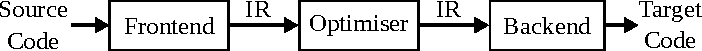
\includegraphics[scale=0.9]{src/background/figs/3-phase-compiler.pdf}
  \caption{Overview of the three-phase compiler infrastructure.}
  \label{fig:3-phase-compiler}
\end{figure}

%The front end parses source code, checking it for errors, and builds a language-specific Abstract Syntax Tree (AST) to represent the input code. The AST is optionally converted to a new representation for optimization, and the optimizer and back end are run on the code.
%The optimizer is responsible for doing a broad variety of transformations to try to improve the code's running time, such as eliminating redundant computations, and is usually more or less independent of language and target.


\begin{figure}[h]
  \centering
  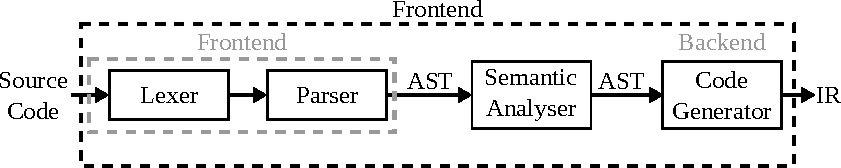
\includegraphics[scale=0.9]{src/background/figs/compiler-frontend.pdf}
  \caption{Overview of the three-phase compiler infrastructure.}
  \label{fig:compiler-frontend}
\end{figure}

\begin{figure}[h]
  \centering
  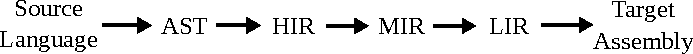
\includegraphics[scale=0.9]{src/background/figs/ir-lowering-sequence.pdf}
  \caption{Overview of the three-phase compiler infrastructure.}
  \label{fig:ir-lowering-sequence}
\end{figure}

\subsection{Link-Time Optimisations}
%% benefits of LTO
%% challenges with LTO
%% mention partial LTO, such as ThinLTO

\begin{figure}[h]
  \centering
  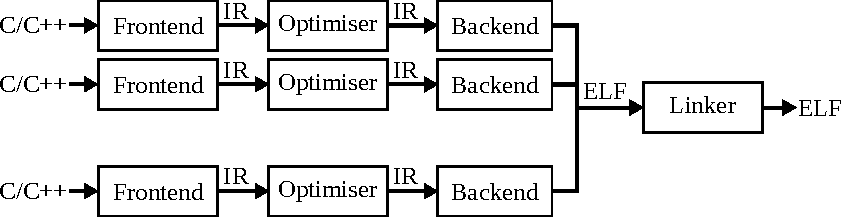
\includegraphics[scale=0.85]{src/background/figs/full-pipeline.pdf}
  \caption{Overview of the three-phase compiler infrastructure.}
  \label{fig:ir-lowering-sequence}
\end{figure}

\begin{figure}[h]
  \centering
  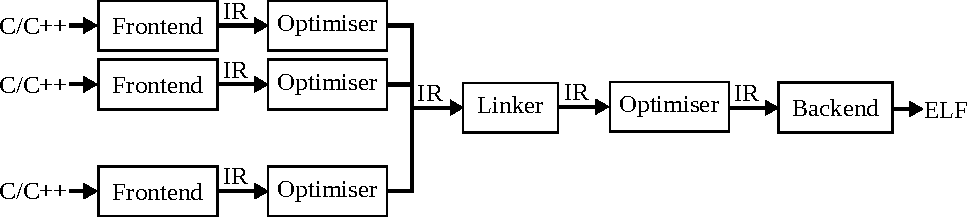
\includegraphics[scale=0.85]{src/background/figs/full-pipeline-LTO.pdf}
  \caption{Overview of the three-phase compiler infrastructure.}
  \label{fig:ir-lowering-sequence}
\end{figure}


\section{Optimisation Scope}
%% describe local optimisations (block level), global (intra-procedural), and inter-procedural (across functions)

\subsection{Interprocedural Optimisations}
%% benefits of IPO
%% challenges involved in IPO



\section{Sequence Alignment}

The comparison of two or more sequences, measuring the extent to which they differ, is important in many scientific areas, most notably in molecular biology~\cite{needleman70,smith81,carrillo88,wang94} where it has been critical
in the understanding of functional, structural, or evolutionary relationships between the sequences~\cite{kruskal83,mount05book}.

A particularly important comparison technique is sequence alignment, which identifies a series of patterns that appear in the same order in the sequences.
Essentially, sequence alignment algorithms insert blank characters in both input sequences so that the final sequences end up having the same size, where equivalent segments are aligned with their matching segments from the other sequence and non-equivalent segments are either paired with the blank or a mismatching character.

Figure~\ref{fig:seq-align-example} shows an example of a pair-wise sequence alignment.
This example, adapted from Lee~et~al.~\cite{lee02}, shows two protein sequences where amino acids are represented by their one-letter symbology~\cite{aasland68}.

\begin{figure}[h]
  \centering
  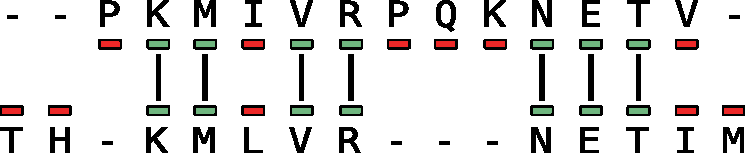
\includegraphics[scale=0.55]{src/background/figs/seq-align-example}
  \caption{Example of an optimum alignment between two sequences.
  Matching segments are shown in green, vertically centred, and the non-matching segments are shown in red at the sides.}
  \label{fig:seq-align-example}
\end{figure}

Formally, sequence alignment can be defined as follows:
For a given alphabet $\alpha$, a sequence $S$ of $k$ characters is an element of
$\alpha^k$, i.e., $S = (a_1, \ldots a_k)$.
Let $S_1, \ldots, S_m$ be a set of sequences, possibly of different lengths but
all derived from the same alphabet $\alpha$, where
$S_i = (a_1^{(i)}, \ldots, a_{k_i}^{(i)})$, for all $i\in\{1,\ldots,m\}$.
Consider an extended alphabet that includes the \textit{blank} character ``$-$'',
i.e., $\beta = \alpha \cup \{-\}$.
An alignment of the $m$ sequences, $S_1, \ldots, S_m$, is another set of sequences,
$\bar{S}_1, \ldots, \bar{S}_m$, such that each sequence $\bar{S}_i$ is obtained
from $S_i$ by inserting blanks in positions where some of the other sequences
have non-blank and possibly equivalent characters, for a given equivalence relation.
All sequences $\bar{S}_i$ in the alignment set have the same length $l$, where
$\max\{k_1,\ldots,k_m\} \leq l \leq k_1 + \cdots + k_m$.
Moreover, $\forall i\in\{1,\ldots, m\}$, $\bar{S}_i = (b_1^{(i)},\ldots,b_l^{(i)})$,
there are increasing functions $v_i: \{1,\ldots,k_i\} \to \{1,\ldots,l\}$, such that:
\begin{itemize}
\item $b_{v_i(j)}^{(i)} = a_j^{(i)}$, for every $j \in \{1,\ldots,k_i\}$;
\item any position not covered by the function $v_i$ contain a black character, i.e., for every $j \in \{1,\ldots,l\}\setminus \textrm{Im} \, v_i$, $b_j$ is the blank character ``$-$''.
\end{itemize}
Finally, for all $j\in\{1,\ldots,l\}$, there is at least one value of $i$ for which $b_j^{(i)}$ is not a blank character.
Note that two aligned sequences may contain both non-blank and non-equivalent characters at any given position, in which case there is a mismatch.

The sequence alignment problem is concerned with identifying an alignment that maximises the score for a given scoring scheme.
The scoring scheme first defines a weight for the alignment of pairs of characters which will then be used to compose a score for the whole sequence alignment.
These weights are used to penalise mismatches and gaps while favouring matching pairs.

The alignment score between two characters is defined by a function on pairs of characters, $\delta \in \beta\times\beta \to \mathbb{R}$, for a given extended alphabet $\beta$.
The simplest function that is commonly used is the constant function~\cite{haque09}.
Let $a,b\in\beta$ and $a \neq b$.
This constant function is defined by a triple $(w_1,w_2,w_3)\in\mathbb{R}^+\times\mathbb{R}^-\times\mathbb{R}^-$, such that:
\begin{itemize}
\item For two matching caracters, $\delta(a,a) = w_1, w_1\in\mathbb{R}^+$.
\item For a mismatch betweem non-blank characters, $\delta(a,b) = w_2, w_2\in\mathbb{R}^-$.
\item The gap penalty, for when we have a blank character, $\delta(a,-) = \delta(-,a) = w_3, w_3\in\mathbb{R}^-$.
\end{itemize}
This is a simple scoring scheme that rewards matches and penalises mismatches and gaps.

There is a vast literature on algorithms for performing sequence alignment, especially in the context of molecular biology.
These algorithms are classified as either global or local.
A global sequence alignment algorithm attempts to align the entire sequence, using as many characters as possible, up to both ends of each sequence.
Global alignment algorithms are useful for sequences that are highly similar and have approximately the same length~\cite{mount05book}.
Alternatively, a local sequence alignment algorithm generates subalignments in stretches of sequence with the highest density of matches.
Local alignments are more suitable for aligning sequences with very few similarities or vastly different lengths~\cite{mount05book}.

In this work, we will focus on pair-wise global alignment algorithms.
The following sections describe the main optimal algorithms based on dynamic programming.
These algorithms will offer different optimality, performance, and memory usage trade-offs~\cite{needleman70,smith81,carrillo88,hickey11}.
%Different alignments would produce different but valid merged functions.

\subsection{Needleman-Wunsch Algorithm}

The Needleman-Wunsch algorithm~\cite{needleman70} is one of the most well known algorithm for pair-wise global alignment.
This algorithm gives an alignment that is guaranteed to be optimal for a given scoring scheme~\cite{higgins89}.

The Needleman-Wunsch algorithm is based on dynamic programming and consists of two main steps.
First, it builds a \textit{similarity matrix}, based on a scoring scheme, which assigns weights for matches, mismatches, and \textit{gaps} (blank characters).
Afterwards, a backward traversal is performed on the similarity matrix, in order to reconstruct the final alignment by maximizing the total score.

\begin{figure}[h]
  \centering
  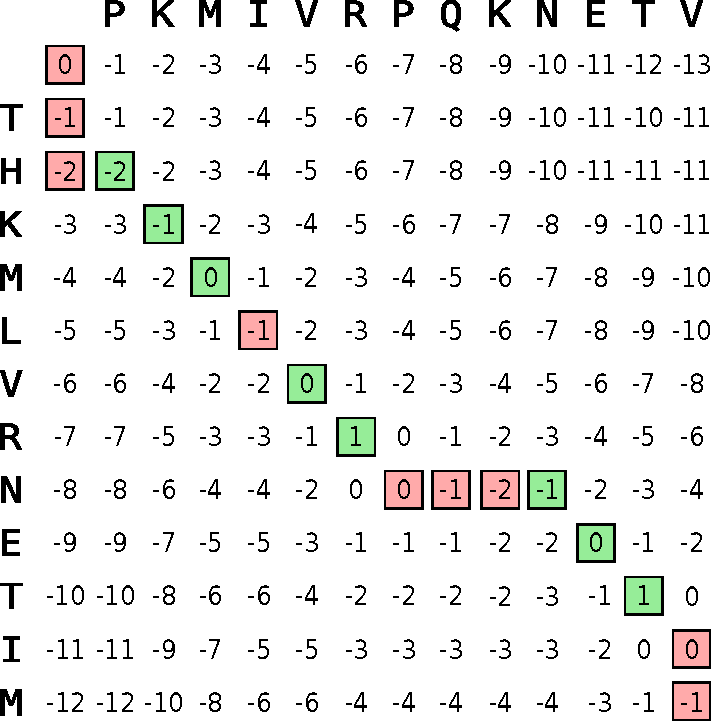
\includegraphics[scale=0.6]{src/background/figs/seq-align-example-nw}
  \caption{Example of the \textit{similarity matrix} computed for two input sequences.
           The highlighted cells represent the resulting alignment computed by the Needleman-Wunsch algorithm.}
  \label{fig:seq-align-example-nw}
\end{figure}

Figure~\ref{fig:seq-align-example-nw} shows the similarity matrix corresponding to the example from Figure~\ref{fig:seq-align-example}.
The similarity matrix is constructed by comparing all possible pairs of characters from the input sequences.
Let $S_1$ and $S_2$ be our input sequences of sizes $k_1$ and $k_2$, respectively, where $S_1 = (a_1,\ldots,a_{k_1})$ and $S_2 = (b_1,\ldots,b_{k_2})$.
The similarity matrix $M$ computed for these two input sequences will have size $(k_1 + 1) \times (k_2+1)$.
Let $M_{i,j}$ denote all entries in the similarity matrix, with $1 \leq i \leq (k_1 + 1)$ and $1 \leq j \leq (k_2 + 1)$.
The first entry in the matrix is $M_{1,1} = 0$, and
\begin{equation*}
%\begin{align*}
M_{i,j} = \max \begin{cases}
  M_{i-1,j} + \delta(a_{i-1},-)         &  \quad  \text{if } i>1 \text{ and } j\geq1 \\
  M_{i,j-1} + \delta(-,b_{j-1})         &  \quad  \text{if } i\geq1 \text{ and } j>1 \\
  M_{i-1,j-1} + \delta(a_{i-1},b_{j-1}) &  \quad  \text{if } i>1 \text{ and } j>1
\end{cases}
%\end{align*}
\end{equation*}
In other words, the score for each cell in the similarity matrix is the maximum among the rules shown in Figure~\ref{fig:seq-align-rules}.

\begin{figure}[h]
  \centering
  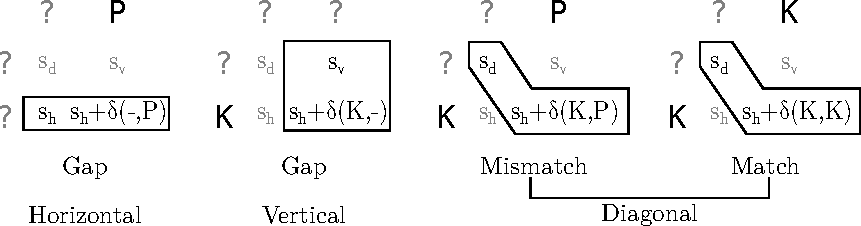
\includegraphics[scale=0.8]{src/background/figs/seq-align-rules}
  \caption{Set of rules used to compute the scores of the similarity matrix.
           The two first rules represent the penalty of inserting a horizontal or vertical gap.
           The diagonal rule depends whether we have a matching or mismatching pair of input characters.}
  \label{fig:seq-align-rules}
\end{figure}


Figure~\ref{fig:seq-align-example-nw} also highlights the traversal. 
Note that sometimes, while traversing the score matrix, there are multiple adjacent neighbours with the same score.
Since there may exist multiple traversals with the same score, two sequences can have multiple optimum alignments.

Needleman-Wunsh algorithm is quadratic in the size of the sequences being aligned, both in time and space.

%\subsection{Hirschberg Algorithm}

\chapter{Related Work}

\section{Code-Size Optimisations}

Although initially motivated by performance, many of the classical optimisations achieve better performance by reducing code size.
A small code, besides having fewer instructions to execute, can also have a positive impact on the cache utilisation.
Classical optimisations that are effective in reducing code size include the elimination of redundant, unreachable, and dead code, as well as certain kinds of strength reduction~\cite{cocke70,briggs97,debray00}.
In this section, we will describe some of these classical size-reducing optimisations.

\subsection{Constant Folding}

Constant folding is an optimisation that operates on the instruction level, identifying instructions whose operands are constant values, performing the evaluation of the instruction at compile time, and replacing it by the resulting value.
The effectiveness of constant folding can be augmented by combining it with constant propagation.
Constant folding reduces code size by eliminating instructions that can be computed at compile time.
Moreover, constant folding also works as an enabler to other optimisations, such as unreachable-code elimination (Section~\ref{sec:relatedwork:unreachable}).
 
\subsection{Unreachable-Code Elimination} \label{sec:relatedwork:unreachable}

Some functions may contain code that is unreachable. A code is unreachable if there is no valid control-flow path from the function's entry point that leads to it.
Since unreachable code is guaranteed to never be executed, compilers should remove it to avoid code bloat.

Often, unreachable code is uncovered by other optimisations.
For example, after constant propagation and constant folding, a conditional branch could have its condition evaluating to a constant, eliminating a path to one of its successor basic block.
If no other path leads to that basic block, it becomes unreachable.

The algorithm to eliminate unreachable code works in a mark-sweep manner, performing two passes over the basic blocks of the CFG.
The reachability analysis optimistically assumes that all basic blocks are dead until proven otherwise.
First, it marks all blocks as unreachable.
Next, starting from the entry point, it marks each block that it can reach as reachable.
If all branches and jumps are unambiguous, then all unmarked blocks can be deleted.
With ambiguous branches or jumps, the compiler must preserve any block that the branch or jump can reach.
This analysis is simple and inexpensive.

\subsection{Dead-Code Elimination}

A value definition is dead if it is not used on any path from the point in which it is defined to the exit point of the function.
In a similar way, an instruction is dead if it computes only values that are not used on any execution path leading from the instruction.
Any dead definition or instruction can be simply removed without altering the program's semantics, therefore reducing code size~\cite{muchnick98}.

The algorithm to eliminate dead code has some similarities with that for unreachable-code elimination described in Section~\ref{sec:relatedwork:unreachable}.
This algorithm also works in a mark-sweep manner~\cite{cooper07}.
First, the algorithm marks \textit{critical} instructions as \textit{alive}.
An instruction is \textit{critical} if it has an observable effect, for example, if it is a return instruction, a branch instruction, a function call, a memory operation, any instruction with side effect, etc.
Then, the algorithm follows the \textit{use-def chain} of every alive instruction, marking the operand instructions as alive.
This process continues until no more instructions can be marked as alive.
Finally, the sweep phase removes all instructions that have not been marked as alive, reducing code size.

\section{Merging Identical Functions}

In this section, we will discuss existing optimisations for merging identical functions.
Figure~\ref{fig:example-identical} illustrates how identical functions can appear in real programs.
The first pair of functions, shown in Figure~\ref{fig:example-identical-1-sphinx3}, were extracted from the \texttt{482.sphinx3} benchmark.
The only difference between these two functions is in their parameter type.
However, all pointer types can be considered equivalent since they can be bitcasted in a losslessly way.
These functions are usually produced by copy-and-paste programming, where a given code pattern is copied and then repurposed~\cite{kim04,jablonski10,ahmed15}.
The second pair of functions, shown in Figure~\ref{fig:example-identical-2-gcc}, were extracted from the \texttt{403.gcc} benchmark and they are fully identical.
These functions are part of GCC's backend, where it is common to have code that is automatically generated from a machine description~\cite{muchnick98,kolek13,ghica15}.

\begin{figure}[h]
\centering
\begin{subfigure}{\textwidth}
\centering
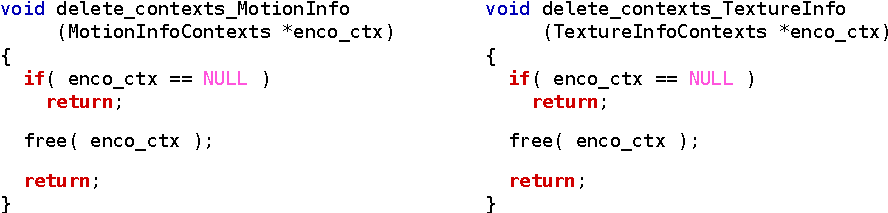
\includegraphics[scale=0.9]{src/relatedwork/figs/example-identical-1-sphinx3}
\caption{Two semantically identical functions extracted from the \texttt{482.sphinx3} benchmark.}
\label{fig:example-identical-1-sphinx3}
\end{subfigure}
\begin{subfigure}{\textwidth}
\centering
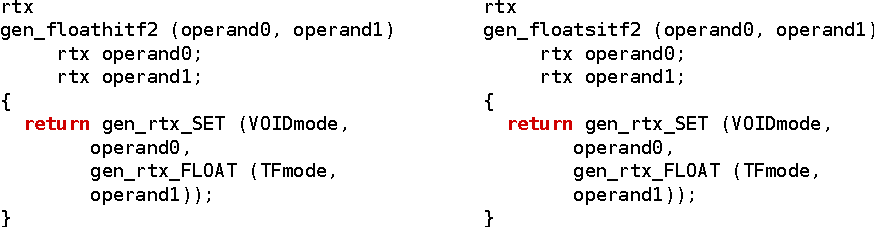
\includegraphics[scale=0.9]{src/relatedwork/figs/example-identical-2-gcc}
\caption{Two semantically identical functions extracted from the \texttt{403.gcc} benchmark.}
\label{fig:example-identical-2-gcc}
\end{subfigure}
\caption{Example of identical functions.}
\label{fig:example-identical}
\end{figure}

\begin{figure}[h]
\centering
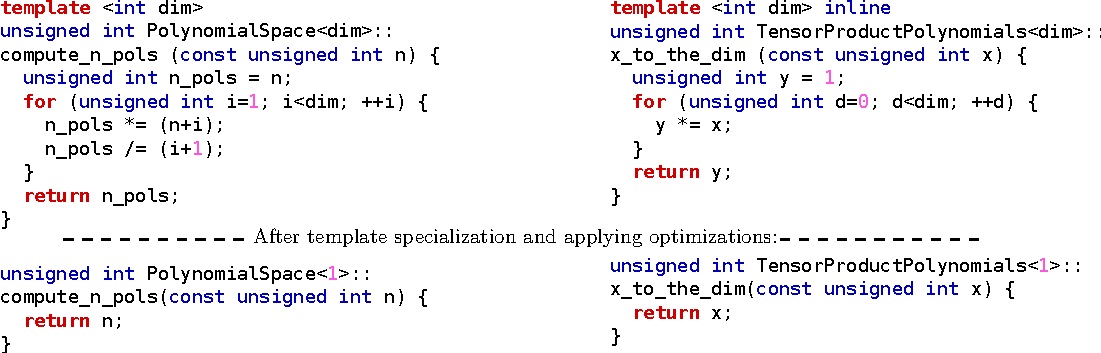
\includegraphics[scale=0.9]{src/relatedwork/figs/identical-example}
\caption{Two function extracted from the \texttt{447.dealII} benchmark that are not identical at the source level, but after applying template specialisation and optimisations they become identical at the IR level.}
\label{fig:identical-example}
\end{figure}

Note, however, that functions can be identical at the IR or machine level without necessarily being identical at the source level.
Figure~\ref{fig:identical-example} shows two real functions extract from the
447.dealII program in the SPEC CPU2006~\cite{spec} benchmark suite.
Although these two functions are not identical at the source level, they become
identical after a template specialisation and some optimisations are applied, in
particular, constant propagation, constant folding, and dead-code elimination. 
Specialising \verb|dim| to $1$ enables to completely remove the loop in the
function \verb|PolynomialSpace|.
Similarly, specializing \verb|dim| to $1$ results in only the first iteration
of the loop in the function \verb|TensorProductPolynomials| being executed.
The compiler is able to statically analyze and simplify the loops in both
functions, resulting in the identical functions shown at the bottom of
Figure~\ref{fig:identical-example}.

Identical code is particularly common in C++ programs
with heavy use of \textit{parametric polymorphism}, via template or \textit{auto} type deduction.



\section{Merging Identical Object Code}

The simplest way of merging identical functions is by looking at their object code, during link time.
\textit{Identical code folding}~(ICF) is an optimisation that identifies and merges two or more read-only sections, typically functions, that have identical contents.
This optimisation is commonly found in major linkers, such as \textit{gold}~\cite{tallam10,kwan12}, LLVM's \textit{lld}, and the MSVC linker~\cite{msvc-icf}.

Figure~\ref{fig:icf-example} shows an example, adapted from Tallam~\etal~\cite{tallam10},
of how generic programming in C++ can lead to identical functions in the object file.
The C++ code in in Figure~\ref{fig:icf-example-code} presents
a simple \textit{template class} and its member function being
instantiated multiple times with different pointer types.
Figure~\ref{fig:icf-example-object} shows the object code 
targeting the Intel x86 architecture.
For each instantiation of \textit{Foo}, a replica of its member
function \textit{getElement} is created.
Because the size of the different pointer types is the same,
all replicas of \textit{getElement} are identical
in the object file, which can be easily confirmed by
comparing their binary representation. as shown in
Figure~\ref{fig:icf-example-object}.

\begin{figure}[h]
% \begin{tabular}{cc}
% \begin{subfigure}{.5\textwidth}
% \begin{minted}[
% frame=lines,
% framesep=2mm,
% baselinestretch=1,
% %bgcolor=LightGray,
% fontsize=\footnotesize,
% %linenos
% ]{c++}
% template<typename T>
% class Foo {
%   ...
%   T element;
% public:
%   ...
%   T getElement() {
%     return element;
%   }
% };

% int main() {
%   Foo<int *> p;
%   Foo<float *> q;
%   Foo<void *> r;
%   ...
%   auto *pptr = p.getElement();
%   auto *qptr = q.getElement();
%   auto *rptr = r.getElement();
%   ...
% }
% \end{minted}
% \caption{A \textit{template class} with several instantiations.}
% \label{fig:icf-example-code}
% \end{subfigure} &
% \begin{subfigure}{.5\textwidth}
% \vspace{10ex}
% \begin{minted}[
% escapeinside=||,
% %fontfamily=tt,
% frame=lines,
% framesep=2mm,
% baselinestretch=1,
% %bgcolor=LightGray,
% fontsize=\scriptsize,
% %linenos
% ]{nasm}
% ; Disassembly of Foo<int *>::getElement()
% section .text._ZN3FooIPiE10getElementEv:
% _ZN3FooIPiE10getElementEv:   ; Hex Code
%   mov  rax,QWORD PTR [rdi]  ; 48 8b 07
%   ret                        ; c3

% ; Disassembly of Foo<float *>::getElement()
% section .text._ZN3FooIPfE10getElementEv:
% _ZN3FooIPfE10getElementEv:   ; Hex Code
%   mov  rax,QWORD PTR [rdi]  ; 48 8b 07
%   ret                        ; c3

% ; Disassembly of Foo<void *>::getElement()
% section .text._ZN3FooIPvE10getElementEv:
% _ZN3FooIPvE10getElementEv:   ; Hex Code
%   mov  rax,QWORD PTR [rdi]  ; 48 8b 07
%   ret                        ; c3
% \end{minted}
% \vspace{7ex}
% \caption{Disassembled object file.}
% \label{fig:icf-example-object}
% \end{subfigure}
% \end{tabular}
\caption{Example showing how a member function of a \textit{template class}
  can produce code replication susceptible to \textit{identical code folding}.
  For each instantiation of \textit{Foo}, a replica of the function
  \textit{getElement} is created for the template instance.
  When instantiated with pointer types, the object code of these functions will be identical.}
\label{fig:icf-example}
\end{figure}

Most object file formats, such as the \textit{Executable and Linkable Format} (ELF)~\cite{tallam10,kwan12}, are structured as separate sections of content, each section containing a certain type of content.
The main types are code segment, different types of data segment, and relocation information.
Relocation information describes how to modify other sections, connecting symbolic references to their definition.
In other words, it assigns actual addresses for position-dependent code and data.
For example, when a program calls a function, the associated call instruction must transfer control to the proper destination address at execution.

It is common practice for linkers to place functions in separate sections, as exemplified in Figure~\ref{fig:icf-example-object}.
Therefore, merging identical functions can be generalised to the problem of merging identical sections.
Two sections are considered identical if they have the identical section flags, data, code, and relocations.
Two relocations are considered the identical if they have the same relocation types, values, and if they point to the same or identical sections.

Since this equality has a cyclic definition, ICF is defined as a fixed-point computation, i.e., it is applied repeatedly until a convergence is obtained.
There are two approaches with distinct trade-offs.
$(i)$ The pessimistic apprach starts with all sections marked as being different and then repeatedly compare them trying to prove their equality, grouping those found to be identical, including their relocations.
This approach is implemented in the widely used \textit{gold} linker.
$(ii)$ The optimistic apprach starts with all functions marked as potentially identical and then repeatedly compare trying to disprove their equality, partitioning those found to be different.
This approach is implemented in LLVM's linker, \textit{lld}.

% \subsection{The Pessimistic Algorithm}

% The pessimistic algorithm is implemented in the gold linker.

% We can start with marking all functions as different and repeatedly do
% the checksumming.  This has the advantage that we do not need to wait
% for convergence. We can stop at any point and correctness will be
% guaranteed although not all cases would have been found.  However, this
% has a problem that some cases can never be found even if it is run until
% convergence.  Here is an example with mutually recursive functions :

% int funcA (int a)            int funcB (int a)
% {                            {
%   if (a == 1)                  if (a == 1)
%     return 1;                    return 1;
%    return 1 + funcB(a - 1);     return 1 + funcA(a - 1);
% }                            }

% In this example funcA and funcB are identical and one of them could be
% folded into the other.  However, if we start with assuming that funcA
% and funcB are not identical, the algorithm, even after it is run to
% convergence, cannot detect that they are identical.


% \subsection{The Optimistic Algorithm}

% The optimistic algorithm is implemented in LLVM linker, lld.

\begin{figure}[h]
% \begin{tabular}{cc}
% \begin{subfigure}{.5\textwidth}
% \begin{minted}[
% frame=lines,
% framesep=2mm,
% baselinestretch=1,
% %bgcolor=LightGray,
% fontsize=\footnotesize,
% %linenos
% ]{c++}
% int zip() {
%   return 0;
% }
% int zap() {
%   return 0;
% }
% int foo() {
%   return zip ();
% }
% int bar() {
%   return zap ();
% }
% \end{minted}
% \caption{A \textit{template class} with several instantiations.}
% \label{fig:icf-example-code}
% \end{subfigure} &
% \begin{subfigure}{.5\textwidth}
% \begin{minted}[
% escapeinside=||,
% frame=lines,
% framesep=2mm,
% baselinestretch=1,
% %bgcolor=LightGray,
% fontsize=\scriptsize,
% %linenos
% ]{gas}

% section .text._Z3zipv:
% _Z3zipv:                 ; Hex Code
%  xor eax, eax            ; 31 c0
%  ret                     ; c3    

% section .text._Z3zapv:
% _Z3zapv:
%  xor eax, eax            ; 31 c0
%  ret                     ; c3

% section .text._Z3foov:
% _Z3foov:
%  push rax                ; 50
%  call   6 |<\_Z3foov+0x6>|  ; e8 00 00 00 00
%  pop rcx                 ; 59
%  ret                     ; c3
% section .rela.text._Z3foov ; Relocation
% ; Type         Addend  Name
%  X86_64_PC32    -4      _Z3zipv

% section .text._Z3barv:
% _Z3barv:
%  push rax                ; 50
%  call   6 |<\_Z3barv+0x6>|  ; e8 00 00 00 00
%  pop rcx                 ; 59
%  ret                     ; c3
% section .rela.text._Z3barv ; Relocation
% ; Type         Addend  Name
%  X86_64_PC32    -4      _Z3zapv

% \end{minted}
% \caption{Disassembled object file.}
% \label{fig:icf-example-object}
% \end{subfigure}
% \end{tabular}
\begin{subfigure}{\textwidth}
\centering
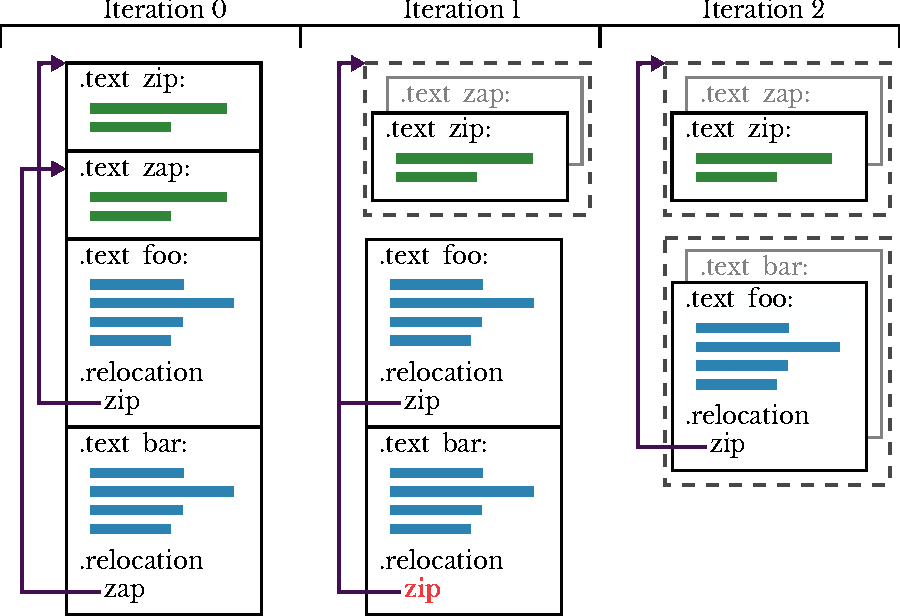
\includegraphics[width=0.9\textwidth]{src/relatedwork/figs/icf-example}
\caption{.}
\label{fig:identical-example}
\end{subfigure}

\caption{Example showing how a member function of a \textit{template class}
  can produce code replication susceptible to \textit{identical code folding}.
  For each instantiation of \textit{Foo}, a replica of the function
  \textit{getElement} is created for the template instance.
  When instantiated with pointer types, the object code of these functions will be identical.}
\label{fig:icf-example}
\end{figure}


\subsection{Identical Function Merging}

A similar optimisation for merging identical functions, but instead at the
intermediate representation (IR) level, is also offered by both GCC and
LLVM~\cite{llvm-fm,livska14}.
%The function merging optimisation currently offered by LLVM is only able to
%merge identical functions.
This optimisation is only flexible enough to accommodate simple type mismatches
provided they can be bitcasted in a losslessly way.

%%%%%%%%%%%%%%%%%%%%%%%%%%%%%%%%%%%%%%%%%%%%%%%%%%%%%%%%%%%%%%%%%%%%%%%%%%%%%%%%

A very strict function comparator is used to identify if two functions are 
semantically equivalent.
First it compares the signature and other general attributes of the two functions.
The functions must have identical signature, i.e., the same return type, the same
number of arguments, and exactly the same list of argument types.
Then this function comparator performs a simultaneous walk, in depth
first order, in the functions' control-flow graphs.
This walk starts at the entry block for both functions, then takes each block
from each terminator in order.
As an artifact, this also means that unreachable blocks are ignored.
Finally, it iterates through each instruction in each basic block.
Two blocks are equivalent if they have equivalent instructions in exactly the
same order, without excess.
The comparator always fails conservatively, erring on the side of claiming that
two functions are different.

When a pair of equivalent functions is identified, we can create either
an alias or a \textit{thunk}.
Aliasing etails eliminating one of the functions and replacing all its callsites
to the other function.
Thunks must be created when neither of the equivalent functions can be eliminated
by aliasing.
In such case, a thunk is created for either one of the functions, replacing its
body by a call to the other function, which allows all callsites and name
references to both functions to be preserved.
%In such case, the body of one of the functions is replaced by a call to the
%other function, and all callsites to both functions are preserved.
Aliasing is prefered since it is cheaper and adds no runtime overhead.
The appropriate merging is applied according to following rules:
\begin{itemize}
\item If the address of at least one function is not taken, alias can be used.
\item But if the function is part of COMDAT section that can be replaced, we
must use thunk.
\item If we create a thunk and none of functions is writeable, we can redirect calls
instead.
\end{itemize}
%%%%%%%%%%%%%%%%%%%%%%%%%%%%%%%%%%%%%%%%%%%%%%%%%%%%%%%%%%%%%%%%%%%%%%%%%%%%%%%%
%Similarly to the technique proposed by Edler von Koch~et~al.~\cite{edler14},
%LLVM's optimisation also exploits structural similarity among functions.
%However, the current implementation does not allow instructions to differ in
%their opcodes or in the number and type of their input operands.
Although very restrictive, this optimisation guarantees that any pair of
mergeable functions will result in code size reduction with no performance
overhead.

%Its simplicity also benefits compilation time, as the actual merge operation
%is trivial.
Its simplicity also allows for an efficient exploration approach based on computing
a hash of the functions and then using a binary tree to identify equivalent
functions.
%%%%%%%%%%%%%%%%%%%%%%%%%%%%%%%%%%%%%%%%%%%%%%%%%%%%%%%%%%%%%%%%%%%%%%%%%%%%%%%%
%We define a congruent group as a set of functions that are candidates for
%function equality.
%To create congruent groups, we build a compound hash value for each previously
%parsed function.
%%%As an optimisation, a hash of the function structure is calculated first, and
%%%two functions are only compared if they have the same hash.
Since hashing is cheap to compute, it allows us to efficiently
%Hashing is used to
group possibly equivalent functions and filter out functions
that are obviously unique.
%This hash is cheap to compute,
This hash must have the property that if function $F = G$
according to the comparison function, then $hash(F) = hash(G)$.
Therefore, as an optimisation, two functions are only compared if they have the
same hash.
This consistency property is critical to ensuring all possible merging
opportunities are exploited.
Collisions in the hash affect the speed of the pass but not the correctness
or determinism of the resulting transformation.

A function hash is calculated by considering only the number of arguments and
whether a function is varargs, the order of basic blocks (given by the
successors of each basic block in depth first order), and the order of
opcodes of each instruction within each of these basic blocks.
This mirrors the strategy of compare() uses to compare functions by walking the BBs in depth
first order and comparing each instruction in sequence. Because this hash
does not look at the operands, it is insensitive to things such as the
target of calls and the constants used in the function, which makes it useful
when possibly merging functions which are the same modulo constants and call
targets.


All functions can be sorted based on their hash value, which ends up grouping
possibly equivalent functions together.
If the hash value of a given function matches any of its adjacent values in
the sorted list, this function must be considered for merging.
%After that, the pass sorts each function to a congruent class according to
%its hash value.
%All functions in the module, ordered by hash.
Functions with a unique hash value can be easily ignored since no other function
will be found equivalent.
%Functions with a unique hash value are also easily eliminated.
%Otherwise it is dropped and never considered again.


The functions that remain are inserted into a binary tree, where functions are
the node values themselves.
An order relation is defined over the set of functions.
We need total-ordering, so we need to maintain four properties on the functions set:
\begin{itemize}
\item $a <= a$ (reflexivity);
\item if $a <= b$ and $b <= a$ then $a = b$ (antisymmetry);
\item if $a <= b$ and $b <= c$ then $a <= c$ (transitivity);
\item for all $a$ and $b$, $a <= b$ or $b <= a$ (totality).
\end{itemize}
This total-ordering was made through special function comparison procedure that
returns:
\begin{itemize}
\item 0 when functions are semantically equal,
\item -1 when Left function is less than right function, and
\item 1 for opposite case.
\end{itemize}

Functions are kept on binary tree. For each new function F we perform
lookup in binary tree.

%After the previous step is finished, all candidates in a group must be proved to
%be really semantically equivalent.

%Therefore, by construction, functions are hashed and grouped in O(n log n) time
%complexity.






\section{Merging Beyond Identical Functions}

In the previous sections, we have seen compiler optimisations that merge identical functions.
However, nearly identical functions, with only minor differences, are also commonly found.
Figure~\ref{fig:example-similar} shows two examples of nearly identical functions found in real programs.
The highlighted differences prevent these functions from being merged by the identical function merging techniques.
%These functions are usually produced by copy-and-paste programming,
%where a given code pattern is copied and then repurposed~\cite{kim04,jablonski10,ahmed15}.
The first pair of functions, shown in Figure~\ref{fig:example-similar-1-hmmer}, illustrates code that is usually produced by copy-and-paste programming,
where a given code pattern is copied and then repurposed~\cite{kim04,jablonski10,ahmed15}.
The second pair of functions, shown in Figure~\ref{fig:example-similar-3-gcc}, are produced by generative programming~\cite{czarnecki99,draheim04}, where their code was
automatically generated using a description language~\cite{ghica15}.

\begin{figure}[h]
\centering
\begin{subfigure}{\textwidth}
\centering
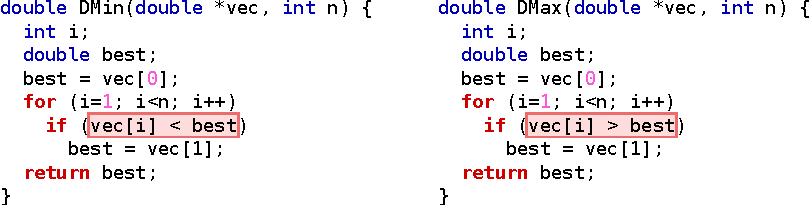
\includegraphics[width=0.9\textwidth]{src/relatedwork/figs/example-similar-1-hmmer}
\caption{Two similar functions extracted from the \texttt{456.hmmer} benchmark.}
\label{fig:example-similar-1-hmmer}
\end{subfigure}
%\begin{subfigure}{\textwidth}
%\centering
%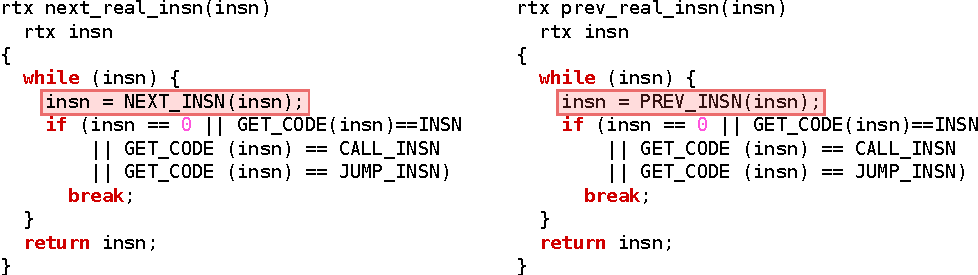
\includegraphics[width=0.9\textwidth]{src/relatedwork/figs/example-similar-2-gcc}
%\caption{Two similar functions extracted from the \texttt{403.gcc} benchmark.}
%\label{fig:example-similar-2-gcc}
%\end{subfigure}
\begin{subfigure}{\textwidth}
\centering
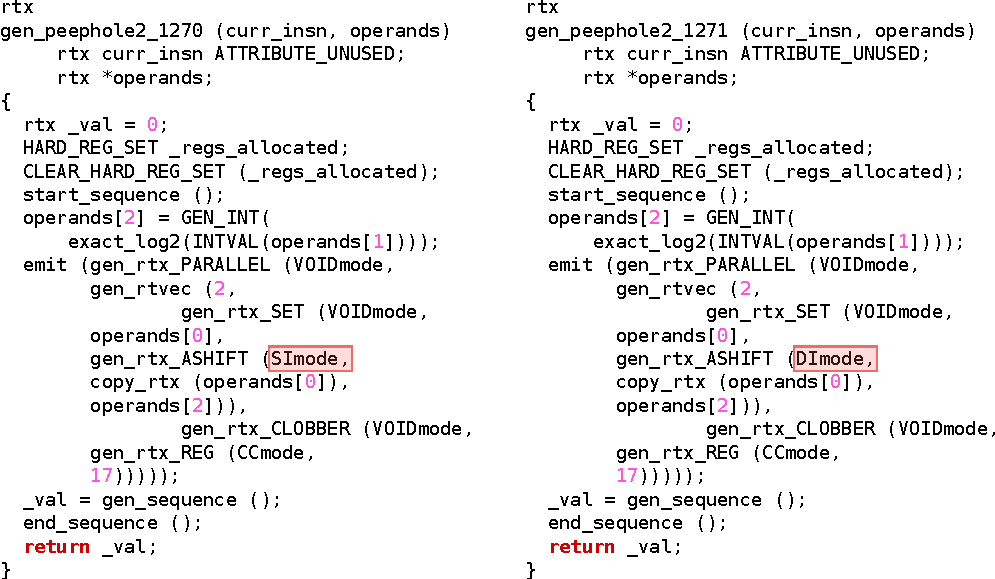
\includegraphics[width=\textwidth]{src/relatedwork/figs/example-similar-3-gcc}
\caption{Two similar functions extracted from the \texttt{403.gcc} benchmark.}
\label{fig:example-similar-3-gcc}
\end{subfigure}
\caption{Example of two pairs of highly similar functions. Because they are not identical, they cannot be merged by the function merging technique currently found in major compilers.}
\label{fig:example-similar}
\end{figure}


% The function merging technique presented in \cite{edler14} restricts merging to nearly identical functions.
% They only allow for pairs of corresponding instructions to differ if they still have equivalent data type.


Edler von Koch~et~al.~\cite{edler14} have proposed a function-merging technique which exploits structural similarity among functions.
Their optimization is able to merge nearly identical functions.
%similar functions that are not necessarily identical.
Two functions are structurally similar if both their function types are equivalent
and their CFGs are isomorphic.
Two function types are equivalent if they agree in the number, order, and types
of their parameters as well as
their return types, linkage type, and other compiler-specific properties.
In addition to the structural similarity of the functions, their technique also
requires that corresponding basic blocks have exactly the same number of instructions
and that corresponding instructions must have equivalent resulting types.
% but may differ in their opcodes or in the number and type of their input operands.
Mergeable functions are only allowed to differ in corresponding instructions,
where they can differ in their opcodes or in the number and type of their input operands.
Corresponding named values must have the same data type.
%The only differences that are actually allowed is that
%corresponding instructions can 
%differ in their opcodes or in the number and type of their input operands.


%If two corresponding instructions have different opcodes, they split the basic
%block and insert a switch branch to select which instruction to execute
%depending on a function identifier.

Because their technique is limited to functions with identical CFGs
and function types, once it merges a pair of functions, a third
\textit{similar} function cannot be merged into the resulting merged function
since they will differ in both CFGs and their lists of parameters.
Due to this limiting factor, the state-of-the-art has to first group
mergeable functions before simultaneously merging all functions within a group.

Their algorithm iterates simultaneously over corresponding basic
blocks in the set functions being merged, as they have isomorphic CFGs.
Figure~\ref{fig:soa-example-1} shows an example of two functions with isomorphic CFGs and their corresponding basic blocks arranged side by side.

\begin{figure}[h]
  \centering
  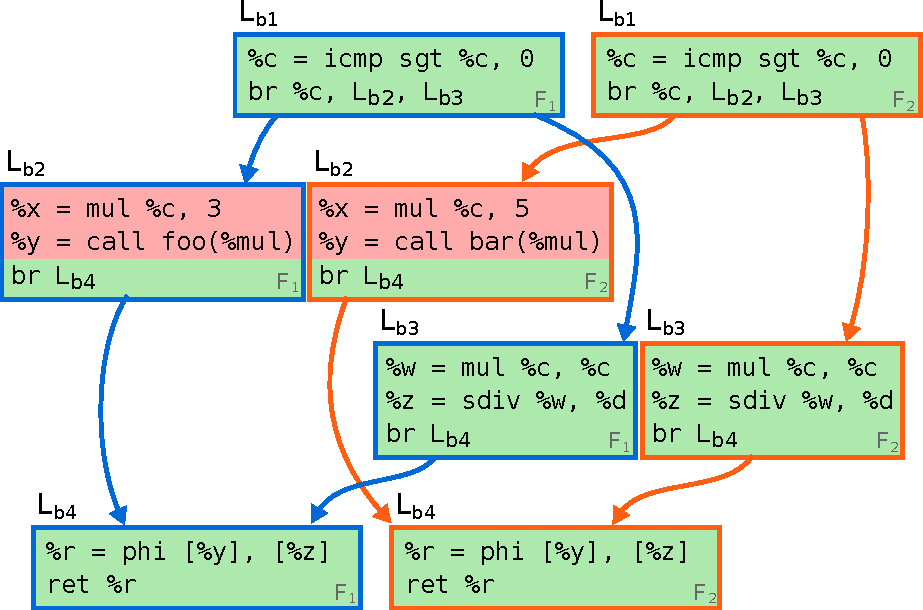
\includegraphics[width=0.8\textwidth]{src/relatedwork/figs/soa-example-1.pdf}
  \caption{An example of two functions with isomorphic CFGs and their corresponding basic blocks arranged side by side. Instructions in paired basic blocks are compared in a pairwise manner.}
  \label{fig:soa-example-1}
\end{figure}

Every pair of basic blocks have their instructions analysed in a pairwise manner.
Two instructions match if they have the same opcode with equivalent data types and operands.
Even if two instructions differ only on their operands, they are classified as mismatching.
For every pair of basic blocks, if their corresponding instructions have any difference, except for the data type of the computed value, the merged basic block is split by inserting a switch branch to select which instruction
to execute depending on a function identifier.
A phi-node is used to unify the mismatching instructions as a single named value.
This unification is only possible because they compute values of the equivalent data types.
Note that no operand selection is performed, every use of the mismatching instructions will refer to their phi-node.
Figure~\ref{fig:soa-example-2} shows an example of a merged basic block containing two mismatching pairs of instructions.
A split is added for every pair of mismatching instructions with the phi-node instruction added to the their immediate point of convergence.

% Because these instructions have equivalent resulting types, their results can be
% merged using a phi-operator, which can then be used transparently as operands
% by other instructions.

\begin{figure}[h]
  \centering
  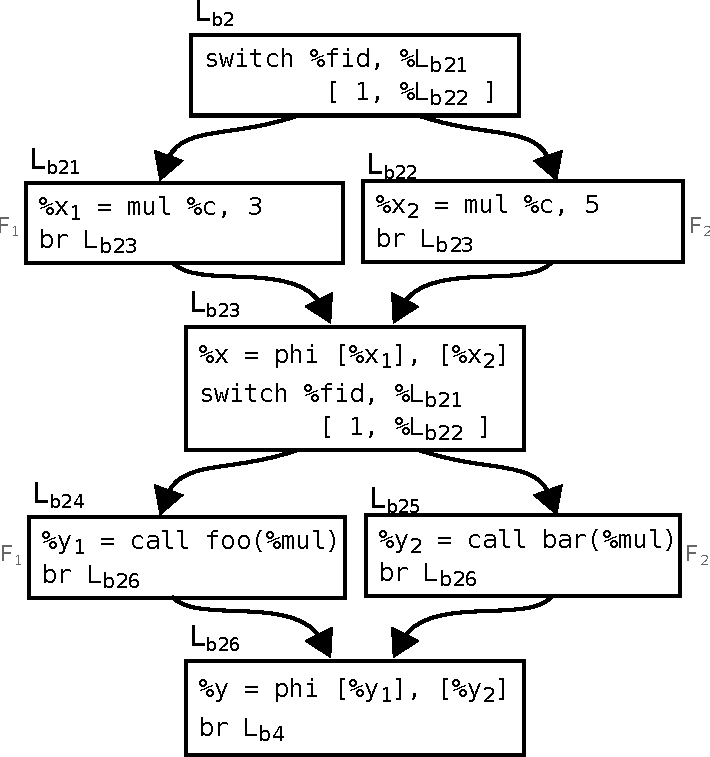
\includegraphics[width=0.6\textwidth]{src/relatedwork/figs/soa-example-2.pdf}
  \caption{An example of a merged basic block containing two mismatching pairs of instructions. A split is added for every pair of mismatching instructions with the phi-node instruction added to the their immediate point of convergence.}
  \label{fig:soa-example-2}
\end{figure}

Overall, except for mismatching pairs of instructions, the two functions must have identical function types, i.e., they must have the same return type and list of arguments, identical CFGs, with corresponding basic blocks having the same number of instructions.
Although this technique improves over LLVM's identical function merging, it is
still unnecessarily limited.
In Section~\ref{sec:motivation}, we showed examples of very similar real functions where the technique proposed by Edler von Koch~et~al.~\cite{edler14} fails to merge.
In Chapter~\ref{chp:cgo19} we introduce a novel technique that addresses such limitations improving on their technique across the board.

%%%%%%%%%%%%%%%%%%%%%%%%%%%%%%%%%%%%%%%%%%%%%%%%%%%%%%%%%%%%%%%%%%%%%%%%



\textbf{TODO: Comparison table: Identical vs VonKoch vs Ours}


\section{Code Factoring}

%Function merging and code factoring are different techniques for solving the
%same fundamental problem of duplicated code.
Code factoring refers to related techniques that address the same fundamental
problem of duplicated code in a different way.
%While the former works by merging similar functions, the latter works by
%factoring out duplicated code~\cite{loki04}.
%Instead of merging similar functions, code factoring works by factoring out
%duplicated code into separate functions~\cite{loki04}.
Code factoring can be applied at different levels of the program~\cite{loki04}.
Local factoring, also known as local code motion, moves identical instructions
from multiple basic blocks to either their common predecessor or successor,
whenever valid~\cite{knoop94,briggs94,loki04}.
Procedural abstraction %(or outlining)
finds identical code
that can be extracted into a separate function, replacing all replicated
occurrences with a function call~\cite{loki04,dreweke07}.

Procedural abstraction differs from function merging as it usually works on
single basic blocks or single-entry single-exit regions.
Moreover, it only works for identical segments of code, and every identical
segment of code is extracted into a separate new function.
Function merging, on the other hand, works on whole functions, which can be
identical or just partially similar, producing a single merged function.

However, all these techniques are orthogonal to the proposed optimization and
could complement each other at different stages of the compilation pipeline.




\section{Code Similarity}

Code similarity has also been used in other compiler optimizations or tools for
software development and maintenance.
In this section, we describe some of these applications.

Coutinho~et~al.~\cite{coutinho11} proposed an optimization that uses instruction
alignment to reduce divergent code for GPU.
They are able to fuse divergent branches that contain single basic blocks,
improving GPU utilization.
%reducing idle cores.

Similarly, analogous algorithms have also been suggested to identify the
differences between two programs, helping developers with source-code
management and maintenance~\cite{yang91,miller85}.
These techniques are applied in tools for source-code management, such as
the \textit{diff} command~\cite{miller85}.

Similar techniques have also been applied to code editors and IDEs~\cite{toomim04,sajnani16}.
For example,
SourcererCC~\cite{sajnani16} detects possible clones, at the source level, by
dividing the programs into a set of code blocks where each code block is itself
represented by a bag-of-tokens, i.e., a set of tokens and their frequencies.
Tokens are keywords, literals, and identifiers, but not operators.
Code blocks are considered clones if their degree of similarity is higher than
a given threshold.
In order to reduce the number of blocks compared, candidate blocks are filtered
based on a few of their tokens where at least one must match.

Our ranking mechanism uses an approach similar to SourcererCC, where we use
opcode frequencies and type frequencies to determine if two functions are
likely to have similar code.
However, we need a precise and effective analysis of code similarity when
performing the actual merge.
To this end, we use a sequence alignment technique.



\section{Tuning Compilers with Deep Learning}

There is been many work using machine learning as a heuristic for tuning runtime systems~\cite{andreasson02,wang09,castro11,rocha17,pereira17} and compilers~\cite{cavazos05,leather09,cummins17,wang18,mendis19}.

Cavazos and O'Boyle~\cite{cavazos05} propose the use of genetic algorithm to tune the heuristics of function inlining.
They use genetic algorithm to optimise the values for different features that control the inlining heuristic.
%Some of these features are the size of the callee and caller functions.
These features are chosen by the compiler writer and they define the maximum size allowed by the inlining transformation for the callee and the caller functions, the maximum size for callee functions that are hot or that should always be inlined, etc.
The optimised features are then used to define the rules of the inlining heuristic, describing which call sites should be allowed for inlining.
The fitness function of the genetic algorithm involves the actual runtime of the compiled program, rendering the feature optimisation process very costly.
However, their approach is able to achieve significant speedups over the baseline.

The quality of these features is critical to the improvements resulting from machine learning solutions.
Leather~et~al.~\cite{leather09} propose the use of genetic programming in order to also automate the selection of these features.
The feature space is described by a grammar and is then searched with genetic programming and predictive modelling, to avoid recompilation of the program for each step in searching the optimization space.
The genetic programming technique is used to generate features that are fed to a decision tree.
This machine learning solution form the decision-making heuristics for the loop-unrolling optimisation.
They show that the automated selection of features outperform hand-coded features, for the same machine learning procedure based on decision trees.

Cummins~et~al.~\cite{cummins17} propose DeepTune, which uses deep neural networks to learn optimization heuristics directly on raw code, unifying the search for features and decision-making heuristics into a single learning model.
Since the program, in its textual form, can be seen as a sequence of tokens of variable length, using a recurrent neural networks becomes a natural choice.
DeepTune has an LSTM-based language model that processes raw code, producing a fixed-size encoding which is then fed to a heuristic model based on a feed-forward neural network.

Mendis~et~al.~\cite{mendis19} propose Ithemal, a tool which uses deep neural networks to predict the throughput of a set of machine instructions.
Ithemal can be used as a cost model for compiler optimisations and code generation, aiding the decision of whether a transformation would result in faster code.
Similar to DeepTune, Ithemal also processes raw machine instructions using an LSTM-based language model.
However, Ithemal has an architecture with two LSTM stages.
The first LSTM processes the tokens that compose one instruction.
The second LSTM processes the encoded instructions that are produced by the first LSTM.
The output of the second LSTM is aggregated into the final throughput prediction.
%
\chapter{Merging Pairs of Functions}

%%%%%%%%%%%%%%%%%%%%%%%%%%%%%%%%% FMSA %%%%%%%%%%%%%%%%%%%%%%%%%%%%%%%%%%%%%%%%%

In this section, we describe the proposed function-merging technique.
Contrary to the state-of-the-art, our technique is able to merge any two
functions.
If the two functions are equivalent, i.e., identical, then the two functions
can be completely merged into a single identical function.
However, if the two functions differ at any point, an extra parameter is
required, so that the caller is able to distinguish between the functions. 
The two functions can differ in any possible way, including their list of
parameters or return types.
If the lists of parameters are different, we can merge them so that we are able
to uniquely represent all parameters from both functions.
If the return types are different, we can use an aggregate type to return values
of both types or return just the non-void type if the other one is void.
%However, in our current implementation, the only restriction is that both
%functions must have equivalent return types or one of them must be \textit{void}.

\begin{figure}[h]
  \centering
  %\vspace{-1ex}
  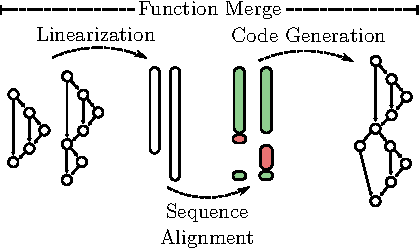
\includegraphics[width=0.85\linewidth]{src/merge-operation/figs/func-merge-overview.pdf}
  \caption{Overview of our function-merging technique.}
  \label{fig:func-merge-overview}
  %\vspace{-1ex}
\end{figure}

The proposed technique consists of three major steps, as depicted in
Figure~\ref{fig:func-merge-overview}.
First, we linearize each function, representing the CFG as a sequence of 
labels and instructions.
The second step consists in applying a sequence alignment algorithm, borrowed
from bioinformatics, which identifies regions of similarity between sequences.
The sequence alignment algorithm allows us to arrange two linearized functions
into segments that are equivalent between the two functions and segments where
they differ from one another.
The final step performs the code generation, actually merging the two functions
into a single function based on the aligned sequences.
Aligned segments with equivalent code are merged, avoiding redundancy, %redundant code,
and the remaining segments where the two functions differ have their code
guarded by a function identifier.
At this point, we also create a merged list of parameters where parameters of
the same type are shared between the functions, without necessarily keeping
their original order.
This new function can then be used to replace the original functions, as they
are semantically equivalent, given the appropriate function-identifier
parameter.

\subsection{Linearization}

The \textit{linearization}\footnote{Although linearization of CFGs
usually refers to a predicated representation, % resulting from an if-conversion,
in this paper, we refer to a simpler definition.}
of a function consits in specifying an ordering of the basic blocks based on a
traversal of the CFG and then producing a sequence of basic block labels and
instructions, similar to a textual representation of the function.
Although this operation is trivial, the specific ordering of the basic blocks
chosen can have an impact on the merging operation.

%For the linearization, we assume that every basic block has an entry label and
%a terminator instruction which refers explicitly to the successor basic blocks,
%if there are successors.
%This is true for most IRs, such as the LLVM IR, or can be easily adapted.

In our implementation, the linearization uses a reverse post-order~(RPO) of the
basic blocks, following a canonical ordering of the successors.
%, e.g., \textit{true} branches before \textit{false} ones.
%Figure~\ref{fig:branch-linearization} shows an example of the linearization 
%using the canonical RPO.
The RPO guarantees that the linearization starts with the entry basic block and
then proceeds favoring definitions before uses, except in the presence of loops.
Although the specifc ordering produced by the canonical linearization may not
be optimal, it is common practice for compilers to rely on prior
canonicalizations, e.g., 
canonical loops, canonical induction variables, canonical reassociation, etc.
For contrast, if, instead, we use an RPO linearization with a uniformly
randomized ordering of the successor basic blocks, the final code-size reduction
of the function-merging optimization can drop up to 10\% for individual
benchmarks.
Note that our decision for using the canonical RPO is purely pragmatic and
other orderings of the basic blocks could also be used, as long as it produces
a sequence of labels followed by instructions.

%\begin{figure}[h]
%  \centering
%  \includegraphics[width=0.6\linewidth]{figs/branch-linearization.pdf}
%  \caption{Linearization using a canonical reverse post-order.
%           The dashed arrows show where a randomized ordering could change the
%           linearization.}
%  \label{fig:branch-linearization}
%\end{figure}

\subsection{Sequence Alignment}

When merging two functions, the goal is to identify which pairs of instructions
and labels that can be merged and which ones need to be selected based on the
actual function being executed.
To avoid breaking the semantics of the original program, we also need to
maintain the same order of execution of the instructions for each one of
the functions.

To this end, after linearization, we reduce the problem of merging functions
to the problem of \textit{sequence alignment}. %~\cite{carrillo88,wang94}.
%After linearization, the problem of merging two functions can be reduced to the
%\textit{sequence alignment} problem~\cite{carrillo88,wang94}, which is itself
%closely related to finding the
%\textit{longest common subsequence}~\cite{hirschberg75,maier78}.
Sequence alignment is an important technique to many areas of science,
most notably in molecular biology~\cite{needleman70,smith81,carrillo88,wang94}
where, for example, it is used for identifying homologous subsequences of amino
acid in proteins.
Figure~\ref{fig:opcode-align} shows an example of the sequence alignment
between two linearized functions extracted from the \texttt{400.perlbench} benchmark
in SPEC CPU2006~\cite{spec}.

\begin{figure}[h]
  \centering
  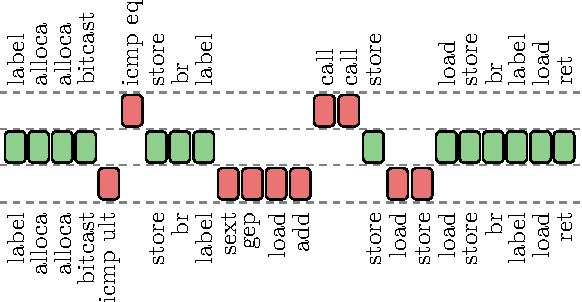
\includegraphics[width=0.85\linewidth]{src/merge-operation/figs/opcode-align.pdf}
  %\caption{An example of a sequence alignment between two real functions extracted from the \text{400.perlbench} benchmark.}
  \caption{The sequence alignment between two functions.}
  \label{fig:opcode-align}
\end{figure}

Formally, sequence alignment can be defined as follows:
For a given alphabet $\alpha$, a sequence $S$ of $k$ characters is a subset of
$\alpha^k$, i.e., $S = (a_1, \ldots a_k)$.
Let $S_1, \ldots, S_m$ be a set of sequences, possibly of different lengths but
all derived from the same alphabet $\alpha$, where
$S_i = (a_1^{(i)}, \ldots, a_{k_1}^{(i)})$, for all $i\in\{1,\ldots,m\}$.
%\begin{equation*}
%\begin{align*}
%S_1 = (a_1^{(1)}, \ldots, a_{k_1}^{(1)})\\
%\dots\\ 
%S_m = (a_1^{(m)}, \ldots, a_{k_m}^{(m)})
%\end{align*}
%\end{equation*}
Consider an extended alphabet that includes the \textit{blank} character ``$-$'',
i.e., $\beta = \alpha \cup \{-\}$.
An alignment of the $m$ sequences, $S_1, \ldots, S_m$, is another set of sequences,
$\bar{S}_1, \ldots, \bar{S}_m$, such that each sequence $\bar{S}_i$ is obtained
from $S_i$ by inserting blanks in positions where some of the other sequences
have non-blank and possibly equivalent characters, for a given equivalence relation.
All sequences $\bar{S}_i$ in the alignment set have the same length $l$, where
$\max\{k_1,\ldots,k_m\} \leq l \leq k_1 + \cdots + k_m$.
Moreover, $\forall i\in\{1,\ldots, m\}$, $\bar{S}_i = (b_1^{(i)},\ldots,b_l^{(i)})$,
there are increasing functions $v_i: \{1,\ldots,k_i\} \to \{1,\ldots,l\}$, such that:
\begin{itemize} %[noitemsep,topsep=0pt]
\item $b_{v_i(j)}^{(i)} = a_j^{(i)}$, for every $j \in \{1,\ldots,k_i\}$;
\item any position $j$ not mapped by the function $v_i$, i.e.,
for all $j \in \{1,\ldots,l\}\setminus \textrm{Im} v_i$,
then $b_j^{(i)}$ is a blank character.
\end{itemize}
Finally, for all $j\in\{1,\ldots,l\}$, there is at least one value of $i$ for
which $b_j^{(i)}$ is not a blank character.
%and for any pair of sequences that have a non-blank character at position $j$,
%these characters are equivalent.
Note that two aligned sequences may contain both non-blank and non-equivalent
characters at any given position, in which case it contains a mismatch.

Particularly for the function-merging, we are concerned with the alphabet
consisting of all possible typed instructions and labels.
Every linearized function represents a sequence derived from this alphabet.
We explain the equivalence relation used for this alphabet in the next section.

%We describe the equivalence relation between two predicated values in two
%separate cases, namely, the equivalence between instructions and the
%equivalence between labels.
%Labels are always considered equivalent.
%Two instructions are equivalent if their opcode are semantically equivalent,
%but not necessarily the same, and they both have types that can be bitcasted in
%a losslessly way from on to the other.
%This also includes making sure that there is no conflict regarding memory
%alignment when handling pointers.
%No additional restriction is imposed on the operands of the two instructions
%being compared for equivalence.
%Whenever two operands cannot be statically proved to represent the same value,
%a select instruction can be used to distinguish between the execution of two
%functions being merged.
%For function calls, the type equivalence requires that both instructions have
%identical function types, i.e., both called functions must have an identical
%return type and an identical list of parameter types. 

There is a vast literature on algorithms for performing sequence alignment,
especially in the context of molecular biology.
These algorithms range from optimal algorithms based on dynamic programming to
probabilistic models that does not guarantee
optimality~\cite{needleman70,smith81,carrillo88,hickey11}. 
In this paper, we use the Needleman-Wunsh algorithm~\cite{needleman70}.
This algorithm is based on dynamic programming and consists of two main steps.
First, it builds a \textit{similarity matrix}, based on a scoring scheme, which
assigns weights for matches, mismatches, and \textit{gaps} (blank characters).
Afterwards, a backward traversal is performed on the similarity matrix, in order
to reconstruct the final alignment by maximizing the total score.
We use a simple scoring scheme that rewards matches and penalizes mismatches and
gaps.

%\todo{Remove this paragraph.}
%When producing the final aligned sequence, there may be several possible optimal
%alignments.
%However, different aligned sequences can affect the code generation in different
%ways that may be both beneficial or undesirable. 
%For this reason, we prioritize alignments that tend to group the blank
%characters together, avoiding to frequently alternate between the two sequences
%during long segments of mismatches and gaps.
%For example, note that in Figure~\ref{fig:opcode-align}, the red blocks, for
%a particular sequence, tend to be grouped together.

\subsection{Equivalence Relation}

We describe the equivalence relation between values in two
separate cases, namely, the equivalence between instructions and the
equivalence between labels.

Labels can represent both normal basic blocks and landing blocks, which are used
in exception handling code.
Labels of normal basic blocks are always considered equivalent but
landing blocks must have exactly the same landingpad instructions.

Two instructions are equivalent if: $(1)$ their opcode are semantically
equivalent, but not necessarily the same; $(2)$ they both have equivalent types;
and $(3)$ they have pairwise operands with equivalent types.
Types are considered equivalent if they can be bitcasted in a losslessly way
from on to the other.
It is also important to make sure that there is no conflict regarding memory
alignment when handling pointers.
No additional restriction is imposed on the operands of the two instructions
being compared for equivalence.
Whenever two operands cannot be statically proved to represent the same value,
a select instruction is used to distinguish between the execution of two
functions being merged.
For function calls, the type equivalence requires that both instructions have
identical function types, i.e., both called functions must have an identical
return type and an identical list of parameter types. 

\subsubsection{Handling Exception Handling Code}

Most modern compilers implement the zero-cost Itanium ABI for exception
handling~\cite{dinechin00}, including GCC and LLVM, sometimes called the
\textit{landing-pad} model. In this section, we describe restrictions imposed
by exception handling code and their equivalence relation.

The invoke instruction co-operates tightly with its landing block, i.e., the
basic block pointed by the exception branch of an invoke instruction.
The landing block must landingpad instruction as its first non-$\phi$
instruction.
Given this restriction, two equivalent invoke instructions must also have
landing blocks with equivalent landingpad instructions.
This is easy to check since the landingpad instruction is always the first
instruction in a landing block. 

Landing blocks are responsible for handling all catch clauses of the
higher-level programming language covering the particular callsite.
All clauses are defined by the landingpad instruction, which encodes the list of
all exception and cleanup handlers.
Landingpad instructions are equivalent if they have the exactly same type and
also encode an identical lists of exception and cleanup handlers.
The type of equivalent landingpad instructions must be identical as its value
is crucial in deciding what action to take when the landing block is entered,
and corresponds to the return value of the personality function, which must also
be identical for the two functions being merged.

%The return value of the landingpad instruction is crucial in deciding what
%action to take when the landing block is entered, and corresponds to the return
%value of the personality function.

%In other words, when the unwinder executes the personality function (which
%is part of the language runtime), it stores its return value, and provides this return value in the result of the landingpad
%instruction. Since the personality function has access to the part of the unwind tables generated from the landingpad
%instruction, it can communicate information encoded in the unwind table to the landing block itself. In the libc++ runtime,
%the personality function returns a tuple consisting of a pointer to the exception object itself, and a “handler switch value”, an
%integer which corresponds to the index of a relevant “catch” clause of the landingpad instruction, or a special value (−1)
%when no catch clauses match but a cleanup needs to be performed.

%The LLVM IR generated for the landing block then checks the handler switch value computed by the personality function,
%and transfers control to a cleanup or handler block accordingly.

%Finally, if the selected handler is a cleanup handler, the
%exception propagation (stack unwinding) needs to be resumed after the cleanup is done. This is achieved by the resume
%instruction, which expects as a parameter the same value that was returned by the corresponding landingpad instruction
%which interrupted the exception propagation.
%Interestingly, there are no LLVM instructions for raising (throwing) exceptions. This is left entirely in the management
%of the language runtime, which needs to closely co-operate with the stack unwinding library anyway (the interface of the
%personality function is mandated by the stack unwinder).



%%%%%%%%%%%%%%%%%%%%%%%%%%%%%%%%%% SALSSA %%%%%%%%%%%%%%%%%%%%%%%%%%%%%%%%%%%%%%





Properly handling \textit{phi-nodes} requires a radical redesign in the code generator. The existing code generator produces code directly
from the aligned sequence, with each instruction pair treated almost in isolation without considering any control flow context. Merging
\textit{phi-nodes} cannot work with this approach because \textit{phi-nodes} are only understood in their control flow context.

\paragraph*{Road map} In the rest of this section, we describe {\ProjName}, our novel approach for merging functions through sequence alignment with full
support for the SSA form. By removing the need for preprocessing the input functions and performing register demoting, our approach is able
to merge functions better and faster. Instead of translating the aligned functions directly to merged code, the {\ProjName} follows a
top-down approach centered on the CFGs of the input functions. It iterates over the input CFGs, constructing the
CFG of the merged function, interweaving matching and non-matching instructions (Section~\ref{sec:code-gen-core}
). Afterwards, all edges and operands are resolved, including appropriately assigning the incoming values to all \textit{phi-nodes} (Section~\ref{sec:op-assign}).
{\ProjName} is designed to preserve all properties of SSA form via the standard SSA construction algorithm (Sections~\ref{sec:ssa-fix}).
Finally, {\ProjName} integrates a novel optimization with the SSA construction algorithm, called \textit{phi-node coalescing}, producing even smaller merged functions (Section~\ref{sec:pncoalescing}).

\begin{figure}[t!]
  \centering
  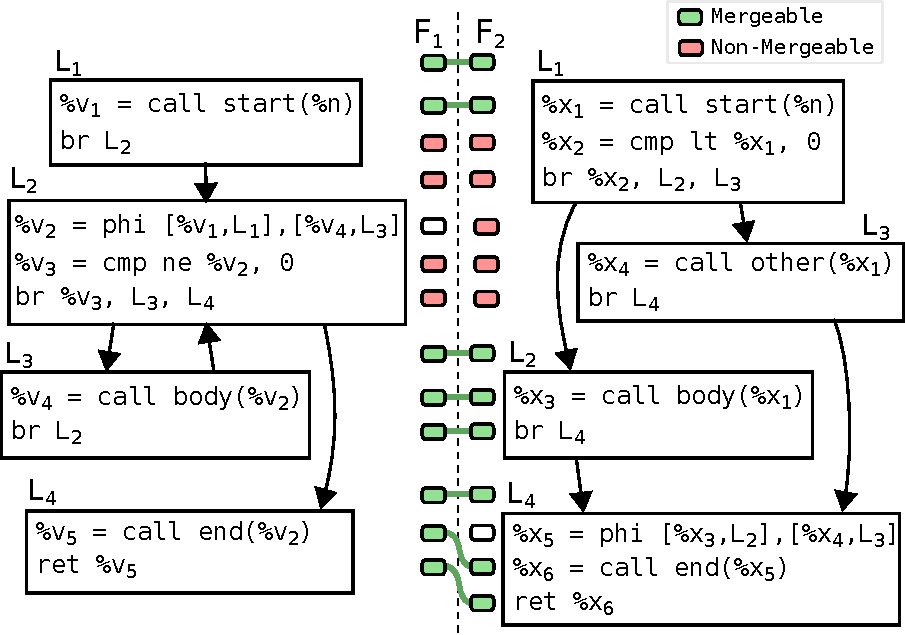
\includegraphics[scale=0.55]{src/merge-operation/figs/code-gen-cfg-input.pdf}
    \caption{Example of functions aligned without register demotion.
    \textit{Phi-nodes} are excluded from alignment.}
  \label{fig:code-gen-cfg-input}
\end{figure}

\paragraph*{Working examples} Figure~\ref{fig:code-gen-cfg-input} shows how the functions from our motivating example align without register demotion.
Here, \textit{phi-nodes} are not aligned, similarly to how FMSA handles \textit{landing-pad} instructions. We will use these as working
examples to describe step by step how our new code generator works in the next subsections.


\subsection{Control-Flow Graph Generation} \label{sec:code-gen-core}

\begin{figure}[t!]
  \centering
  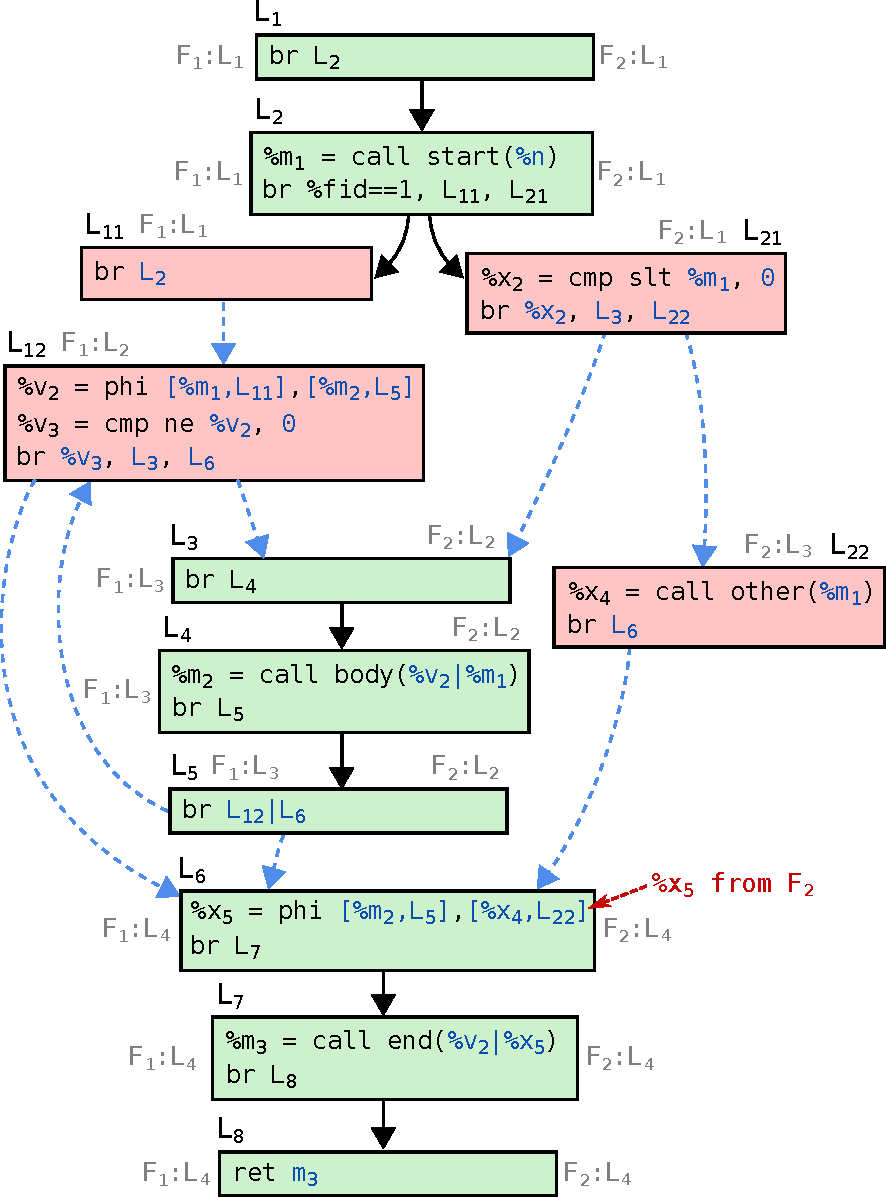
\includegraphics[scale=0.55]{src/merge-operation/figs/code-gen-cfg.pdf}
    \caption{Merged CFG produced by {\ProjName}. Code corresponding to a single
      input basic block may be transformed into a chain of blocks, separating
      matching and non-matching code. The generator inserts conditional and
      unconditional branches to maintain the same order of instructions
      from the input basic block. Operands and edges highlighted in blue will be
      resolved by the operand assignment described in Section~\ref{sec:op-assign}.}
  \label{fig:code-gen-cfg}
\end{figure}


Our code generator starts by producing all the basic blocks of the merged function.
Each original block is broken into smaller ones so that matching code is
separated from non-matching code and matching instructions and labels are placed
into their own basic blocks. Having one block per matching instruction or label
makes it easier to handle control flow and preserve the ordering of instructions
from the original functions by chaining these basic blocks as needed.

Blocks with instructions that come originally from the same basic block (of either input function) are chained in their original order with
branches. We use either unconditional branches or conditional branches on the function identifier depending on whether control flow out of
this code is different for the two input functions. Because we have one basic block per pair of matching instructions/labels, this tends to
generate some artificial branches, most of them are unconditional, but can be simplified in later stages.


%Our code generator starts by creating individual basic blocks for each pair of
%matching labels or instructions obtained from the resulting alignment.
%Afterwards, while generating the remaining and non-matching code from the input functions,
%these isolated basic blocks that represent matching code will also be chained
%together, following the order they originally appear in the input function.
%This chaining operation is performed separately for each function on a per
%basic block basis.

%For the first function, {\ProjName} iterates over each basic block, generating
%the remaining non-matching code.
%All matching and non-matching instructions generated from the same basic block
%are chained together via unconditional branches.
%As a result, each basic block from the input functions are represented by a
%sequence of basic blocks that contain either matching or non-matching
%instructions.

%Similarly, for each basic block in the second function, the non-matching
%code is generated and chained with the matching code that have already been
%generated.
%During this chaining process, if the control flow of a matching basic block
%differs from the one created for the first function,
%then {\ProjName} creates a conditional branch based on the function identifier,
%preserving the order of the instructions for both input functions.
%This process is trivial since we have the matching instructions in
%separate basic blocks and it suffices to change the branching instruction,
%selecting the correct control flow based on the function identifier.



Figure~\ref{fig:code-gen-cfg} shows the generated CFG. At this point, the only
instructions that actually have their operands assigned are the branches inserted
to chain instructions originating from the same input basic block.
These branches have no corresponding instruction in the input functions.
All other operands and edges, depicted in blue in Figure~\ref{fig:code-gen-cfg},
will be resolved later, during operand assignment.

\subsubsection{Phi-Node Generation}

Our code generator treats \textit{phi-nodes} differently from other instructions. For all alignment and code generation purposes,
{\ProjName} treats \textit{phi-nodes} as attached to their basic block's label; that is, they are aligned with their labels and are
copied to the merged function with their labels. So, when creating a basic block for a label, we also generate the \textit{phi-nodes}
associated with it. For a pair of matching labels, we copy all \textit{phi-nodes} associated with both labels.
We have decided for this approach where phi-nodes are tied to labels because phi-nodes describe primarily how data flows into its corresponding basic block.
%Figure~\ref{fig:code-gen-cfg} shows one such example, where both \textit{phi-nodes}, \texttt{v\textsubscript{2}} and
%\texttt{x\textsubscript{3}} are copied into \texttt{L\textsubscript{6}}, despite the fact it represents a pair of matching labels.
Figure~\ref{fig:code-gen-cfg} shows an example where \textit{phi-nodes} are present in basic blocks
with both matching or non-matching labels.
The phi-node \texttt{x\textsubscript{5}} is simply copied into the merged basic block labeled \texttt{L\textsubscript{6}}.

Unlike other instructions, we do not merge \textit{phi-nodes} through sequence alignment.
Instead, identical \textit{phi-nodes} are merged during the simplification process
using existing optimizations from LLVM.
%LLVM provides an optimization for eliminating identical \textit{phi-nodes} which
%we apply later to clean-up the code.

\subsubsection{Value Tracking}

While generating the basic blocks and instructions for the merged function,
{\ProjName} keeps track of two mappings that will be needed during operand assignment.
The first one, called \textit{value mapping}, is responsible for mapping labels
and instructions from the input functions into their corresponding ones in the merged
function.
This is essential for correctly mapping the operand values.
The second one, called \textit{block mapping}, is a mapping of the basic blocks
in the opposite direction, as shown by the light gray labels in Figure~\ref{fig:code-gen-cfg}.
It maps basic blocks in the merged function to a basic block in each input functions,
whenever there is a corresponding one.
This \textit{block mapping} will be needed to map control flow when assigning the
incoming values of \textit{phi-nodes} (see Section~\ref{sec:phi-in-vals}).

\subsection{Operand Assignment} \label{sec:op-assign}

Once all instructions and basic blocks have been created, we perform operand
assignment in two phases.
First, we assign all label operands, essentially resolving the remaining edges
in the control flow graph (dashed blue edges in Figure~\ref{fig:code-gen-cfg}).
With the control flow graph complete, we can then create a dominator
tree to help us assign the remaining operands while also properly
handling instruction domination.

\begin{figure}[t]
  \centering
  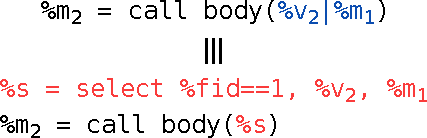
\includegraphics[scale=0.7]{src/merge-operation/figs/operand-select.pdf}
  \caption{Operand selection for the \texttt{call} instruction in \texttt{L\textsubscript{4}}
             from Figure~\ref{fig:code-gen-cfg}. Mismatching operands chosen
             with a \texttt{select} instruction on the function identifier.}
  \label{fig:operand-select}
\end{figure}

Whenever the corresponding operands of merged instructions are different, we
need a way to select the correct operand based on the function identifier.
Section~\ref{sec:label-select} describes how we perform label selection.
In all other cases, we simply use a \textit{select} instruction, as shown in
Figure~\ref{fig:operand-select}.

\begin{figure}[t]
  \centering
  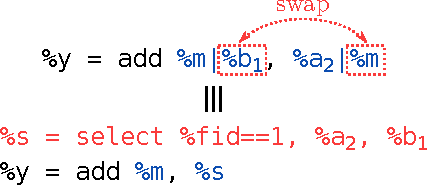
\includegraphics[scale=0.7]{src/merge-operation/figs/operand-select-reorder.pdf}
    \caption{Optimizing operand assignment for commutative instructions.
             Example of a merged \texttt{add} instruction that can have its
             operands reordered to allow merging the two uses of \texttt{\%m},
             avoiding a \textit{select} instruction.}
  \label{fig:operand-select-reorder}
\end{figure}

When assigning operands to commutative instructions, we also perform operand
reordering to maximize the number of matching operands and reduce the need for
\textit{select} instructions.
Figure~\ref{fig:operand-select-reorder} shows an example of a commutative instruction
where an operand selection can be avoided by reordering operands.
%This property of commutative operations has been exploited before by other
%optimizations~\cite{porpodas18a,porpodas19,rocha19}.

\subsubsection{Label Selection} \label{sec:label-select}

In LLVM, labels are used exclusively to represent control flow.
More specifically, label operands are used by terminator instructions, where
they specify the destination basic block of a control flow transfer, or
to represent incoming control flow in a \textit{phi-node} instruction.

Whenever assigning the operands of a merged terminator instruction, if there is
a label mismatch between the two input functions, we need a way to select
between the two labels depending on the executed function.
We do so by creating a new basic block with a conditional branch on the function
identifier to each one of the mapped labels. Then we use the new block's label as
the operand of the merged terminator instruction.
Figure~\ref{fig:label-select} illustrates a CFG that handles label selection for
a merged terminator instruction.

\begin{figure}[t]
  \centering
  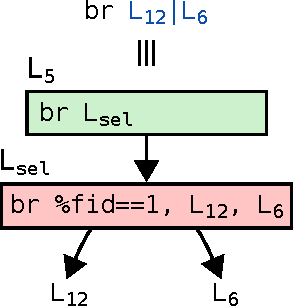
\includegraphics[scale=0.65]{src/merge-operation/figs/label-select.pdf}
  \caption{Label selection for mismatched terminator instruction operands
	\texttt{L\textsubscript{f1}} and \texttt{L\textsubscript{f2}} corresponding
	to labels of two different basic blocks. We handle control flow in a new
	basic block, \texttt{L\textsubscript{sel}} with a conditional branch on the
	function identifier targeting the two labels. We use the label of the new
	block as the merged terminator operand.}
  \label{fig:label-select}
\end{figure}

\subsubsection{Landing Blocks}

Most modern compilers, including GCC and LLVM, implement the zero-cost Itanium ABI for exception handling~\cite{dinechin00}, which is known
as the \textit{landing-pad} model. This model has two main components: $(1)$ invoke instructions that have two successors, one that
continues when the call succeeds as per normal, and another, usually called the \textit{landing pad}, in case the call raises an exception,
either by a throw or the unwinding of a throw; $(2)$ landing-pad instructions that encode which action is taken when an exception is
raised. A landing pad must be the immediate successor of an invoke instruction in its unwinding path. The code generator must ensure that
this model is preserved.

Our new code generator delays the creation of landing-pad instruction until
the phase of operand assignment.
Once we have concluded the remapping of all label operands of an invoke instruction,
regardless of whether they are merged or non-merged code, we create an
intermediate basic block with the appropriate landing-pad instruction.
Then we assign the label of this landing block as the operand of
the invoke instruction, as shown in Figure~\ref{fig:landingpad}.

\begin{figure}[t!]
  \centering
  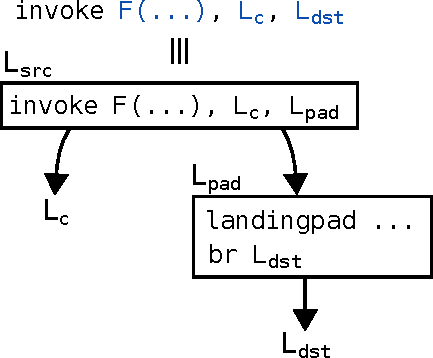
\includegraphics[scale=0.65]{src/merge-operation/figs/landingpad.pdf}
  \caption{Landing blocks are added after operand assignment and
	are assigned to invoke instructions as operands.}
  %\fixme{PP: not sure whether this plot is interesting.}
  \label{fig:landingpad}
\end{figure}

\subsubsection{Phi-Node's Incoming Values} \label{sec:phi-in-vals}

There are two distinct cases for \textit{phi-nodes}: being associated with a
matching or with a non-matching label. In both cases, \textit{phi-nodes} are
only copied from their input functions and they are not merged. So each
\textit{phi-node} in the merged function should capture the incoming flows
present in the corresponding \textit{phi-node} of their input function. For
matching labels, each \textit{phi-node} in the merged function will have
additional incoming flows specific to the \textit{other} input function but
these flows should have undefined values.

To assign the incoming values of a \textit{phi-node}, {\ProjName} iterates over
all predecessors of its parent basic block and uses the \textit{block mapping}
to discover each predecessor's corresponding basic block in the input function.
If such a basic block is found, then
{\ProjName} obtains the incoming value associated with that predecessor from the \textit{value mapping}.
Otherwise, an undefined value, which by construction should never be actually used,
is associated with that predecessor.

\subsection{Preserving the Dominance Property} \label{sec:ssa-fix}
%
%After code generation, {\ProjName} ends up with a code that violates the
%\textit{dominance property} of the SSA form.
The code transformation process described so far could violate the \textit{dominance property} of the SSA form. This property states that
each use of a value must be dominated by its definition. For example, an instruction (or basic block) dominates another if and only if
every path from the entry of the function to the latter goes through the former. Figure~\ref{fig:phi-placement-1} gives one example
extracted from Figure~\ref{fig:code-gen-cfg} where the the dominance property is violated during code transformation.

\begin{figure}[t]
  \centering
  \begin{subfigure}{.5\textwidth}
    \center
    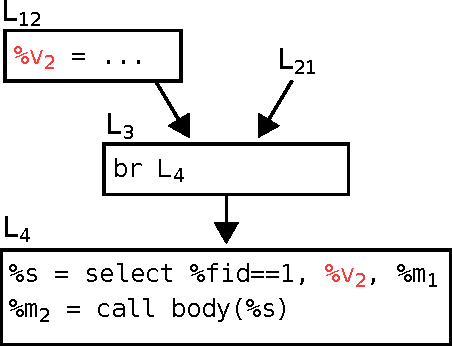
\includegraphics[scale=0.65]{src/merge-operation/figs/phi-placement-1}
    \caption{Example where the dominance property is violated.}
    \label{fig:phi-placement-1}
  \end{subfigure}
  \\
  \begin{subfigure}{.5\textwidth}
    \center
    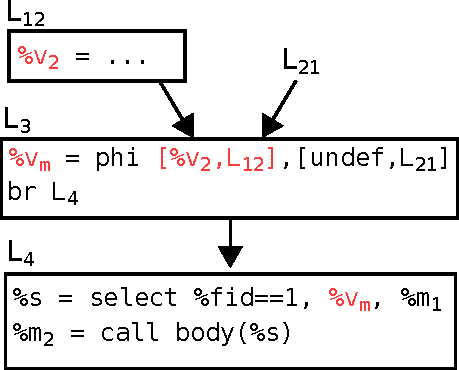
\includegraphics[scale=0.65]{src/merge-operation/figs/phi-placement-2}
    \caption{The dominance property is restored by placing phi-nodes where needed.}
    \label{fig:phi-placement-2}
  \end{subfigure}
  \caption{Example of how {\ProjName} uses the standard SSA construction algorithm
           to guarantee the dominance property of the SSA form.}
  \label{fig:phi-placement}
\end{figure}


%The dominance property states that each use of a value must be dominated by its definition. An instruction (or basic block) dominates
%another if and only if every path from the entry of the function to the latter goes through the former. Figure~\ref{fig:phi-placement-1}
%shows one small example extracted from Figure~\ref{fig:code-gen-cfg} that illustrates a violation of the dominance property. {\ProjName}
%restores this property by first adding a \textit{pseudo-definition} at the entry block of the function where names are defined and
%initialized with an \textit{undefined} value. This guarantees that every register name will be defined on basic blocks from both functions.
%Then, {\ProjName} applies the standard SSA construction algorithm~\cite{cytron89,cytron91}, which guarantees both the dominance and the
%single-reaching definition properties of the SSA form. Figure~\ref{fig:phi-placement-2} shows the resulting code.




{\ProjName} is designed to preserve the dominance property to conform with the SSA form.
It achieves this using a two-step approach.
It first adds a \textit{pseudo-definition} at the entry block of the function where names are defined and initialized with an
\textit{undefined} value.
This guarantees that every register name will be defined on basic blocks from both functions.
Then, {\ProjName} applies the standard SSA construction algorithm~\cite{cytron89,cytron91}, which guarantees both the dominance and the
single-reaching definition properties of the SSA form.
We note that our implementation uses the standard SSA construction algorithm provided by LLVM for register promotion.
This algorithm guarantees that names have a single definition by placing extra phi-nodes where needed so that instructions can be renamed appropriately.
Figure~\ref{fig:phi-placement-2} shows how the property violation in Figure~\ref{fig:phi-placement-1} can be corrected using this strategy.

%Formally, this algorithm can be described as follows.
%Given a set of definitions to the same name, the placement of phi-nodes consists of computing its \textit{iterated dominance frontier}, as define below:

%\begin{definition}[Dominance Frontier]
%The \textit{dominance frontier} of a node $n$, $DF(n)$, is the set of all nodes $n'$
%such that $n$ dominates an \textit{immediate} predecessor of $n'$ but does not \textit{strictly} dominate $n'$.
%This definition also extends to sets of nodes.
%The \textit{dominance frontier} of a set of nodes $S$ is the union of each \textit{dominance frontier},
%i.e., $DF(S) = \bigcup_{n\in S}DF(n)$.
%\end{definition}

%\begin{definition}[Iterated Dominance Frontier]
%The \textit{iterated dominance frontier} of a set of nodes $S$ is the limit $DF^+_{i\to\infty}(S)$ of the recurrence equation below:
%\begin{align*}
%DF^+_1(S) &= DF(S) \\
%DF^+_{i+1}(S) &= DF(S\cup DF^+_i(S))
%\end{align*}
%\end{definition}

%Given a register name $v$, phi-nodes are placed in all basic blocks from set $DF^+(Defs(n))$, where $Defs(v)$ is the set of all basic
%blocks, which contains a definition of $v$. For the example shown in Figure~\ref{fig:phi-placement}, we have
%$Defs(\texttt{\%v\textsubscript{2}}) = \{ \texttt{L\textsubscript{12}}, \texttt{L\textsubscript{1}} \}$, where the entry block
%\texttt{L\textsubscript{1}} contains the \textit{pseudo-definition}.

%%%
%%%Although this is enough to guarantee the correctness of the SSA form,
%%%there are still optimization opportunities that can be explored by {\ProjName}.
%%%We discuss these opportunities for optimization in the next section.

\subsection{Phi-Node Coalescing} \label{sec:pncoalescing}

The approach described in Section~\ref{sec:ssa-fix} guarantees the correctness of the SSA form but generates extra
phi-nodes and registers which increase register pressure and might lead to more \textit{spill code}. In this section, we describe a novel optimization technique, \textit{phi-node coalescing}, that {\ProjName} uses to lower register pressure.

%The approach described in Section~\ref{sec:ssa-fix} guarantees the correctness of the SSA form but leaves room for improvement.
%In this section, we describe \textit{phi-node coalescing}, a novel optimization technique employed by {\ProjName} to lower the register
%pressure on the final merged code by reducing the number of phi-nodes required.
%This reduces code size of the merged function since a lower register pressure allows the register allocator to produce fewer \textit{spill code}.

Figure~\ref{fig:phi-coalescing-select} illustrates such an optimization opportunity. {\ProjName} is merging an instruction with different arguments,
so it needs to select the right one based on the function identifier. The two arguments though, \texttt{v} and \texttt{x}, have \textit{disjoint definitions},
i.e. they have non-merged definitions from different input functions. Using the standard SSA construction algorithm would result in
the sub-optimal code shown in Figure~\ref{fig:phi-coalescing-select-1}. This code inserts two trivial phi-nodes to select, again, \texttt{v} or \texttt{x}
based on the executed function. {\ProjName} optimizes this code by coalescing both phi-nodes into a single one and removing the
selection statement. As shown in Figure~\ref{fig:phi-coalescing-select-2}, the optimized version has a smaller number of instructions and
phi-nodes.


%This example contains a pair of \textit{disjoint
%definitions} \texttt{v} and \texttt{x}, i.e. two non-merged definitions that came originally from different input functions. This pair of
%disjoint definitions is used via a selection in a merged instruction. Simply using the standard SSA construction algorithm would result in
%the sub-optimal code shown in Figure~\ref{fig:phi-coalescing-select-1}. This code has two trivial phi-nodes, one for the definition in each
%function, and a final selection. {\ProjName} further optimizes this code by coalescing both phi-nodes into a single one, removing the
%selection statement. As shown in Figure~\ref{fig:phi-coalescing-select-2}, the optimized version has a smaller number of instructions and
%phi-nodes.

\begin{figure}[t]
  \centering
  \begin{subfigure}{.5\textwidth}
    \center
    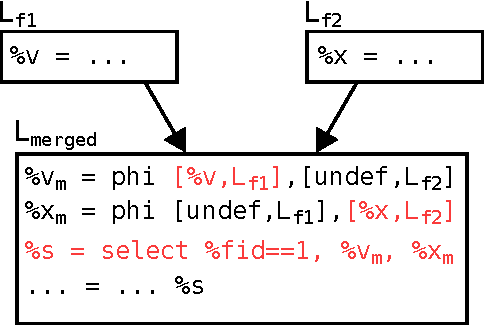
\includegraphics[scale=0.65]{src/merge-operation/figs/phi-coalescing-select-1}
    \caption{Phi-node placement without coalescing.}
    \label{fig:phi-coalescing-select-1}
  \end{subfigure}
  \\
  \begin{subfigure}{.5\textwidth}
    \center
    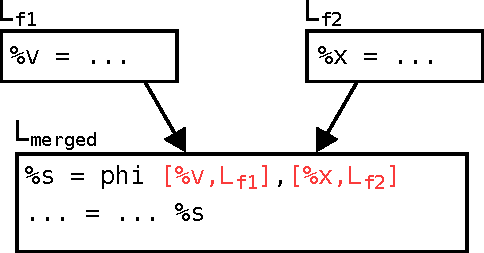
\includegraphics[scale=0.65]{src/merge-operation/figs/phi-coalescing-select-2}
    \caption{Phi-node placement with coalescing.}
    \label{fig:phi-coalescing-select-2}
  \end{subfigure}
  \caption{Phi-node coalescing reduces the number of phi-nodes and selections.}
  \label{fig:phi-coalescing-select}
\end{figure}

\begin{figure}[h]
  \centering
  \begin{subfigure}{.5\textwidth}
    \center
    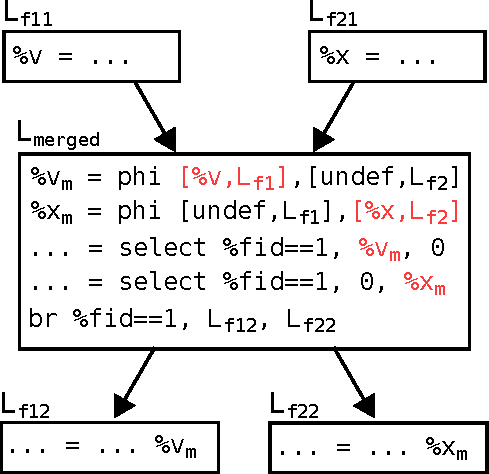
\includegraphics[scale=0.65]{src/merge-operation/figs/phi-coalescing-gen-1}
    \caption{Phi-node placement without coalescing.}
    \label{fig:phi-coalescing-gen-1}
  \end{subfigure}
  \\
  \begin{subfigure}{.5\textwidth}
    \center
    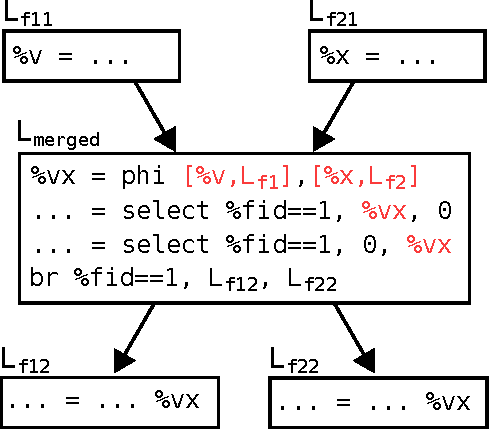
\includegraphics[scale=0.65]{src/merge-operation/figs/phi-coalescing-gen-2}
    \caption{Phi-node placement with coalescing.}
    \label{fig:phi-coalescing-gen-2}
  \end{subfigure}
  \caption{Reducing the number of phi-nodes by coalescing disjoint definitions with no user instructions
in common.}
  \label{fig:phi-coalescing-gen}
\end{figure}

This transformation is valid because a value definition that
is exclusive to a function will never be used when executing
the other function.
Figure~\ref{fig:phi-coalescing-gen} shows another example
illustrating that even disjoint definitions that have no user instructions
in common can be coalesced, reducing the number of phi-nodes.

Since {\ProjName} is aware of which basic blocks are exclusive to each function, it can choose a pair of disjoint definitions for
coalescing. Given a pair of disjoint definitions, {\ProjName} assigns the same name for both of them before applying the SSA
reconstruction. {\ProjName} coalesces the set of definitions that violate the dominance property. Two definitions can be paired for
coalescing if they are disjoint and have the same type. The optimization pairs disjoint definitions that maximize their live range overlap
since the goal is to avoid having register names live longer than they should, reducing register pressure.

Formally, the heuristic implemented in our phi-node coalescing can be described as follows:
Given a set $S_1\times S_2$ of disjoint definitions that violate the dominance property,
the optimization chooses pairs $(d_1,d_2)\in S_1\times S_2$ that maximize the intersection $U\!B(d_1)\cap U\!B(d_2)$,
where $U\!B(d)$ is the set \text{$\{ Block(u) : u\in Users(d) \}$}.

Phi-node coalescing allows {\ProjName} to produce smaller merged functions and reduce code size.
Consequently, it also enables more functions to be profitably merged.


\chapter{Function Merging by Sequence Alignment} \label{chp:cgo19}

In this chapter, we present our novel function merging technique.
Our approach is based upon the concept of sequence alignment, developed in
bioinformatics for identifying functional or evolutionary relationships between
different DNA or RNA sequences. Similarly, we use sequence alignment to find
areas of functional similarity in arbitrary function pairs. Aligned segments
with equivalent code are merged. The remaining segments where the two functions
differ are added to the new function too but have their code guarded by a
function identifier. This approach leads to significant code size reduction.

Applying sequence alignment to all pairs of functions is prohibitively expensive
even for medium sized programs. To counter this, our technique is integrated with
a ranking-based exploration mechanism that efficiently focuses the search to the most
promising pairs of functions. %\todo{whats interesting about this ranking?}.
As a result, we achieve our code size savings while introducing little compilation-time
overhead.

Compared to identical function merging, we introduce extra code to be executed,
namely the code that chooses between dissimilar sequences in merged functions.
A naive implementation could easily hurt performance, e.g by merging two hot functions
with only few similarities. Our implementation can avoid this by incorporating
profiling information to identify blocks of hot code and effectively minimize 
the overhead in this portion of the code.
%disable code size optimizations for them. 

In this chapter, we make the following contributions:
\begin{itemize}
  \item We are the first to allow merging arbitrary functions, even ones with
    different signatures and CFGs.
  \item A novel ranking mechanism for focusing inter-procedural optimizations
    to the most profitable function pairs.
  \item Our function merging by sequence alignment technique is able to reduce
     code size by up to 25\% on Intel and 30\% on ARM, significantly outperforming the
    state-of-the-art, while introducing minimal compile-time and negligible run-time overheads.
\end{itemize}

\section{Background and Motivation} \label{sec:motivation}

%In this section, we discuss the key weaknesses of the state-of-the-art function merging, called {\SOAName}~\cite{rocha20}, addressed in this paper.
%First, we show how different stages in {\SOAName} impact its running time.
%\textbf{TODO: Memory usage.}

%In this section, we will discuss how different stages of the state-of-the-art function merging impact during compilation time.
%present how different stages of the state-of-the-art function merging impact its running time.
%In this section, we will present how sequence alignment can be an important source of compilation time overhead.
%Then we discuss how we can address this issue by doing less work, while still keeping most of the code size reduction from the state-of-the-art technique.

In this section, we first provide an overview of the working mechanism of \SOAName, described in Chapter~\ref{chp:pldi20}. We highlight the main drawbacks of \SOAName in terms of compile time and memory footprint. We then outline how we can address these drawbacks without compromising on code size reduction. 

\subsection{Function Merging via Sequence Alignment}
Existing function merging techniques consist of three major stages: choosing which functions to merge, producing the merged function, and estimating the merging profitability.
%\fixme{PP: Is it accurate to talk about two major stages in SalSSA and also this being the case for most optimizations?}

In order to pair similar functions for merging, \SOAName employs a ranking strategy based on the similarity of the \textit{fingerprints} of the functions.
A fingerprint summarizes the content of a function as a fixed-size vector of the frequency of each LLVM-IR opcode. The representation allows the compiler to compare functions using a simple distance metric, such as the Manhattan distance. For a given reference function, all other functions are ranked based on their distance and the closest function is chosen for merging.

Merging two functions requires identifying similar code segments in the two functions that can be profitably merged.
The main innovation of \SOAName~\cite{rocha20} and its predecessor~\cite{rocha19} is the use of a sequence alignment algorithm, called the \NW algorithm, for identifying similar code segments.
This allows them to merge arbitrary pairs of functions.
First, they transform each function into a linear sequence of labels and instructions.
Then, the alignment algorithm is applied on the sequences of the whole input functions.
The resulting alignment is used to generate the merged function.
Once the merged function has been generated, they apply an SSA reconstruction algorithm.
For a final clean up, they simplify the merged function by removing redundant instructions introduced by function merging.
% PP: still not sure that this information is useful for understanding our contribution

Finally, a profitability analysis estimates the benefit of replacing the original pair of functions with the simplified merged function. If unprofitable, the merged function is simply thrown away. Otherwise, they delete the original functions, redirecting the calls to the merged function.
%If the original functions cannot be deleted, e.g., because they might be called externally, their body is replaced by a call to the merged function.
% PP: Similarly not really important for understanding our contribution

\subsection{Limitations of The State of The Art}
%PP: I think we should reorganise this a bit. After refocusing the discussion here on memory, jumping to a subsection called "Compilation Overhead Breakdown" that mainly talks about compilation time seems disconnected. Instead, we should merge the two subsection making the first half about the limitations in terms of memory and the second about the limitations in terms of runtime.

When reproducing the {\SOAName} experiments using the available artifact~\cite{rocha20} on our machine, we were unable to build \texttt{602.gcc\_s}, from SPEC 2017, due to an out of memory crash. 16~GB of memory were not enough for {\SOAName}. 
We succeeded only after migrating to a 64~GB machine which could fit the 32~GB of temporary data produced by function merging.
After investigating further, we realized that this is due to the quadratic algorithm used for aligning the two functions selected for merging.
Because this algorithm is applied on the linearized sequences of the whole input functions, \SOAName incurs a high memory footprint when merging even medium sized functions.
For larger ones, it is impossible to apply it on most workstations or even many servers, making {\SOAName} impractical for use in production.
%For the same reason, alignment brings the compilation process to a crawl for large functions.


%\subsection{Compilation Overhead Breakdown}
\label{sec:motivation:breakdown}

%When merging two functions, the goal is to identify which segments of the code are different and which ones are equivalent, and therefore mergeable.
%To this end, SalSSA uses an optimal sequence alignment algorithm, called the Needleman-Wunsch algorithm, which is quadratic on the size of the input sequences.
%Since SalSSA applies it on the linearised sequences of the whole input functions, the time spend aligning sequences can be significant for programs with very large functions.

For the same reason, alignment brings the compilation process to a crawl for large functions.
Figure~\ref{fig:compilation-breakdown-motivation-alignment} shows the running time breakdown for the different stages of the function merging pass in the LLVM-based \SOAName  implementation for two SPEC CPU2017 benchmarks. 
Sequence alignment dominates the running time of function merging, representing up to 83\% of its overall running time. 
Sequence alignment alone takes 25 seconds and 4.2 minutes on \texttt{638.imagick\_s} and \texttt{602.gcc\_s}, respectively.
%PP: Remove the next sentence?
The alignment stage also causes the peak in memory usage for these two programs, 4.5~GB for \texttt{638.imagick\_s} and 32~GB for \texttt{602.gcc\_s}.
This is not surprising, as the Needleman-Wunsch algorithm has a quadratic complexity in both time and memory usage.
Because this algorithm is applied on linearized sequences of the whole input functions, programs containing large functions, such as the ones in our example, are heavily affected.
%For example, \texttt{638.imagick\_s} has a total of 15,454 functions with the largest one having 73,127 instructions.
%Meanwhile, even though \texttt{602.gcc\_s} has only 2,457 functions, its largest function has 28,974 instructions; hence \SOAName also incurs significant peak memory usage when processing this program. 

\begin{figure}[h]
  \centering
  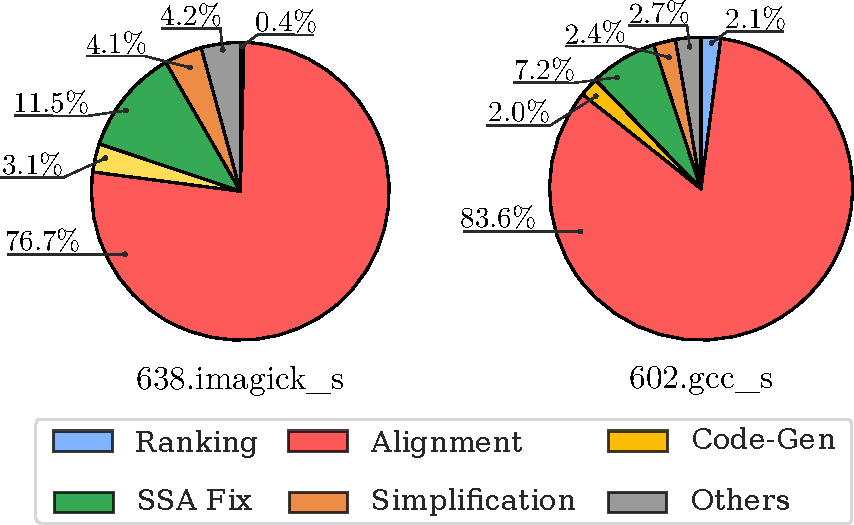
\includegraphics[width=0.7\linewidth]{src/lctes21/figs/compilation-breakdown-motivation-alignment.pdf}
  \caption{Breakdown of the relative runtime for the different stages from {\SOAName}. Alignment takes 25 seconds and 4.2 minutes on \texttt{638.imagick\_s} and \texttt{602.gcc\_s}, respectively.}
  \label{fig:compilation-breakdown-motivation-alignment}
\end{figure}

Most of the rest of the running time of function merging is associated with producing merged functions from the aligned sequences.
%\fixme{PP: Same suggestion as earlier about CodeGen.}
This includes the time spent on the code generation stage (Code-Gen), SSA reconstruction (SSA Fix), and code simplification (Simplification). These stages account for 18.7\% of the {\SOAName}’s running time on \texttt{638.imagick\_s} and 11.6\% on \texttt{602.gcc\_s}.
However, for other programs, these stages may represent the vast majority of {\SOAName}’s running time (see Section~\ref{sec:eval:pass-speedup}).

This breakdown includes the cost for producing both \emph{profitable} and \emph{unprofitable} merged functions.
In fact, most of it is wasted on merged functions that will be rejected by the profitability analysis.
These costs are pronounced because unprofitably merged functions have no limit on their size or complexity, often adding a significant pressure on the SSA reconstruction and simplification stages.
This effect is tied to the alignment strategy, since a good alignment is needed for producing profitably merged functions.
As we discuss in Section~\ref{sec:motivation:less-more}, a better approach would include a finer grain profitability analysis that would allows us to bail out from merging complex and unprofitable code as early as possible.

\subsection{When Less is More} \label{sec:motivation:less-more}

We observe that most of the benefit of function merging often comes from merging highly similar, but not necessarily identical, basic blocks. Figure~\ref{fig:xalan-example} shows one such example extracted from the \texttt{483.xalancbmk} benchmark found in SPEC CPU2006.
This example shows the two input functions annotated with the alignment produced by \SOAName. Merging these two functions contributes to a reduction of 33 bytes in the final object file.

\begin{figure}[h]
  \centering
  \includegraphics[width=\linewidth]{src/lctes21/figs/xalan-example.pdf}
  \caption{Example extracted from \texttt{483.xalancbmk} in SPEC CPU2006. Instructions marked green have been aligned through sequence alignment with an instruction from the other function. {\SOAName} would attempt merging all matched instructions but only the ones in fully aligned basic blocks would be profitable.}
  \label{fig:xalan-example}
\end{figure}

% \begin{figure*}[h]
%   \centering
%   \includegraphics[width=0.6\textwidth]{figs/xalan-example.pdf}
%   \caption{Example extracted from \texttt{483.xalancbmk} found in SPEC CPU2006.}
%   \label{fig:xalan-example}
% \end{figure*}

%This example also suggests that 
While this approach is flexible enough to identify very complex alignments, what it actually produces is three aligned pairs of basic blocks and a few aligned instructions in the entry blocks. More importantly, these entry block instructions offer nothing in terms of code size reduction. The gains of merging them are negated by the extra branches and operand selections needed to preserve the program's semantics. Since {\SOAName} analyzes the profitability of the final merged function as a whole, this unprofitable sequence of instructions will be merged because of the three highly profitable basic blocks. For the same reason, we may have profitable areas of code rejected because the rest of the merged function is unprofitable.


%Since {\SOAName} analyzes the profitability of the final merged function as a whole, we may have segments of unprofitably merged code inside an otherwise profitably merged function.
%Similarly, we may also have segments of profitably merged code inside merged functions that are thrown away by the profitability analysis. 
%However, we can achieve the same code size reduction of 33 bytes by merging only the subset of nearly identical basic blocks (highlighted in Figure~\ref{fig:xalan-example}).
%The gains of merging the entry blocks are negated by the extra branches and operand selections needed to preserve the program's semantics.

This example shows us that we could achieve similar code size reduction by breaking the problem of aligning functions into two simpler processes: first identifying highly similar basic blocks and then aligning the instructions in each pair of similar blocks. 
%merging functions on the basic block rather than on the instruction level adopted by \SOAName.
By operating on basic blocks, we could greatly reduce the length of the sequences to be aligned and the associated compilation and memory overhead. Furthermore, by making profitability decisions for each pair of basic blocks separately, we could avoid merging unprofitable pairs. The rest of this chapter shows how we use such an approach to overcome the weaknesses of \SOAName and make function merging practical for optimizing large programs. 

%Therefore, the main takeaways are:
%1) It often suffices to merge functions on a per basic block manner. %, since crossing the basic block boundary is rarely necessary.
%2) A fine-grain profitability analysis is needed to avoid  merging unprofitable pairs of basic blocks.



%This happens because the optimal sequence alignment algorithm used by SalSSA is trying to maximize the number of matching entries, which does not necessarily translate to the optimal merged function.
%Moreover, SalSSA is also limited by the fixed linearization strategy.
%For example, the two \textit{return} instructions are not aligned due to the ordering of the basic blocks chosen by the linearization strategy.

%We can take advantage of this insight in order to design a faster function merging technique.
%Ultimately, our goal is to be able to avoid the quadratic algorithm while still producing significant reductions to the program's size.

%In this paper, we take advantage of these key insights to propose a novel function merging technique that addresses the major overheads discussed in Section~\ref{sec:motivation:breakdown}.
%We can take advantage of this insight in order to design a better and faster function merging technique.
%To this end, we propose a novel function merging technique that work on the level of basic blocks and includes a fine-grain profitability analysis.



%bail out early from   of a fine-grain and a coarse-grain analysis.

%TODO: [Relatedwork] Note that this is different from the work done by von Koch~et~al.~\cite{edler14}, as these two functions are not \textit{structurally similar} as expected by their function merging technique and therefore could not be merged.


\input{src/cgo19/proposed}
\section{Evaluation}
\label{sec:evaluation}

In this section, we compare {\ProjName} against {\SOAName}, presented in Chapter~\ref{chp:pldi20}.
First, we evaluate the code size reduction achieved by each technique, demonstrating that our approach is on a par with {\SOAName}. Then we show that {\ProjName} reduces significantly the overhead of function merging. % to such a degree that it becomes negligible.
Combined with the speedup in later stages of the compilation pipeline due to the reduced amount of code, {\ProjName} leads to faster end-to-end compilation than a baseline with no function merging enabled. Finally, we demonstrate how our contributions reduce the memory usage by several orders of magnitude. 

\subsection{Experimental Setup}
%We compare {\ProjName}, our novel function merging technique, against {\SOAName}, the  state-of-the-art~\cite{rocha20}.
In addition to evaluating \SOAName, we also consider four variations of our technique based on two dimensions:
1) the linear Pairwise Alignment (PA) versus the quadratic {\NW} Alignment (NW), both on a per basic block manner and
2) using a multi-tier profitability analysis versus using only the standard profitability analysis from {\SOAName}, which is the analysis applied on the whole function after generating the merged function.
As described in Section~\ref{sec:contribution}, the [PA] variant is, by construction, limited to merging only basic blocks of the same size. The [NW] variant can merge blocks of different sizes. The four variations are:

\begin{itemize}
    \item {[PA]}: PA with the Multi-tier Profitability analysis.
    \item {[PA,NMP]}: PA with No Multi-tier Profitability.
    \item {[NW]}: NW with the Multi-tier Profitability.
    \item {[NW,NMP]}: NW with No Multi-tier Profitability.
    %\item {[NW,SS]}: NW with Block Profitability but applied on blocks of the Same Size (SS).
\end{itemize}

%For \SOAName, we used the version published in their evaluation artifact~\cite{SalSSA}.
To keep the comparison fair, we implemented {\ProjName} for the same compiler as \SOAName, LLVM \fixme{v11}. We evaluated all techniques on the C/C++ programs from the SPEC CPU 2006 and the SPEC CPU 2017 benchmark suites~\cite{spec}. The baseline in all cases is the LLVM build in full LTO mode without any function merging.

We target the Intel x86 architecture.
All experiments were performed on a dedicated server with a quad-core Intel Xeon CPU E5-2650, 64 GiB of RAM, running Ubuntu 18.04.3 LTS. To minimize the effect of measurement noise, we repeated all compilation and runtime overhead experiments 5 times. We report the average values and their 95\% confidence intervals.

We evaluate all approaches in terms of code size reduction, time overhead of function merging, end-to-end compilation time, and peak memory usage. To better examine the trade-off between code size reduction and compilation time, we also introduce and measure a new metric called \textit{average reduction speed} which shows the efficiency of the optimization at reducing code size. This metric offers a single number that allows us to compare how different versions address the trade-off between compilation time and code size reduction.

\begin{definition}[Average Reduction Speed]
For a given input program and optimization, let $S$ and $S_0$ be the size of the program with and without the given optimization, respectively.
$R = S_0 - S$ represents the reduction achieved by such optimization.
Let $T$ be the running time of the optimization pass.
We define the \textit{average reduction speed} as:
\[
   ARS = \frac{R}{T}
\]  
\end{definition}

\subsection{Code Size Reduction} \label{sec:eval:size}

Figures~\ref{fig:size-reduction-both} reports the reduction on the size of the linked object files produced by the compiler.
While limiting alignment at a basic block granularity seems restrictive, its effect on code size is small. Even the worst performing variants of {\ProjName} are still within 3 percentage points of {\SOAName}, while both [PA] and [NW] achieve good results that are on a par with {\SOAName}. [PA]'s code size reduction varies from 5 percentage points worse to over 10 points better than {\SOAName}. On average, it is within 1 percentage point of the reduction achieved by {\SOAName}. [NW] almost always achieves better code size reduction than [PA] and on average outperforms {\SOAName} by a small margin. Since our primary aim is to reduce the high compile-time overheads of {\SOAName}
%, in the following sections,
a small loss of code reduction is acceptable. 

 \begin{figure}[h]
   \centering
 \begin{subfigure}{\textwidth}
 \center
   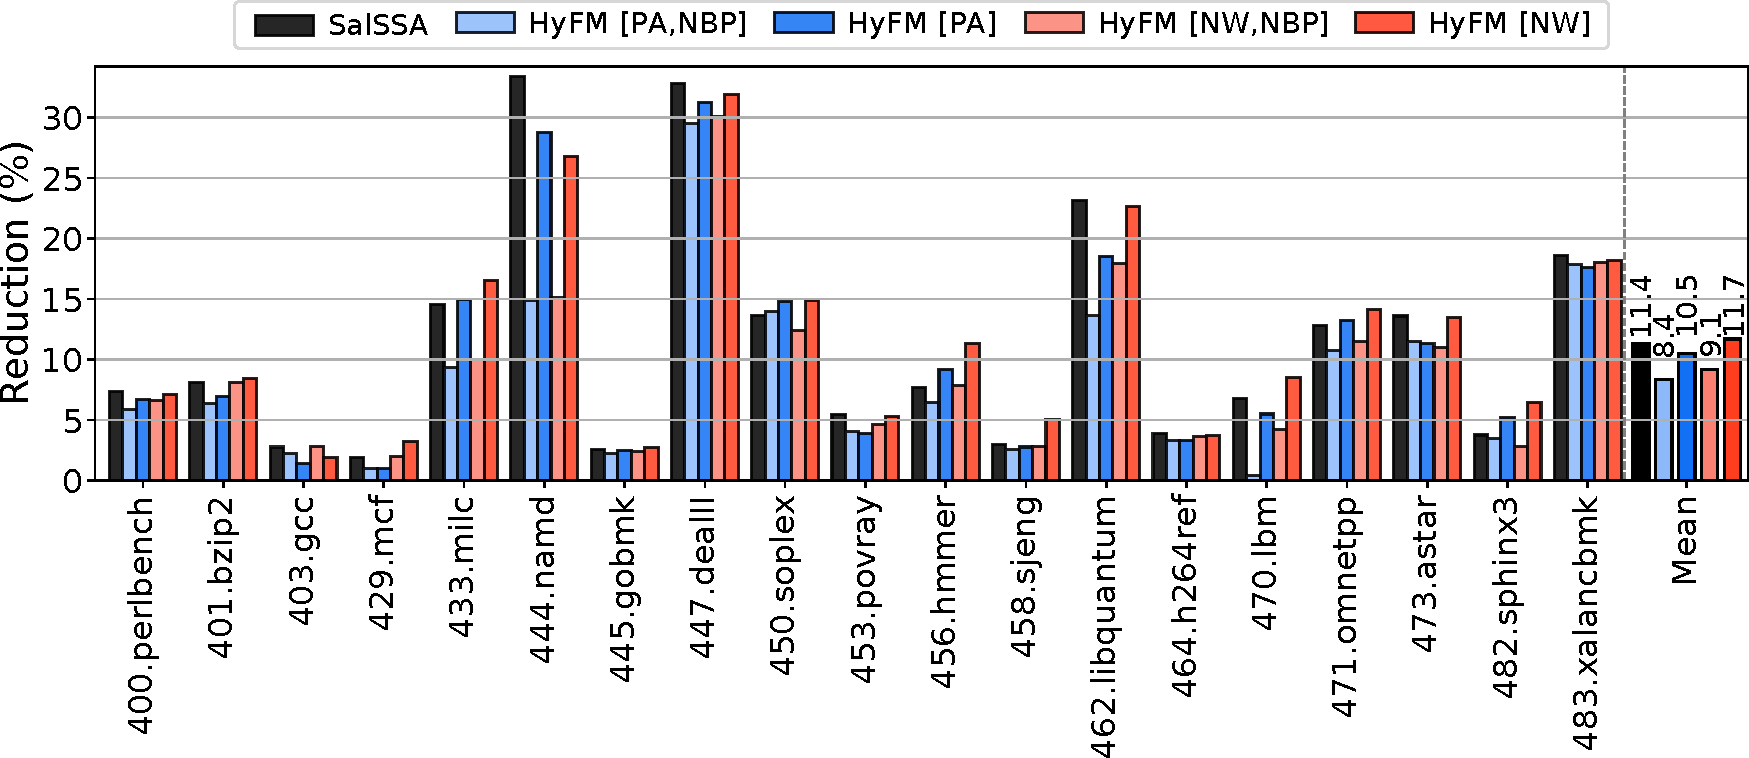
\includegraphics[width=\textwidth]{src/lctes21/figs/reduction-spec06.pdf}
 \caption{SPEC CPU 2006.}
 \label{fig:size-reduction-spec06}
 \end{subfigure}
 \\
 \begin{subfigure}{\textwidth}
 \center
   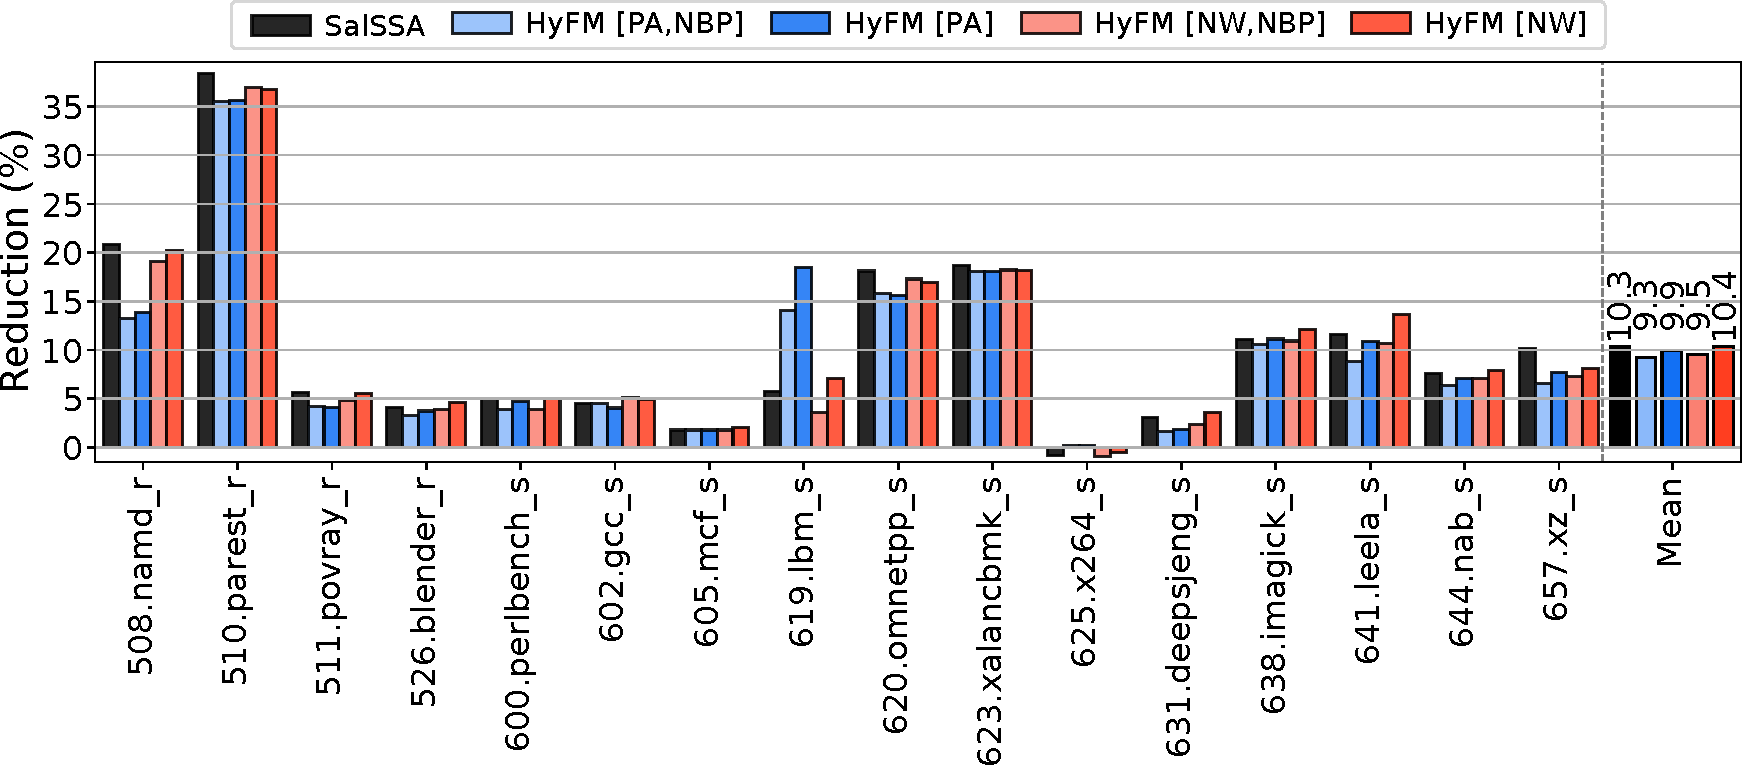
\includegraphics[width=\textwidth]{src/lctes21/figs/reduction-spec17.pdf}
 \caption{SPEC CPU 2017.}
 \label{fig:size-reduction-spec17}
 \end{subfigure}
 \caption{Linked object size reduction over LLVM LTO
      when performing function merging with {\ProjName} or {\SOAName} on SPEC CPU 2006 and 2017. On average, {\ProjName} improves code size reduction.}
  \label{fig:size-reduction-both}
 \end{figure}

%\begin{figure*}[t]
%  \centering
%  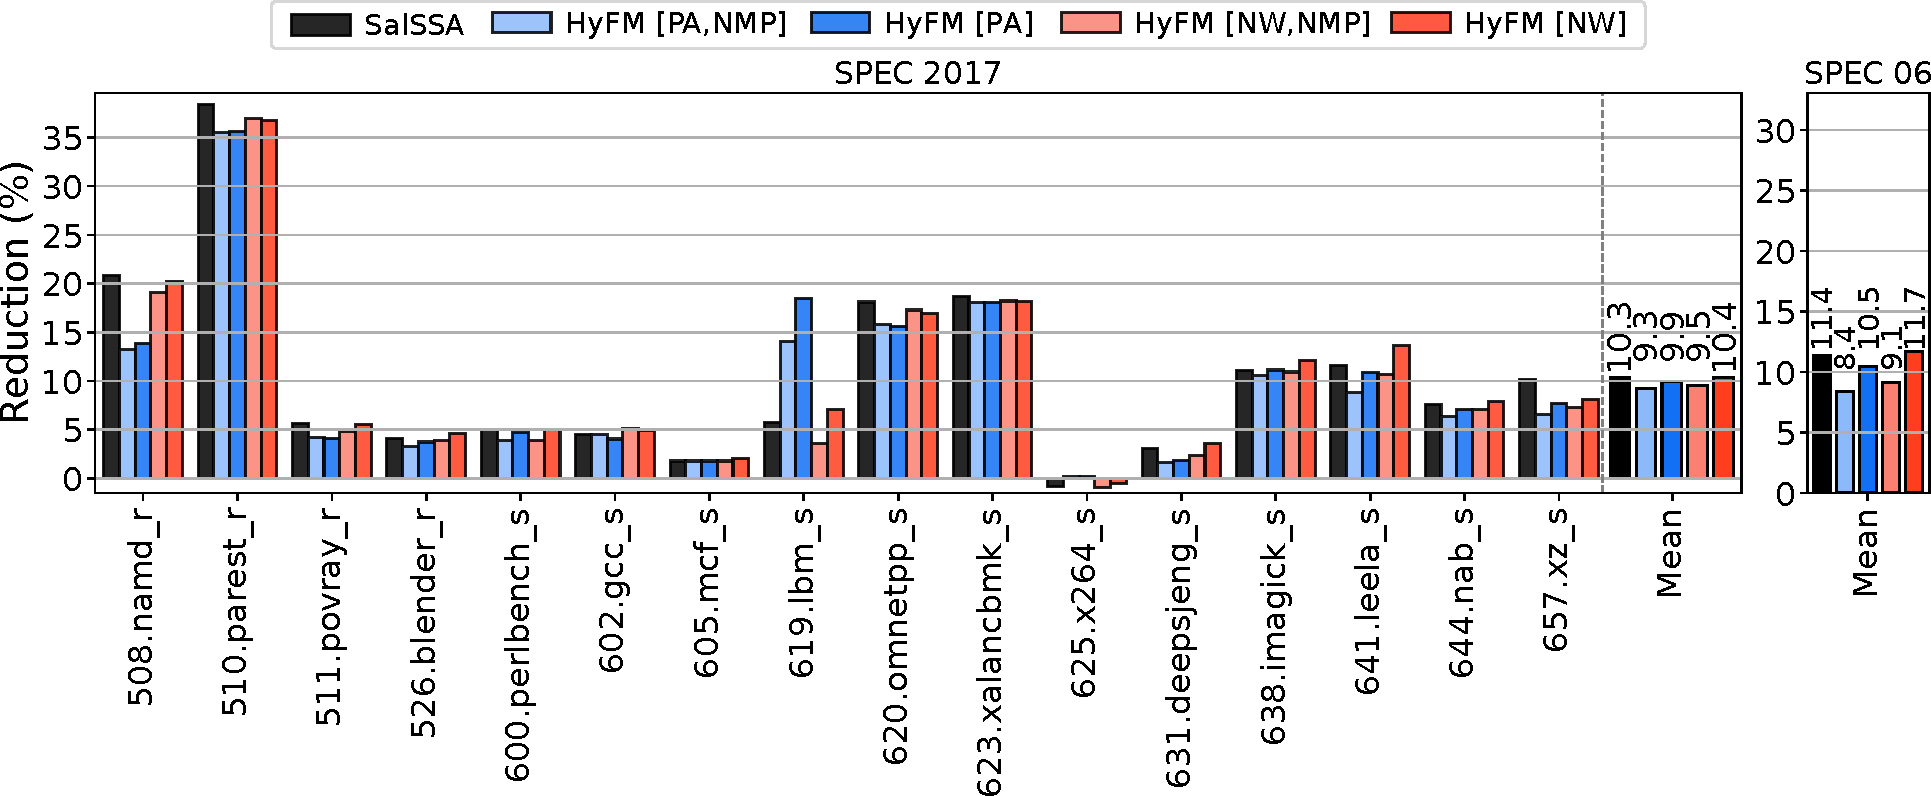
\includegraphics[width=0.95\linewidth]{src/lctes21/figs/reduction-spec17-06.pdf}
%  \caption{Linked object size reduction over LLVM LTO
%      when performing function merging with {\ProjName} or {\SOAName} on SPEC CPU 2006 and 2017. On average, {\ProjName} improves code size reduction.}
%  \label{fig:size-reduction-both}
%\end{figure*}

%Overall, {\ProjName} is on a par with the state of the art {\SOAName}.
%Since our primary aim is to reduce the high compile-time overheads of function merging, as described in Sections~\ref{sec:eval:compilation-time} and \ref{sec:eval:memory}, a small loss of code size reduction is acceptable.

%Even though restricting merging exclusively to basic blocks of the same size seems, at first glance, excessively strong, its effect on code size reduction is limited. On average, same size blocks lead to less than 1\% change compared to the state of the art.

These results indicate that the multi-tier profitability analysis is the single most important component of our approach. 
The two variants without the multi-tier profitability analysis, [PA,NMP] and [NW,NMP], are consistently worse than their counterparts that include this analysis, i.e. [PA] and [NW]. The multi-tier analysis contributes on average about 1 percentage point in code reduction for SPEC 2017 and more than 2 points for SPEC 2006.
The multi-tier profitability analysis has an important impact in the quality of the merged function.
While {\SOAName} lets unprofitable merged subsequences through as long as they are outweighed by profitable subsequences elsewhere in the merged function, {\ProjName} filters such unprofitable subsequences out.

The next most important effect comes from the choice of alignment algorithm. {\NW} is on average half a percentage point better than Pairwise Alignment for SPEC 2017 and about one percentage point better for SPEC 2006. Given that Pairwise Alignment only aligns blocks of the same size and does not try to discover optimal alignments, this difference is smaller than one would expect.
It indicates that profitable pairs of basic blocks tend to be extremely similar if not identical, as discussed in Section~\ref{sec:motivation}.
Still, {\NW} results in more size reduction.
When code size reduction is paramount, [NW] might be a better choice than [PA], but as we will see in Sections~\ref{sec:eval:compilation-time} and \ref{sec:eval:memory}, there is still a trade-off to navigate.

We get the biggest improvement by {[PA]} compared to {\SOAName} and {[NW]} for \texttt{lbm}, where it reduces the program's object file by 18.5\%, almost 13 percentage points more than the competition.
%%%%%%It's actually merging a few profitable basic blocks while giving up on several unprofitable merge sequences
%This comes from discovering a merging opportunity between two large basic blocks of the same size.
%Both {[PA]} and {[PA,NMP]} try merging these blocks but {\SOAName}, {[NW]}, and {[NW,NMP]} choose to focus on other candidates. Compared to {[PA,NMP]}, {[PA]} also finds and profitably merges the same function as {\SOAName} leading to even higher code size reduction.
{\SOAName} is able to profitably merge two pairs of functions.
On the other hand, {[PA,NMP]} chooses to perform a chained merge of the three largest functions in \texttt{lbm}, resulting in a significantly smaller binary.
This is possible because {[PA,NMP]} is merging some nearly identical pairs of basic blocks of the same size.
With the multi-tier profitability analysis, {[PA]} successfully identifies all four cases. 
{[NW]} fails to identify all of these cases, even though it is still better than {\SOAName}.
This exposes existing limitations in the cost model used by our profitability analysis.
%\fixme{Is this a cost model problem?}

The two worst results for {[PA]} are for the \texttt{namd} benchmark in both SPEC 2006 and SPEC 2017. {\SOAName} achieves close to 7 percentage points more than {[PA]} in code size reduction.
In both cases, Pairwise Alignment limits the number of successful merge operations. The variants using {\NW} recover most of the lost reduction. 

% \begin{figure}[h]
%   \centering
%   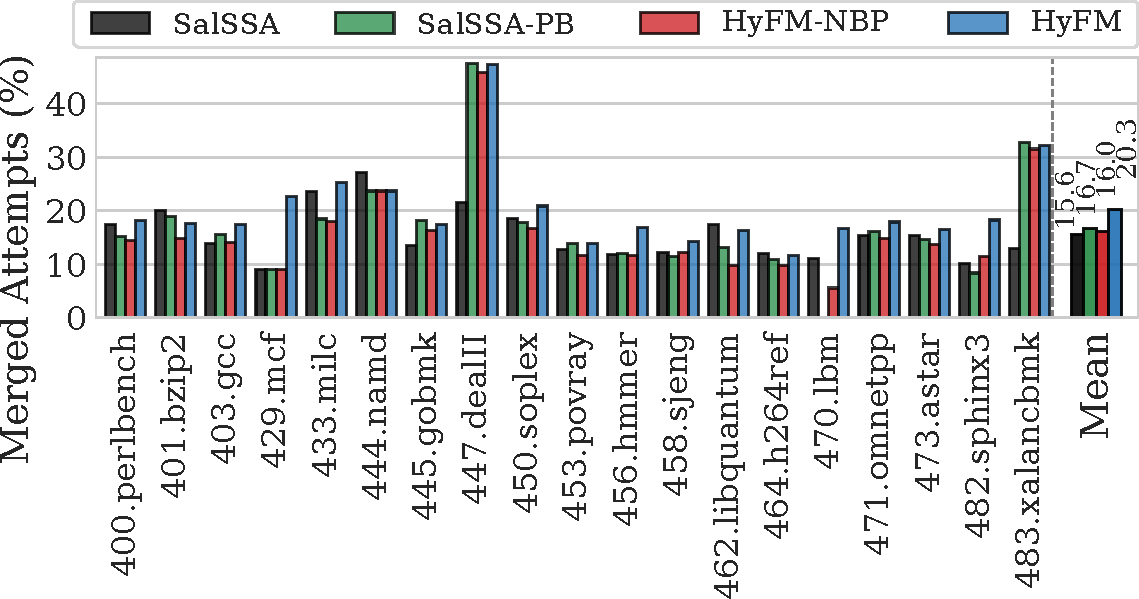
\includegraphics[width=\linewidth]{figs/merged-attempts-perc-spec06.pdf}
%   \caption{Number successful merging attempts on SPEC 2006.}
%   \label{fig:merged-attempts-perc-spec06}
% \end{figure}

% \begin{figure}[h]
%   \centering
%   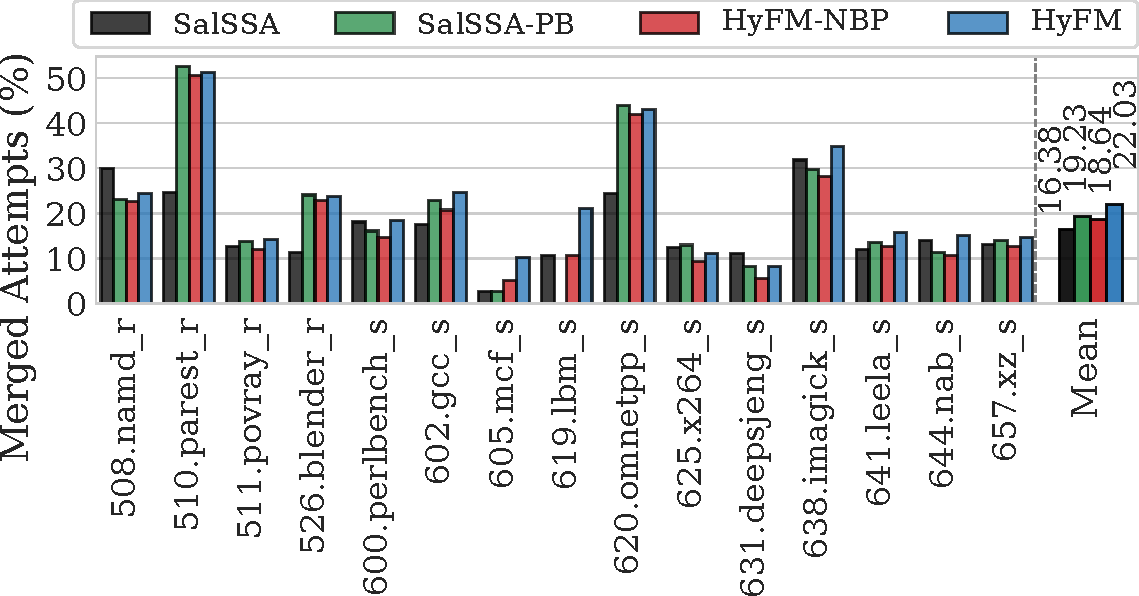
\includegraphics[width=\linewidth]{figs/merged-attempts-perc-spec17.pdf}
%   \caption{Number of successful merging attempts on SPEC 2017.}
%   \label{fig:merged-attempts-perc-spec17}
% \end{figure}

% \begin{figure}[h]
%   \centering
%   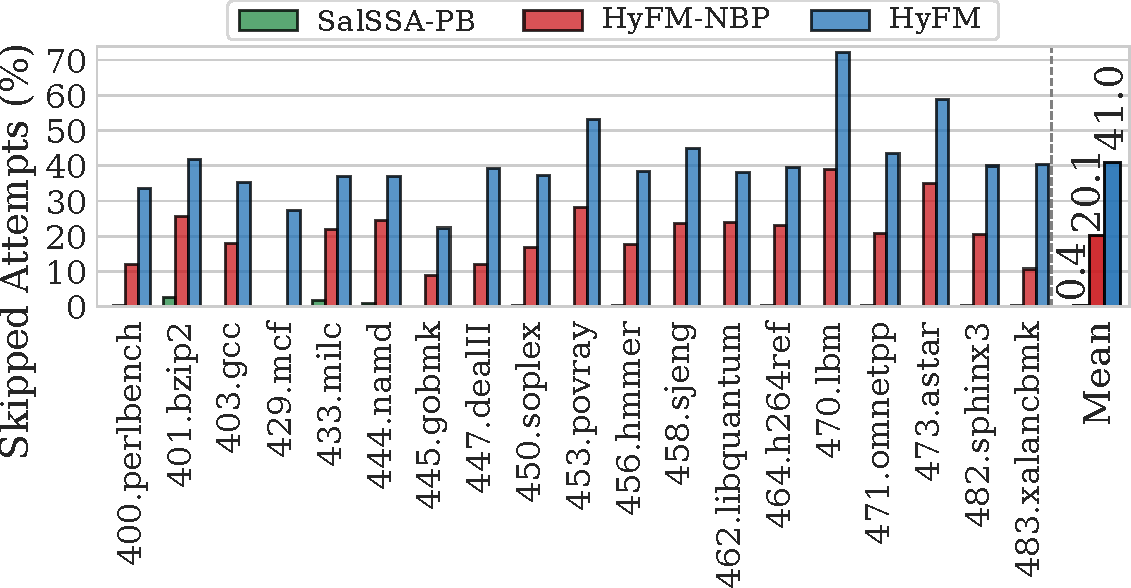
\includegraphics[width=\linewidth]{figs/skipped-attempts-perc-spec06.pdf}
%   \caption{Number of skipped merging attempts on SPEC 2006.}
%   \label{fig:skipped-attempts-perc-spec06}
% \end{figure}

% \begin{figure}[h]
%   \centering
%   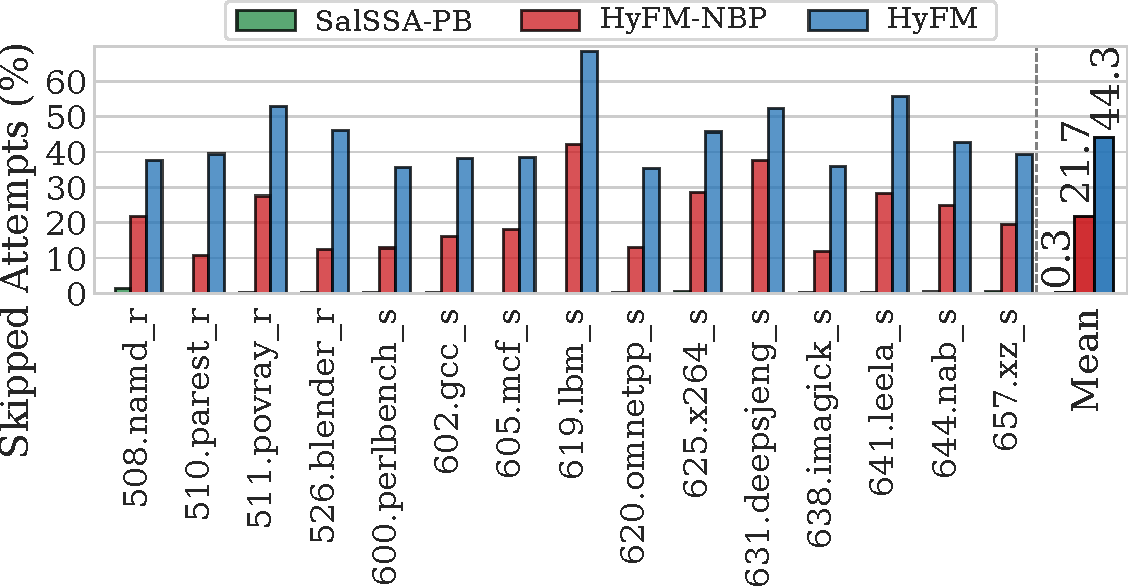
\includegraphics[width=\linewidth]{figs/skipped-attempts-perc-spec17.pdf}
%   \caption{Number of skipped merging attempts on SPEC 2017.}
%   \label{fig:skipped-attempts-perc-spec17}
% \end{figure}


% \begin{figure*}[h]
%   \centering
%   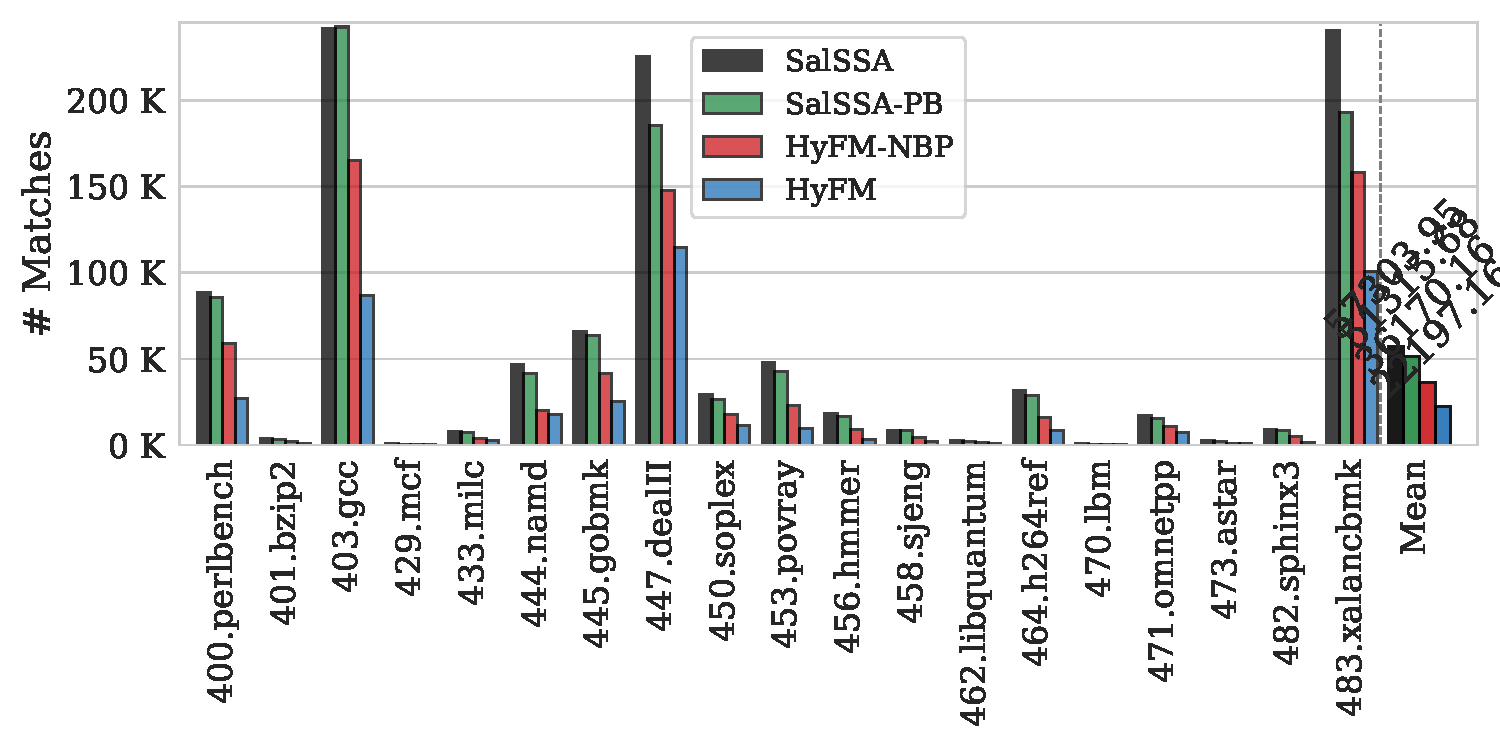
\includegraphics[width=0.85\linewidth]{figs/total-num-matches-spec06.pdf}
%   \caption{Total number of matching entries, including profitable and unprofitable attempts. SPEC 2006.}
%   \label{fig:total-num-matches-spec06}
% \end{figure*}

% \begin{figure*}[h]
%   \centering
%   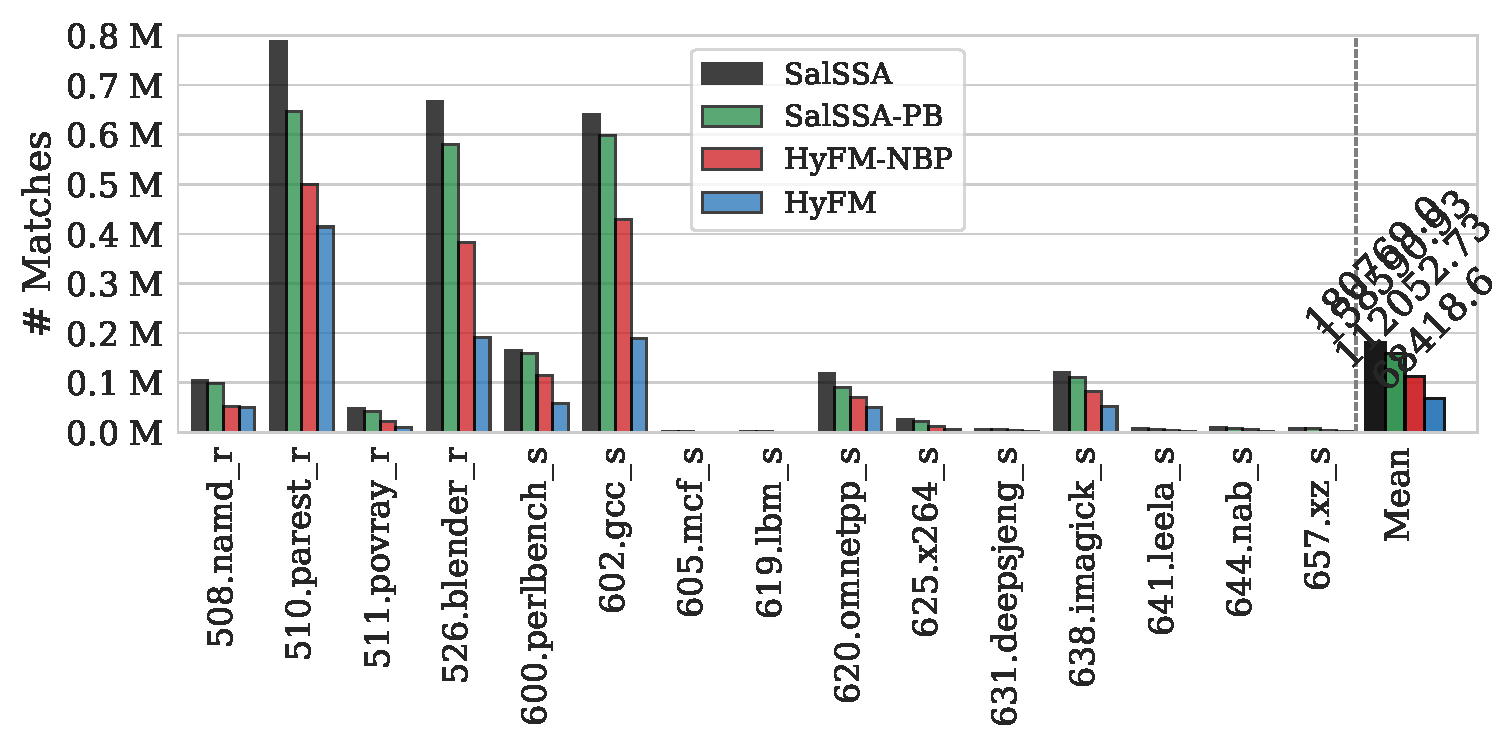
\includegraphics[width=0.85\linewidth]{figs/total-num-matches-spec17.pdf}
%   \caption{Total number of matching entries, including profitable and unprofitable attempts. SPEC 2017.}
%   \label{fig:total-num-matches-spec17}
% \end{figure*}

\subsection{Speeding Up Function Merging} \label{sec:eval:pass-speedup}

 \begin{figure}[h]
   \centering
 \begin{subfigure}{\textwidth}
 \center
   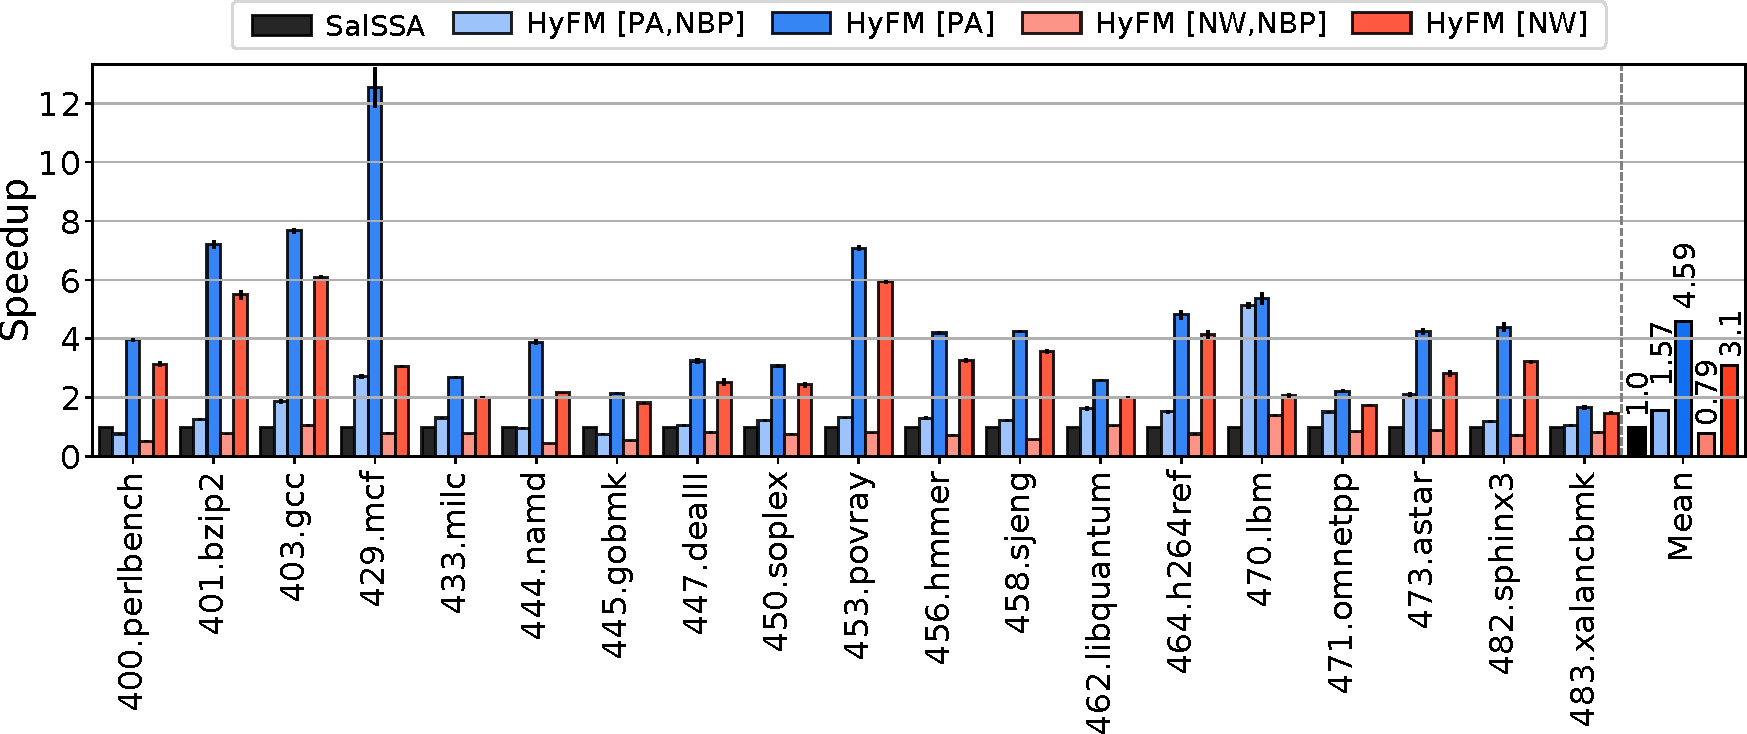
\includegraphics[width=\textwidth]{src/lctes21/figs/speedup-spec06.pdf}
 \caption{SPEC CPU 2006.}
 \label{fig:speedup-spec06}
 \end{subfigure}
 \\
 \begin{subfigure}{\textwidth}
 \center
   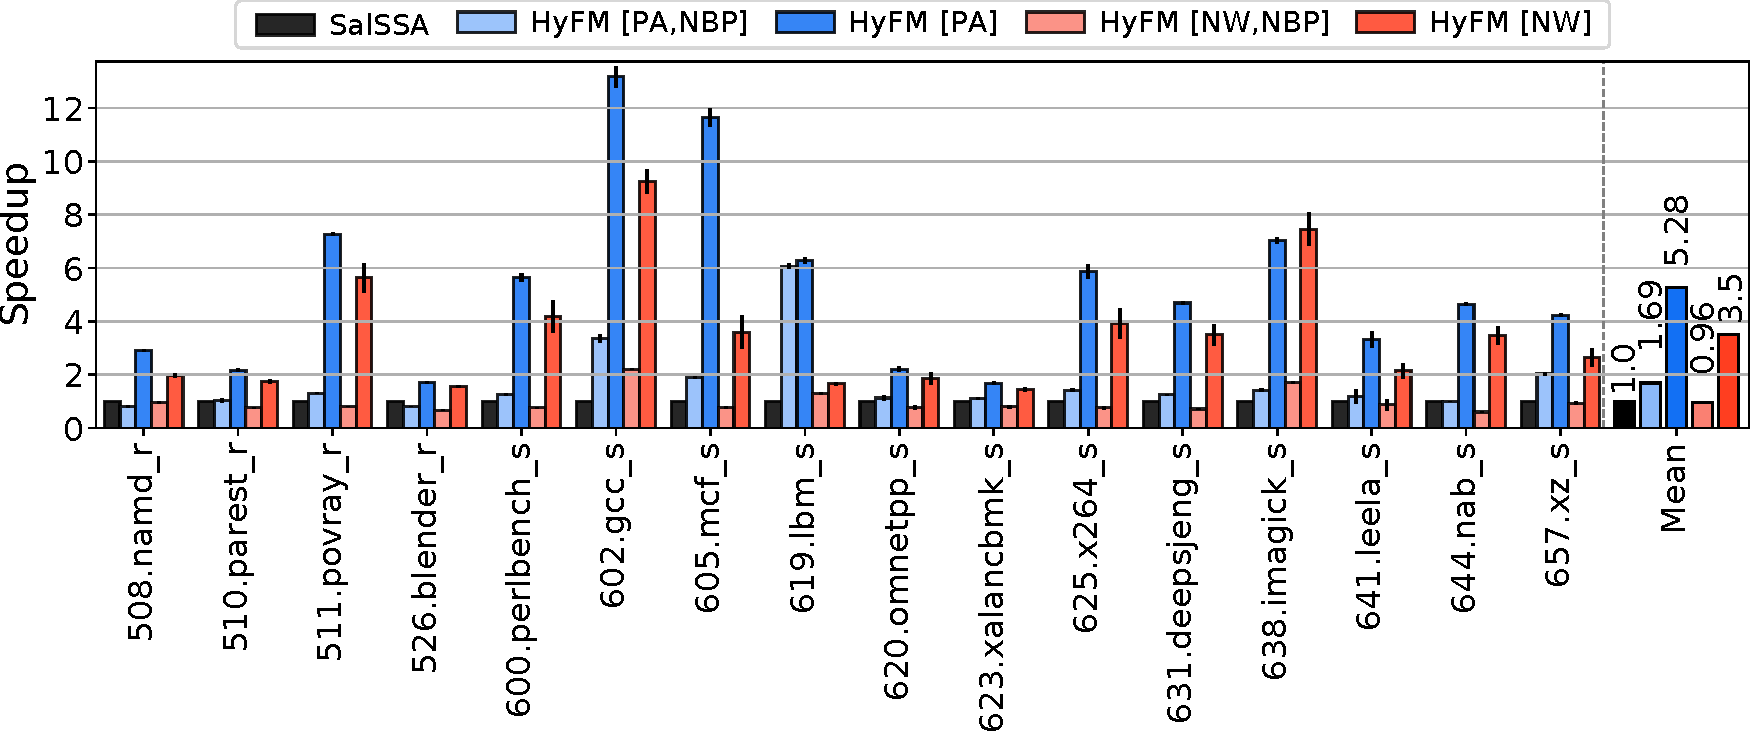
\includegraphics[width=\textwidth]{src/lctes21/figs/speedup-spec17.pdf}
 \caption{SPEC CPU 2017.}
 \label{fig:speedup-spec17}
 \end{subfigure}
 \caption{Speedup of the function merging pass in isolation relative to {\SOAName}. The multi-tier profitability analysis reduces the number of unprofitable merge operations leading to a significant speedup.}
  \label{fig:speedup-both}
 \end{figure}

%\begin{figure*}[t]
%  \centering
%  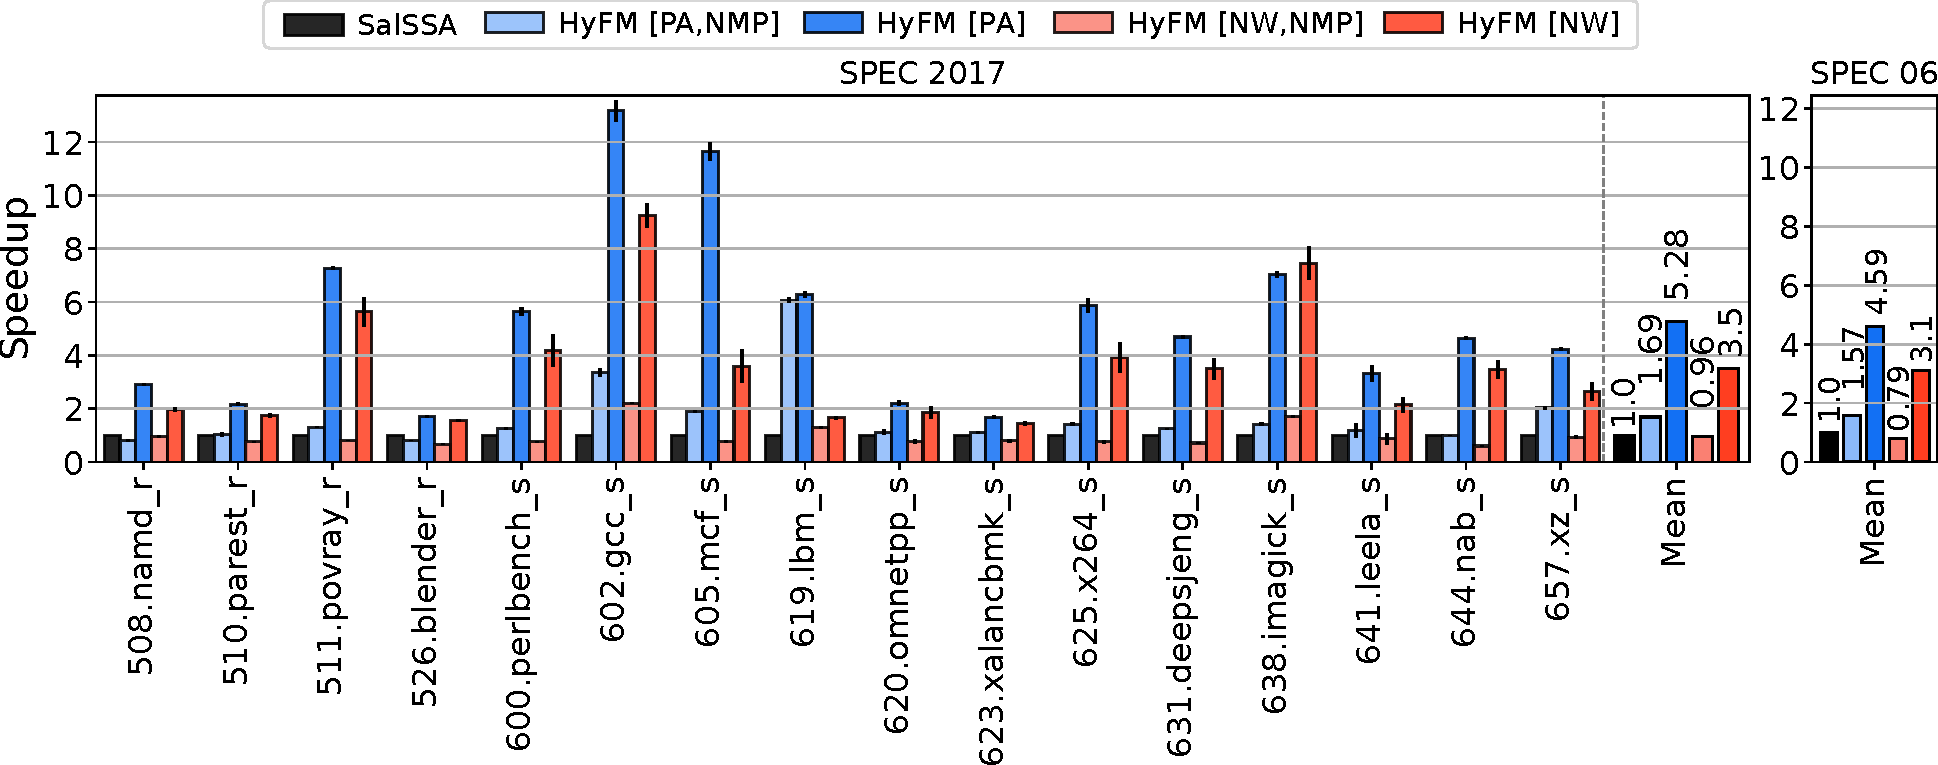
\includegraphics[width=0.95\linewidth]{src/lctes21/figs/speedup-spec17-06.pdf}
%  \caption{Speedup of the function merging pass in isolation relative to {\SOAName}. The multi-tier profitability analysis reduces the number of unprofitable merge operations leading to a significant speedup.}
%  \label{fig:speedup-both}
%\end{figure*}

Figure~\ref{fig:speedup-both} shows the speedup of {\ProjName} relative to {\SOAName}.
This considers only the time taken by the function merging pass, which include all stages discussed in Section~\ref{sec:motivation:breakdown}.
Our novel technique achieves an impressive speedup. For {[PA]} it is on average $5.28\times$ faster for SPEC 2017 and $4.59\times$ for SPEC 2006. Even in the worst case, it achieves a \fixme{50}\% speedup. In the best case, for the SPEC 2017 \texttt{gcc}, function merging under {\ProjName} takes a total of 23.5 seconds instead of 302, which translates to almost $13\times$ less time.

%The two variants with the multi-tier profitability analysis achieve on average three to four times higher speedups than their counterparts without it. This is a direct result of bailing out early. For most benchmarks, only a small number of candidate pairs is profitable. The majority are unprofitable but SalSSA has to merge them anyway to determine their profitability. This is expensive and wasteful. Our approach,on the other hand, is able to estimate profitability early. Only function pairs with any chance of being profitable, that is pairs with at least one profitable pair of basic blocks, move forward to the expensive merge stage.
%The linear pairwise alignment contributes to the performance improvement, too. The variants using pairwise alignment run on average 48% to 98% faster than their Needleman-Wunsch counterparts. The most pronounced case is for lbm where [PA] is around3×faster than [NW]. The blocks paired in lbm are longer than usual, so the quadratic Needleman-Wunsch spends significantly more time trying to align them than our linear pairwise algorithm. Figure 7 shows that the added pairing restrictions from [PA], to focus on blocks with higher similarities, also benefits later stages.
%All components of HyFM contribute towards this result but the multi-tier profitability analysis has the most significant impact. As we show in Figure 7, even though the time spent on the alignment strategy becomes negligible for both [PA,NMP] and [PA], the lack of a multi-tier profitability analysis may degrade the stages associated with code generation. If we accept the alignment for any pair of basic blocks, we may end up producing complex merged functions— code with an excessive amount of branches, phi-nodes,and operand selections — slowing down SSA reconstruction and code simplification. This effect can be observed with [PA,NMP] for many benchmarks in Figure 7. Most notably, for the blender benchmark, [PA,NMP] is slower than SalSSA due to its added pressure on the SSA reconstruction algorithm, even though its alignment strategy runs much faster. For this reason, enabling the multi-tier profitability analysis has a positive impact on later stages.

All components of {\ProjName} contribute towards this result but the multi-tier profitability analysis has the most significant impact. The two variants with the multi-tier profitability analysis achieve on average three to four times higher speedups than their counterparts without it.
To help us understand why, Figure~\ref{fig:breakdown-spec17} shows how the compilation time of each approach is distributed across its various stages. 
Even though the time spent on the alignment strategy becomes negligible with {\ProjName}, the less optimal alignment often produces complex merged functions --- code with an excessive amount of branches, phi-nodes, and operand selections --- slowing down SSA reconstruction and code simplification. This effect is very pronounced for the \texttt{blender} benchmark, where both [PA,NMP] and [NW,NMP] are slower than {\SOAName} due to the added pressure on the SSA reconstruction algorithm, even though the alignment overhead is practically zero.
Similar effects can be observed in other benchmarks.

\begin{figure}[h]
  \centering
  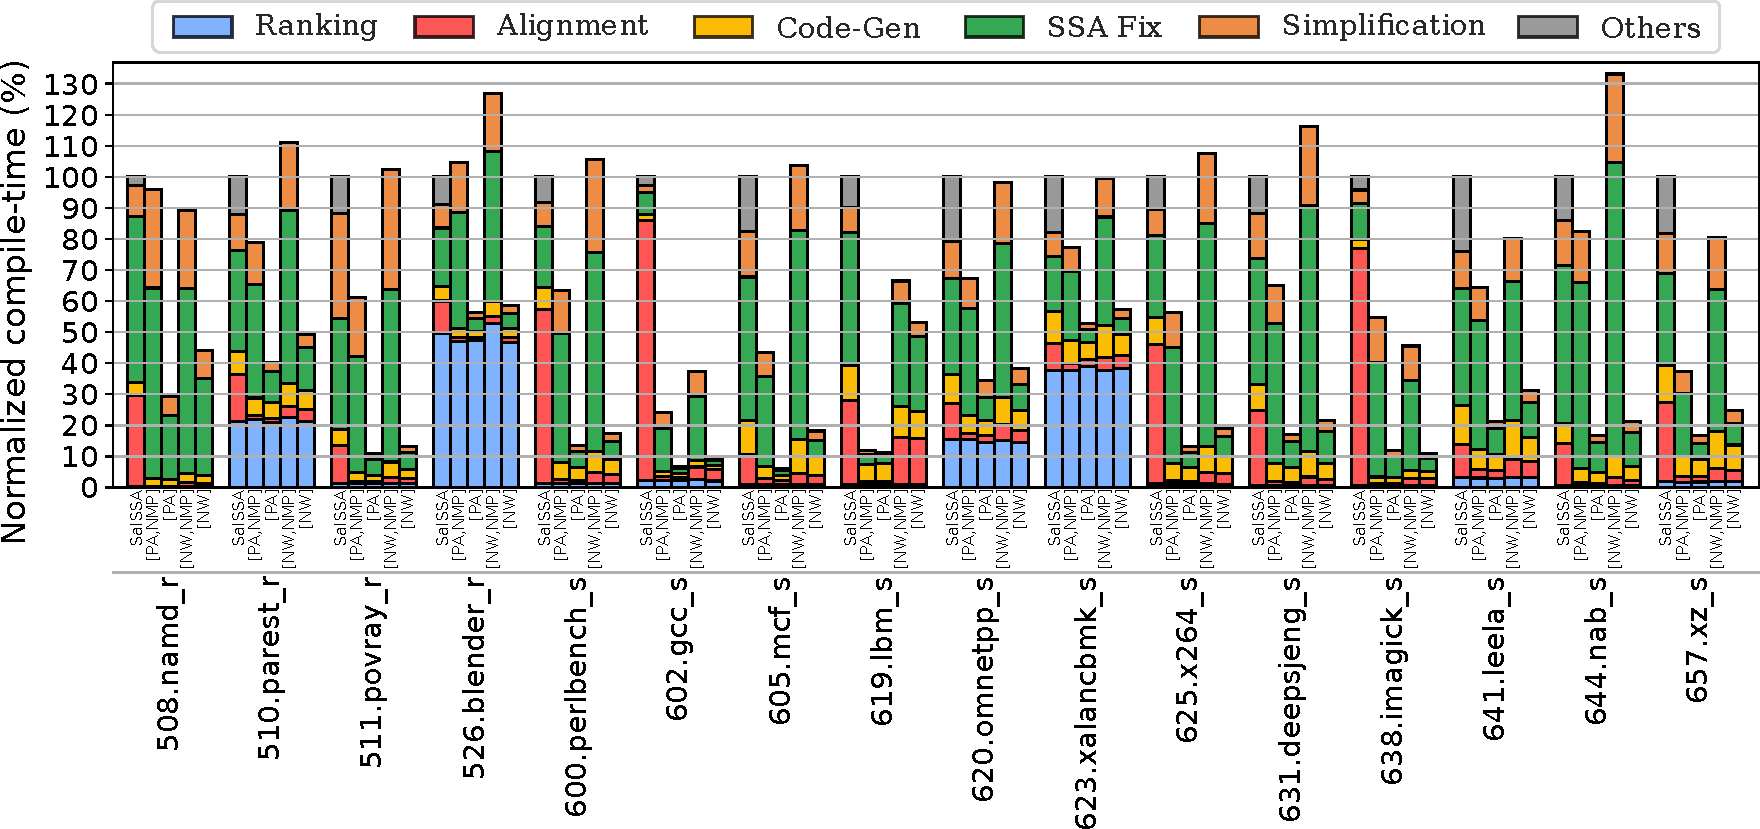
\includegraphics[width=\linewidth]{src/lctes21/figs/breakdown-full-spec17.pdf}
  \caption{Breakdown of the relative runtime for the different stages of the function merging pass. All measurements are normlized by \SOAName's total runtime on the corresponding benchmark. For every benchmark, we show {\SOAName}, [PA,NMP], [PA], [NW,NMP], and [NW], in this order. }
  \label{fig:breakdown-spec17}
\end{figure}

Enabling the multi-tier profitability analysis counters this effect by focusing code generation exclusively on profitable blocks and functions. Most of the complex basic blocks {\ProjName} generates are not profitable for the same reason it is expensive to process them. First-tier profitability filters them out. On top of that, most paired functions under either {\SOAName} or {\ProjName} are unprofitable. {\SOAName} has to merge them anyway to determine their profitability. This is expensive and wasteful. Our approach, on the other hand, is able to estimate profitability early. Only function pairs with any chance of being profitable, that is pairs with at least one profitable pair of basic blocks, move forward to the expensive merge stage.

The linear pairwise alignment contributes to the performance improvement, too. The variants using pairwise alignment run on average 48\% to 98\% faster than their {\NW} counterparts.
%The most pronounced case is for \texttt{mcf} where {[PA]} is approximately $3\times$ faster than {[NW]}. Candidate basic block pairs in \texttt{mcf} are longer than usual, so the quadratic {\NW} spends significantly more time trying to align them than our linear pairwise algorithm. 
The most pronounced case is for \texttt{lbm} where {[PA]} is around $3\times$ faster than {[NW]}. The blocks paired in \texttt{lbm} are longer than usual, so the quadratic {\NW} spends significantly more time trying to align them than our linear pairwise algorithm.
Figure~\ref{fig:breakdown-spec17} shows that the added pairing restrictions from [PA], to focus on blocks with higher similarities, also benefits later stages.

\subsection{End-to-End Compilation Time} \label{sec:eval:compilation-time}

We have also analyzed separately the end-to-end compilation time because reducing code size through function merging has knock-on effects in later stages of the compilation pipeline.
The first order effect is that reducing the number of functions tends to reduce compilation time.
This is not guaranteed though, because merged functions may be more complex, potentially slowing down later compiler analyses and transformations.
Moreover, the time spent merging functions may be so large that it negates any benefits from having fewer functions later in the pipeline.

Even though on a few occasions {\SOAName} reduces end-to-end compilation time, in general, its overhead is large enough to result in an overall compilation time slowdown, 9.5\% to 4.1\% for SPEC 2017 and 2006 respectively.
In contrast, {\ProjName} is so much faster that its compilation time overhead is matched or outweighed by the speedup in later stages. 
This reduction is marginal for SPEC 2017, but for SPEC 2006 {[PA]} reduces the average compilation time by 2.3\% and {[NW]} by 1.6\%.
There is only a single case where {[PA]} results in a significant end-to-end slowdown, 10\% for \texttt{blender}.
%While this is still an improvement compared to {\SOAName}, \fixme{EXPLAIN}.
Figure~\ref{fig:breakdown-spec17} shows that, although [PA] runs faster than {\SOAName}, both of them spent a significant amount of time ranking the function candidates, due to its large number of functions.
Ranking alone in this case takes around 70 seconds. %However, this is beyond the scope of this paper.

Overall, we believe that this reduction in end-to-end compilation time is a very important result. While {\ProjName} is still achieving code-size reduction on par with the state-of-the-art, it does not have the detrimental effects of {\SOAName} on the overall compilation process and can be safely applied.

 \begin{figure}[h]
   \centering
 \begin{subfigure}{\textwidth}
 \center
   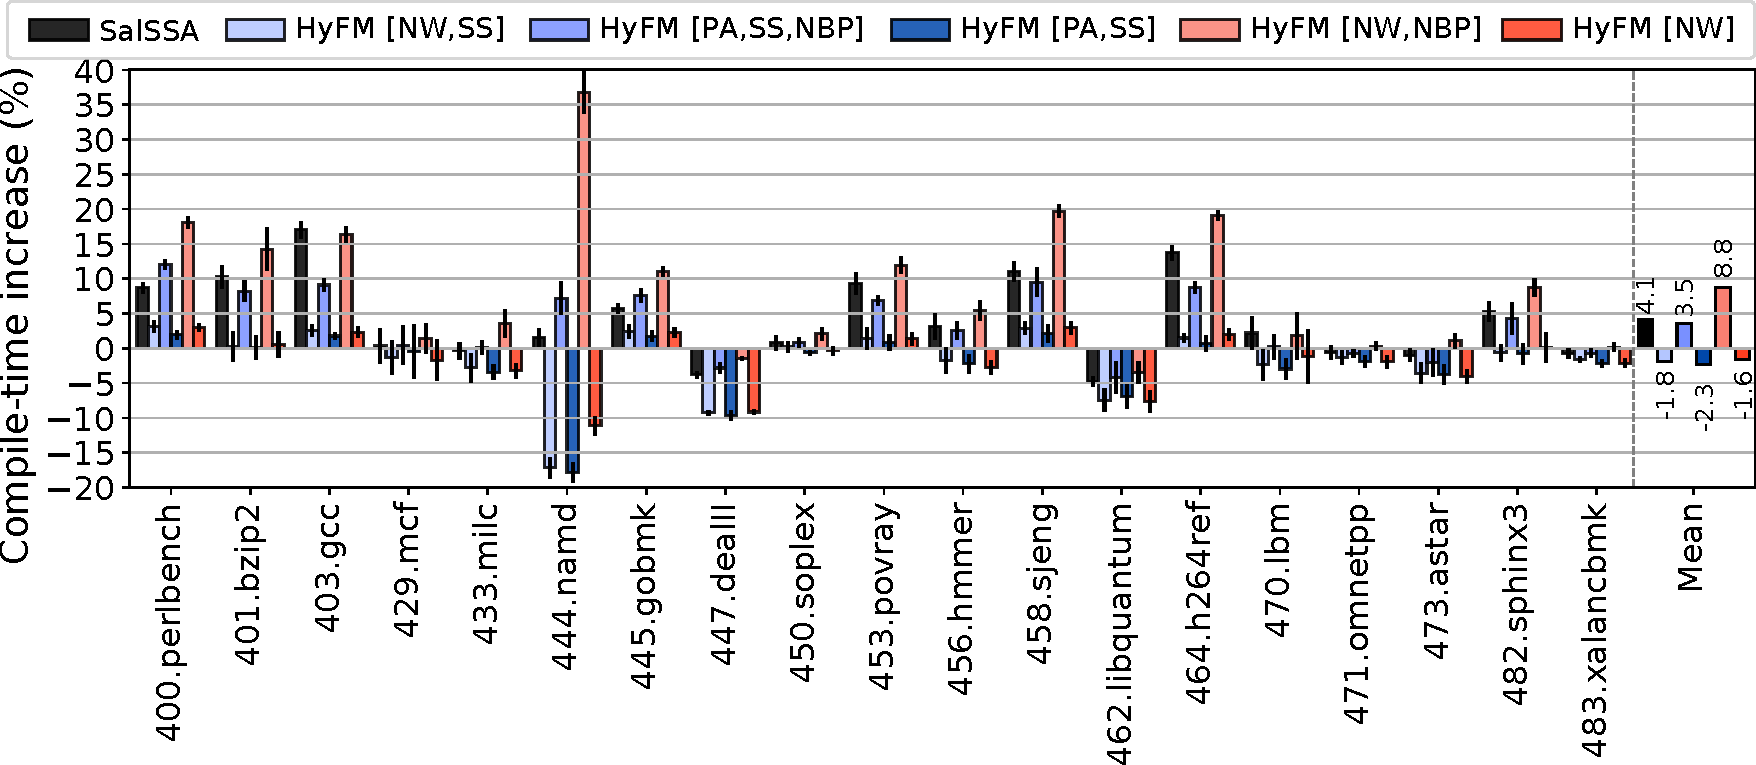
\includegraphics[width=\textwidth]{src/lctes21/figs/compiletime-spec06.pdf}
 \caption{SPEC CPU 2006.}
 \label{fig:compiletime-spec06}
 \end{subfigure}
 \\
 \begin{subfigure}{\textwidth}
 \center
   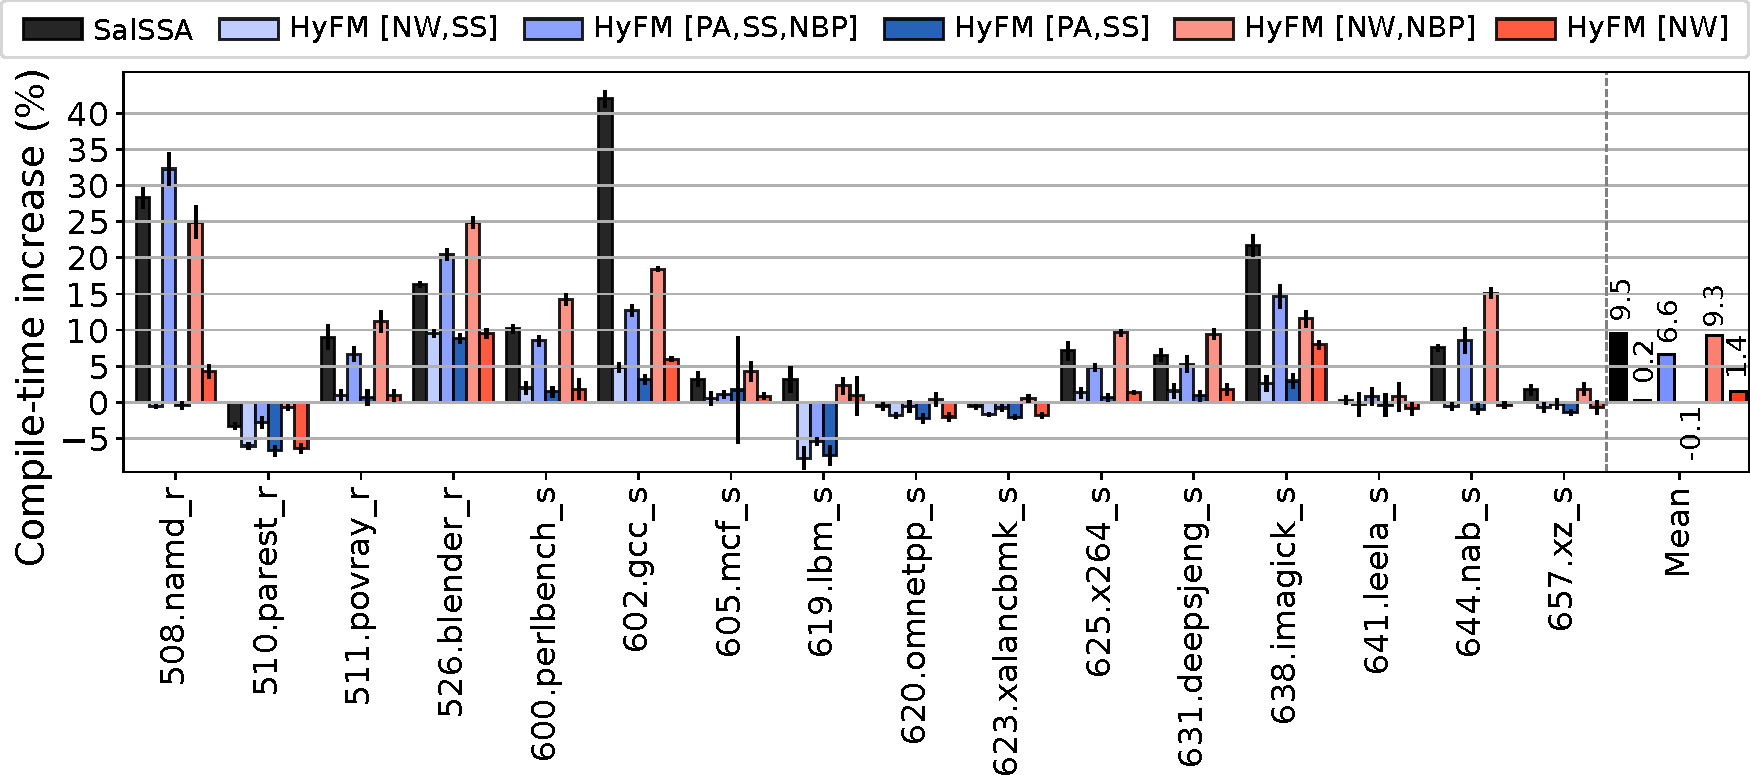
\includegraphics[width=\textwidth]{src/lctes21/figs/compiletime-spec17.pdf}
 \caption{SPEC CPU 2017.}
 \label{fig:compiletime-spec17}
 \end{subfigure}
 \caption{Normalized end-to-end compilation time for SPEC 2017 and SPEC 2006 relative to LLVM LTO.}
  \label{fig:compiletime-both}
 \end{figure}

%\begin{figure*}[h]
%  \centering
%  \includegraphics[width=0.95\linewidth]{src/lctes21/figs/compiletime-spec17-06.pdf}
%  \caption{Normalized end-to-end compilation time for SPEC 2017 and SPEC 2006 relative to LLVM LTO.}
%  \label{fig:compilation-both}
%\end{figure*}


\subsection{Code Size and Compilation Time Trade-Off} \label{sec:eval:trade-off}

While the multi-tier profitability analysis improves both code-size reduction and compilation speed, the choice of alignment algorithm introduces a trade-off. Pairwise alignment is better for speed, {\NW} is better for code-size reduction. 
In terms of compilation efficiency, i.e. how much code size reduction we get for the effort we put in, the picture is clearer. In Figure~\ref{fig:ars-both}, the \textit{average reduction speed} suggests that {[PA]} achieves the ideal trade-off, with an average reduction speed of 115.3~KB/s, which is around $3\times$ greater than {\SOAName}'s and 20\% to 40\% greater than [NW].


 \begin{figure}[h]
   \centering
 \begin{subfigure}{\textwidth}
 \center
   \includegraphics[width=\textwidth]{src/lctes21/figs/ars-spec06.pdf}
 \caption{SPEC CPU 2006.}
 \label{fig:ars-spec06}
 \end{subfigure}
 \\
 \begin{subfigure}{\textwidth}
 \center
   \includegraphics[width=\textwidth]{src/lctes21/figs/ars-spec17.pdf}
 \caption{SPEC CPU 2017.}
 \label{fig:ars-spec17}
 \end{subfigure}
 \caption{Average reduction speed on both SPEC 2006 and 2017.}
  \label{fig:ars-both}
 \end{figure}

%\begin{figure*}[h]
%  \centering
%  \includegraphics[width=0.95\linewidth]{src/lctes21/figs/ars-spec17-06.pdf}
%  \caption{Average reduction speed on both SPEC 2006 and 2017.}
%  \label{fig:ars-both}
%\end{figure*}

\subsection{Memory Usage} \label{sec:eval:memory}

 \begin{figure}[h]
   \centering
 \begin{subfigure}{\textwidth}
 \center
   \includegraphics[width=\textwidth]{src/lctes21/figs/memory-spec06.pdf}
 \caption{SPEC CPU 2006.}
 \label{fig:memory-spec06}
 \end{subfigure}
 \\
 \begin{subfigure}{\textwidth}
 \center
   \includegraphics[width=\textwidth]{src/lctes21/figs/memory-spec17.pdf}
 \caption{SPEC CPU 2017.}
 \label{fig:memory-spec17}
 \end{subfigure}
 \caption{Peak memory usage of {\SOAName} and {\ProjName} variants for SPEC 2006 and 2017 in log scale. {\SOAName} has a peak memory usage several orders of magnitude hundreds higher than all other approaches. The pairwise alignment variants of {\ProjName} need on average only a seventh of the memory needed by the {\NW} variants.}
  \label{fig:memory-both}
 \end{figure}

%\begin{figure}[h]
%  \centering
%  \includegraphics[width=\linewidth]{src/lctes21/figs/memory-spec17-06-tiny.pdf}
%  \caption{Peak memory usage of {\SOAName} and {\ProjName} variants for SPEC 2006 and 2017 in log scale. {\SOAName} has a peak memory usage several orders of magnitude hundreds higher than all other approaches. The pairwise alignment variants of {\ProjName} need on average only a seventh of the memory needed by the {\NW} variants.}
%  \label{fig:memory-both}
%\end{figure}

Another important aspect of function merging is peak memory usage. This is especially critical for an optimization designed for LTO.
Compilation in full LTO mode is already memory hungry. Just keeping the whole program in memory can be a significant problem for large programs~\cite{johnson17}. Maintaining additional information for every function and basic block could easily tip the compiler over the edge.

Figure~\ref{fig:memory-both} shows the peak memory usage (in log scale) needed for the alignment stage alone.
For {\SOAName}, this represents simply the execution of the {\NW} algorithm.
For {\ProjName}, the alignment stage represents both aligning each pair of basic blocks as well as the pairing these basic blocks.
Our results show that {[PA]} is over three orders of magnitude better than {\SOAName}, while {[NW]} is more than two orders of magnitude better.
In other words, while {\SOAName} requires on average 2.4~GB of memory, {[PA]} uses only around 610~KB and {[NW]} uses 5.6~MB.

The peak memory usage is especially noticeable on \texttt{gcc}, when merging its two largest functions, containing 90093 and 76265 instructions.
Since {\SOAName} applies its quadratic sequence alignment algorithm on the linearized sequences of the whole input functions, it uses over 32~GB of memory when merging these two functions.
Meanwhile, {[NW]} requires only around 5.6~MB for merging the same pair of input functions, even though it employs the same sequence alignment algorithm. This is because its peak memory usage is a quadratic function of the largest pair of \emph{blocks} instead of the largest pair of \emph{functions}.
Although very large, these two functions are composed of several thousands of very small basic blocks, so the memory overhead of {\NW} is limited.
Most of the memory consumed by {[NW]} in this case is actually needed for storing the basic block fingerprints.
This aspect becomes evident when we compare the peak memory usage of {[NW]} with that of the {[PA]} for \texttt{gcc}. They have similarly low memory requirements, even though only one of them uses a quadratic alignment algorithm.

In other cases, where basic blocks are longer, pairwise alignment leads to a significantly lower peak memory usage compared to {\NW}. For \texttt{parest}, for example, pairwise alignment reduces memory usage from \fixme{40}~MB to \fixme{200}~KB. Overall, {[PA]} needs around $6\times$ less memory. For smaller programs, {[NW]} might be a viable option but for larger ones being able to reduce memory usage to a minimum might be more important.

% \subsection{Summary}
% Overall, our novel function merging technique has surpassed the state-of-the-art in terms of compilation time, memory usage, as well as code size reduction.
% However, different variants of the proposed technique are better suited for different goals.
% If the code size is the utmost concern, {\ProjName}~[NW] is the winning strategy, but if we are looking for the most balanced trade-off between compilation-time overheads and code-size reduction, {\ProjName}~[PA] has shown better results.


\chapter{Conclusion} \label{chp:conclusion}

This thesis presents a novel compiler optimisation for reducing code size by merging functions.
Chapter~\ref{chp:fm-operation} describes our novel approach, based on sequence alignment, for merging any two functions.
Chapter~\ref{chp:opt-strategy} describes how our function merging technique can be combined with a optimisation strategy in order to search for profitable functions to merge, which includes a profitability cost model and a ranking of candidate functions.

This chapter is structured as follows:
Section~\ref{sec:conclusion:contribution} summarises the main contributions of this thesis,
%Section 7.2 presents a critical analysis of this work,
Section~\ref{sec:conclusion:futurework} describes future research directions,
and finally Section~\ref{sec:conclusion:summary}  provides concluding remarks.


% We have presented {\ProjName}, a novel compiler-based function merging technique with full support for the SSA form.
% Unlike the previous state-of-the-art, which has to apply register demotion to eliminate the commonly used \textit{phi-nodes} in SSA,
% {\ProjName} directly processes \textit{phi-nodes} using a more powerful code generator.
% As a result, {\ProjName} avoids the code bloating problem introduced by register demotion and
% increases the chances of generating profitable merged functions. We have implemented {\ProjName} in LLVM and evaluated it on the SPEC CPU2006
% and CPU2017 benchmark suites. {\ProjName} delivers on average 9.5\% code reduction for the lowest exploration threshold. Compared to the previous
% function merging state-of-the-art, {\ProjName} achieves $2\times$ more reduction on binary size with 3$\times$ less compile-time overhead and less than half the amount of memory required by it.

% We proposed a novel function merging approach based on sequence alignment, called FMSA. This was the first technique capable of merging any two functions, if deemed profitable, achieving up to 30\% of code-size reduction on SPEC 2006, about twice as much as the past state of the art.
% Although this technique offers significant improvements over previous ones, there are still many limitations and missed opportunities that prevent us from achieving all the available code compression.
% We need to improve the code generator, exploit code reordering, work at different scopes, scale to huge programs, avoid runtime slowdowns, work on JITs, and adopt machine learned heuristics.
% %To address these missed opportunities,
% %We plan to create a better code generator, a new approach that handles code reordering and merges code across different scopes, more accurate cost models
% %, with a better ranking mechanism and code aligner powered by deep learning.
% This will result in smaller programs without runtime or compile time overheads.

\section{Contribution} \label{sec:conclusion:contribution}

This thesis presents a novel function merging technique alongside an optimisation strategy.
Our novel technique uses sequence alignment algorithms from bioinformatics in order to identify the similarity between functions being merged.
The proposed optimisation is very effective at reducing code size by merging arbitrary functions.
Our approach does not suffer from any of the major limitations of existing solutions, outperforming them by more than 2.4$\times$.
We also proposed a ranking-based exploration mechanism to focus the optimization on promising pairs of functions.
Ranking reduces the compilation-time overhead by orders of magnitude compared to an exhaustive quadratic exploration. 
With this framework, our optimization is able to reduce code size by up to 25\%, with an overall average of about 6\%, while introducing an average compilation-time overhead of only 15\%.
Coupled with profiling information, our optimization introduces no statistically significant impact on performance.

\section{Future Work} \label{sec:conclusion:futurework}

For future work, we plan to focus on improving the ranking mechanism to reduce compilation time.
In order to avoid code size degradation, we also plan to improve the compiler's built-in static cost model for code size estimation.
We also plan to work on the linearisation of the candidate functions, allowing instruction reordering to maximize the number of matches between the functions.
Finally, we also plan to incorporate instruction reordering into function merging to maximize the number of matches between the functions regardless of the original code layout.
One can also investigate the application of phi-node coalescing outside function merging.
We envisage further improvements can be achieved by integrating the function-merging optimization to a summary-based  link-time optimization framework, such as ThinLTO in LLVM.
As a future work, we can also analyze the interaction between function merging and other optimizations such as inlining, outlining, and code splitting.

\subsection{Better Code Generator}

%FMSA's code generator is responsible for producing the actual merged functions from the aligned sequences.
%In its original version, FMSA has many artificial limitations in order to simplify its code generator.
%Preliminary results show that the code generator can be significantly improved, enabling far more code compression while reducing compilation time overhead.
%For this project, we plan to develop a new code generator that is capable of appropriately handling $\phi$-nodes, variable length arguments, calling convention, and exploiting target specific instructions to better compress code.
%There are still many opportunities to optimize operand selection and branch instructions that result from merging code. 

In order to better compress code, one can improve the code generator, optimising the parameters used as function identifiers based on calling conventions, exploit target specific instructions, and optimize operand selection and branch instructions that result from merging code.
There are also many missing features in the code generator that are important for its application in the industry.
For example, a new code generator could also be able to appropriately handle variable length arguments, and debug information.
When merging functions, having an optimised code generator is as important as optimally identifying which instructions to merge.
%In the industry, it is also crucial that we appropriately handle debug information when generating code. %link with: \phi$-nodes, variable length arguments
%Appropriately generating code with debug information is crucial for its application in the industry.

\subsection{Handling Code Reordering}

All existing function merging techniques rely on the order in which instructions appear inside the basic blocks and their arrangement,
failing to profitably merge equivalent functions when confronted even with the smallest variations on the ordering of instructions and basic blocks.
Figure~\ref{fig:code-reordering} shows an example of two functions that all existing techniques fail to merge even though they are obviously identical.
Our current technique produces the merged function shown in Figure~\ref{fig:merged-code-reordering}, which is considered unprofitable as it is unable to reduce code size.
Note that all indexing computation is duplicated, including the increment operation, resulting in a merged function that is unnecessarily bigger than the two original functions together.
We need more powerful graph, rather than sequence, alignment techniques to better identify and merge differently ordered but semantically equivalent code.

\begin{figure}[h]
 \centering
 \begin{subfigure}{.5\textwidth}
         \centering
         \includegraphics[scale=0.85]{src/conclusion/figs/motivation-1-code.pdf}
         \vspace{1ex}
         \caption{Two equivalent functions.}
         \label{fig:code-reordering}
 \end{subfigure}\begin{subfigure}{.5\textwidth}
         \centering
         \includegraphics[scale=0.85]{src/conclusion/figs/motivation-1-merged-code.pdf}
         \caption{Merged function currently produced by FMSA.}
         \label{fig:merged-code-reordering}
 \end{subfigure}
    \vspace{-2ex}
    \caption{Example of how even trivial reordering is poorly handled by the existing solutions.}
    \label{fig:code-reordering-example}
\end{figure}

\subsection{Merging Across All Scopes}

Existing techniques are limited to one particular scope.
While function merging is applied only to whole functions,
function outlining is commonly applied at the basic block level.
%In one end we have an optimization such as the function outlining which is capable of merging or extracting equivalent basic blocks, in the other end we have function merging capable of merging whole functions.
However, equivalent code can be found within or across functions, which themselves may reside in the same source file or be spread across multiple source files.
Therefore, we need to develop a novel unified optimization capable of merging semantically equivalent code that can span anything between a single basic block up to a whole function.
This unification has the extra benefit of also addressing the phase ordering problem by coordinating the merge operations on different scopes.

\subsection{Scaling for Large Programs}

Although our optimisation achieves very good results in terms of code compression, it is still unable to handle large programs in a real scenario.
Its time complexity and memory usage requirements would prevent it from optimizing large programs such as web browsers, Clang/LLVM, and operating systems, as these programs tend to have many functions with several thousands of instructions.
Link-time optimization (LTO) makes this matter even worse by optimizing the code after the whole program has been linked into a single module, imposing a huge pressure on memory usage and compilation time.

%In this project, we will investigate this scalability issue.
%We plan to perform link-time optimization in an incremental fashion, such as using ThinLTO, which operates on individual translation units, reducing memory usage while also making it suitable for parallel and distributed compilation.
The optimization of different translation units can be distributed across different machines and merge operations locally performed in parallel.
In order for this to work, an important challenge that needs to be addressed concerns ranking and merging functions that reside in different translation units.
However, this is essential to enable the use of LTO on real programs while keeping the memory usage and compilation time acceptable.

\subsection{Powered by Deep Learning}

In order to reduce compilation time while also being effective, 
the ranking-based exploration mechanism tries to efficiently focus the search 
only to the most promising pairs of functions.
However, the existing solution is still very wasteful as most of the merged functions are
discarded by the profitability analysis.
Identifying what would be profitably merged is a very challenging task.

Given our group's expertise on the area, we plan to use solutions based on deep learning to efficiently predict which pairs of functions are most likely to be profitable to merge.
This approach has the potential to reduce compilation time even further while also improving the compression by finding profitable candidates that are currently missed.
Having accurate target-specific cost models is crucial for the effectiveness of the profitability analysis.
We plan to explore the use of machine learning techniques to develop more accurate cost models.

One can investigate the use of deep learning to align two functions and better identifying what can be merged.
Sequence alignment focusses only on maximizing the number of merged instructions,
without necessarily minimizing the number of operand selections or branches.
A smarter approach that understands how instructions interact with each other would be
very beneficial.


\subsection{Avoiding Performance Overheads}

For many real applications, it is desirable to achieve a good balance between code size and performance.
Preliminary results show that performance degradation can be completely avoided by using profiling to
guide the merging decisions.
One can avoid adding branches inside hot execution paths, therefore avoiding performance penalties.
Although hot code can be merged, it is important to minimize unnecessary branches when merging hot code.
We will develop a profile-guided optimization that automatically identify the best trade-off between code-size and performance.

\subsection{Less Memory Usage by JIT}

Ahead-of-time and just-in-time (JIT) compilation have completely different requirements.
Function merging can be used to reduce the amount of memory used by programs running on a JIT environment.
However, our solution must be adapted to the requirements that are specific to a JIT environment, as JIT compilers have the extra challenge of having to optimize the code as fast as possible.
This would require the development of completely new algorithms for ranking and aligning functions that are suitable for this application domain.
Another possibility is to exploit the fact multiple programs may be simultaneously running on the same JIT environment and merge code across different programs, reducing the overall memory usage.

\section{Summary} \label{sec:conclusion:summary}


%
\chapter{Function Merging Optimisation}

\section{Profitability Cost Model}\label{sec:profit-model}

After generating the code of the merged function, we need to estimate the
code-size benefit of replacing the original pair of functions by the new merged
function.
In order to estimate the code-size benefit, we first compute the code-size cost
for each instruction in all three functions.
In addition to measuring the difference in size of the merged function, we also
need to take into account all extra costs involved:
$(1)$ for the cases where we need to keep the original functions with a call to
the merged function;
and $(2)$ for the cases where we update the call graph, there might be an extra
cost with a call to the merged function due to the increased number of arguments.

Let $c(f)$ be the code-size cost of a given function $f$, and
$\delta(f_i, f_j)$ represent the extra costs involved when replacing or
updating function $f_i$ with the function $f_j$.
Therefore, given a pair of functions $\{f_1,f_2\}$ and the merged function
$f_{1,2}$, we want to maximise the profit defined as:
\[
  \Delta(\{f_1,f_2\},f_{1,2}) = (c(f_1)+c(f_2)) - (c(f_{1,2}) + \varepsilon)
\]
where $\varepsilon = \delta(f_1, f_{1,2}) + \delta(f_2, f_{1,2})$.
We consider that the merge operation is profitable if $\Delta(\{f_1,f_2\},f_{1,2})>0$.

However, because we are operating on the IR level, one IR instruction does not
necessarily translate to one machine instruction.
Because of that, the profitability is measured with the help of the compiler's
target-specific cost model.
The actual cost of each instruction comes from querying this compiler's built-in
cost model, which provides a target-dependent cost estimation that approximates
the code-size cost of an IR instruction when lowered to machine instructions.
Our implementation makes use of the code-size costs provided by LLVM's
target-transformation interface (TTI), which is widely used in the decision
%making by most of the LLVM's optimisations.
making of most optimisations~\cite{porpodas18b,pohl18}.


\section{Exhaustive Search}


\section{Focusing on Profitable Functions}
\label{sec:framework}

%In this section, we describe our implementation of the function merging
%optimisation, which combines the proposed function-merging technique with an
%efficient exploration infrastructure.

%In this section, we describe our exploration infrastructure for the
%function merging optimisation.
Although the proposed technique is able to merge any two functions, it is not always profitable to merge them. In fact, as it is only
profitable to merge functions that are sufficiently similar, for most pairs of functions, merging them increases code size.
In this section, we introduce our framework for efficiently exploring the
optimisation space, focusing on pairs of functions that are profitable to merge. 

%Therefore,
%the main goal of our exploration infrastructure is to efficiently find pairs of functions that are profitable to merge.
%%
%As described in Section~\ref{sec:background}, LLVM's existing function merging
%optimisation, due to its hard restriction of only merging identical functions,
%is able to  efficiently explore which functions to merge by computing a hash
%of the functions.
%If two functions have the same hash, they are very likely to be identical.
%Moreover, merging identical functions is always profitable.
%For the proposed function-merging technique, on the other hand, because it is
%able to merge any pair of functions, we have a much larger exploration space and
%also a more challenging decision problem.

%\subsection{Ranking Infrastructure}

For every function, ideally, we would like to try to merge it with all other functions and choose the pair that maximises the reduction in
code size. However, this quadratic exploration over all pairs of functions results in prohibitively expensive compilation
overhead. In order to avoid the quadratic exploration of all possible merges, we propose the exploration framework shown in
Figure~\ref{fig:func-merge-opt-arch} for our optimisation.
\begin{figure}[t!]
  \centering
  \includegraphics[width=0.7\linewidth]{src/merging-optimisation/figs/func-merge-opt-arch.pdf}
  \caption{Overview of our exploration framework.}
  \label{fig:func-merge-opt-arch}
\end{figure}

The proposed framework is based on a light-weight ranking infrastructure that uses a \textit{fingerprint} of the functions to evaluate
their similarity. It starts by precomputing and caching fingerprints for all functions. The purpose of fingerprints is to make it easy
to discard unpromising pairs of functions so that we perform the more expensive evaluation only on the most promising pairs.
To this end, the fingerprint consists of: $(1)$ a map of instruction opcodes to their frequency in the function; $(2)$ the set of types
manipulated by the function. While functions can have several thousands of instructions, an IR usually has just a few tens of opcodes,
e.g., the LLVM IR has only about 64 different opcodes. This means that the fingerprint needs to store just a small integer array of the
opcode frequencies and a set of types, which allows for an efficient similarity comparison.

By comparing the opcode frequencies of two functions, we are able to estimate
the best case merge, which would happen if all instructions with the same opcode could match.
This is a very optimistic estimation. It would be possible only if instruction types and order
did not matter. We refine it further by estimating another best case merge, this time based
on type frequencies, which would happen if all instructions with the same data type could match.


%This assumption provides an upper bound on the actual number of matches, since
%it may be affected by the instruction types and the order they appear in the
%linearised functions.
%As a way to refine this estimate, we weight this upper bound by the Jaccard
%similarity coefficient~\cite{jaccard} of the sets of types, i.e., a
%type-similarity ratio between the two functions.
%Formally, let $T_1$ and $T_2$ be the set of types of the functions $f_1$ and
%$f_2$, respectively.
%In order to refine this upper-bound estimate, we also compare the type frequencies
%of the two functions, this time assuming that all instructions with the same
%data type would always result in a match.
Therefore, the upper-bound reduction, computed as a ratio, can be generally defined as
%\[
%   U\!B(f_1,f_2) = \frac{\sum\limits_{op \in Ops} \min\{freq(op,f_1),freq(op,f_2)\}}{\sum\limits_{op \in Ops} freq(op,f_1)+freq(op,f_2)}
%\]
\[
   U\!B(f_1,f_2, K) = \frac{\sum\limits_{k \in K} \min\{freq(k,f_1),freq(k,f_2)\}}{\sum\limits_{k \in K} freq(k,f_1)+freq(k,f_2)}
\]
where $U\!B(f_1,f_2, Opcodes)$ computes the opcode-based upper bound and
$U\!B(f_1,f_2, Types)$ computes the type-based upper bound.
The final estimate selects the minimum upper bound between the two, i.e.,
\[
%     s(f_1,f_2) = U\!B(f_1,f_2) \frac{|T_1 \cap T_2|}{|T_1 \cup T_2|}.
     s(f_1,f_2) = \min\{U\!B(f_1,f_2, Opcodes), U\!B(f_1,f_2, Types)\}
\]
This estimate results in a value in the range $[0,0.5]$,
which encodes a description that favors maximizing both the opcode and type
similarities, while also minimizing their respective differences.
Identical functions will always result in the maximum value of $0.5$.

For each function $f_1$, we use a priority queue to rank the topmost
similar candidates based on their similarity, defined by $s(f_1,f_2)$, for all
other functions $f_2$.
We use an exploration threshold to limit how many top candidates we will
evaluate for any given function.
We then perform this candidate exploration in a greedy fashion, terminating after
finding the first candidate that results in a profitable merge and committing that
merge operation.

\begin{figure}[t!]
  \centering
  \includegraphics[width=0.8\linewidth]{src/merging-optimisation/figs/average-cdf-exploration-threshold.pdf}
  \caption{Average CDF for the position of the profitable candidate and the percentage of merged operations covered.
           %Average CDF for the exploration threshold and the percentage of merged operations covered.
           89\% of the merge operations happen with the topmost candidate.}
           %A merge operation happens with the topmost candidate in about 89\% of the cases.}
  \label{fig:average-cdf-exploration-threshold}
\end{figure}

Ideally, profitable candidates will be as close to the top of the rank as
possible.
Figure~\ref{fig:average-cdf-exploration-threshold} shows the cumulative
distribution of the position of the profitable candidates in a top 10 rank.
It shows that about 89\% of the merge operations occurred with the topmost
candidate, while the top 5 cover over 98\% of the profitable candidates.
These results suggest that fingerprint similarity is able to
accurately capture the real function similarity, while reducing the exploration
cost by orders of magnitudes, depending on the actual number and size of
the functions.

When a profitable candidate is found, we first replace the body of the two
original functions to a single call to the merged function.
Afterwards, if the original functions can be completely removed, we update the
call graph, replacing the calls to the original functions by calls to the
merged function.
Finally, the new function is added to the optimisation working list.
Because of this feedback loop, merge operations can also be performed on
functions that resulted from previous merge operations.

\subsection{Link-Time Optimisation}

There are different ways of applying this optimisation, with different trade-offs.
We can apply our optimisation on a per compilation-unit basis, which usually
results in lower compilation-time overheads because only a small part of the
whole program is being considered at each moment.
However, this also limits the optimisation opportunities, since only pairs of
functions within the same translation unit would be merged.

On the other hand, our optimisation can also be applied in the whole program,
for example, during link-time optimisation (LTO).
Optimizing the whole program is beneficial for the simple fact that the
optimisation will have more functions at its disposal.
It allows us to merge functions across modules.

\begin{figure}[h]
  \centering
  \includegraphics[width=0.7\linewidth]{src/merging-optimisation/figs/opt-pipeline.pdf}
  \caption{In our experiments we use a compilation pipeline with a monolithic link-time optimisation (LTO).}
  \label{fig:opt-pipeline}
\end{figure}


In addition to the benefit of being able to merge more functions, when optimizing
the whole program, we can also be more aggressive when removing the original functions,
since we know that there will be no external reference to them.
However, if the optimisation is applied per translation unit, then extra
conditions must be guaranteed, e.g., the function must be explicitly defined
as internal or private to the translation unit.


\chapter{Effective Function Merging in the SSA Form} \label{chp:pldi20}


%Prior function merging methods were limited to identical or isomorphic functions,
%but a recent work has generalized function merging to any arbitrary pair of functions.
%The approach proposed in Chapter~\ref{chp:cgo19} first represents functions as nothing more
%than linear sequences of instructions and labels.
%Then it applies a sequence alignment algorithm, developed for bioinformatics, to discover
%the optimal way to create pairs of mergeable instructions from the two input
%sequences.
%Finally, it generates the merged function where aligned pairs of matching
%instructions are merged to a single instruction, while non-matching instructions
%are simply copied into the merged function.

While the technique proposed in Chapter~\ref{chp:cgo19} represents a leap forward, experiments show that FMSA fails to reduce code size in some cases where it would be intuitively expected to work.
Even when handling similar functions that should be profitably merged, this algorithm may fail spectacularly, producing a merged function \textit{larger} than the combined input functions.
%Even when handling similar functions, this algorithm may fail spectacularly,
%producing a merged function which is \textit{larger} than the combined input
%functions.
%Their algorithm handles this problem by ignoring the merging output when it is
%not profitable, resulting in missed opportunities to reduce code, which should
%not happen.

Closer inspection reveals that the problem stems from the inability of this
approach to handle \textit{phi-nodes}. In SSA, \textit{phi-nodes} merge the
assignments of a single variable that arrive from different control flow paths.
As such, they are closely tied to how control and data flow across basic blocks
and cannot be merged without examining their control flow context.
FMSA generates code directly from the aligned sequences, where
control flow information has been lost, merging instructions blindly with little
to no consideration for their context, so it cannot handle \textit{phi-nodes}.
It overcomes this hurdle by applying register demotion, which replaces
\textit{phi-nodes} with stack variables.
This works but only by artificially increasing the size of the input functions,
often by twice or more their original size, the exact opposite of what function merging
tries to achieve.
A final post-merging step of register promotion is supposed to reverse this code
bloating but it often fails, leading to unprofitable merged functions.

Our idea is to keep the one thing that works well in FMSA, the idea of using sequence alignment on functions, and build
around it a new function merging methodology that can handle directly control and data flow with no need for register demotion. Our proposed approach,
{\ProjName}, achieves this with a new code generator for aligned functions. Instead of translating the alignment directly into a merged function,
our approach generates code from the input control-flow graphs, using the alignment only to specify pairs of matching labels and instructions.
The generator then produces code top-down, starting with the control flow graph of the merged function, then populating with instructions, arguments and labels, and
finally with \textit{phi-nodes} which maintain the correct flow of data.
{\ProjName} is carefully designed to produce correct but, still, succinct code. A final post-generator stage applies a novel optimization,
\textit{phi-node coalescing}, that eliminates superfluous phi-nodes and select instructions, reducing even further the code size.

%This optimization combines disjoint value definitions from both input functions,
%reducing the number of phi-nodes and selection instructions required for the final merged function.
%\textit{Phi-node coalescing} has the benefit of reducing register pressure therefore
%resulting in smaller code.

%\fixme{Mention results about memory usage.}
{\ProjName} produces functions much smaller than those produced by FMSA. In many cases, it produces profitable merged functions where FMSA
fails. On average, it reduces about twice as much code as their approach, 11.4\% to 14.5\% compared to 5.6\% to 6.2\% depending on the
function merging configuration. On top of that, the compile-time overhead is much lower. Sequence alignment has a quadratic relationship
with function size, while the overhead of code generation and later optimization passes is proportional to function size. By avoiding
register demotion, we keep input function sequences smaller and we produce smaller functions, leading to an average compilation overhead of
5\%, $3\times$ less than FMSA, and an overhead in no case more than 55\%, compared to the maximum overhead of 314\% for FMSA. Similarly,
{\ProjName} uses half the amount of memory required on average by FMSA during compilation.

With this paper, we make the following contributions:
\begin{itemize}
  \item The first approach that fully supports the SSA form when merging functions through sequence alignment.
  %\item A new flexible merged function generator that handles control flow and data flow efficiently.
  \item A novel optimization called phi-node coalescing that reduces the number of phi-nodes and selections in merged functions.
  \item {\ProjName} achieves about twice as much code size reduction than the state of the art with significantly lower compilation time
        overheads.
  %\item {\ProjName} achieves about $2\times$ better function merging for $3\times$ less overhead than the state-of-the-art, making
  %    function merging worthwhile for large code bases.
\end{itemize}


\section{Background and Motivation} \label{sec:motivation}

%In this section, we discuss the key weaknesses of the state-of-the-art function merging, called {\SOAName}~\cite{rocha20}, addressed in this paper.
%First, we show how different stages in {\SOAName} impact its running time.
%\textbf{TODO: Memory usage.}

%In this section, we will discuss how different stages of the state-of-the-art function merging impact during compilation time.
%present how different stages of the state-of-the-art function merging impact its running time.
%In this section, we will present how sequence alignment can be an important source of compilation time overhead.
%Then we discuss how we can address this issue by doing less work, while still keeping most of the code size reduction from the state-of-the-art technique.

In this section, we first provide an overview of the working mechanism of \SOAName, described in Chapter~\ref{chp:pldi20}. We highlight the main drawbacks of \SOAName in terms of compile time and memory footprint. We then outline how we can address these drawbacks without compromising on code size reduction. 

\subsection{Function Merging via Sequence Alignment}
Existing function merging techniques consist of three major stages: choosing which functions to merge, producing the merged function, and estimating the merging profitability.
%\fixme{PP: Is it accurate to talk about two major stages in SalSSA and also this being the case for most optimizations?}

In order to pair similar functions for merging, \SOAName employs a ranking strategy based on the similarity of the \textit{fingerprints} of the functions.
A fingerprint summarizes the content of a function as a fixed-size vector of the frequency of each LLVM-IR opcode. The representation allows the compiler to compare functions using a simple distance metric, such as the Manhattan distance. For a given reference function, all other functions are ranked based on their distance and the closest function is chosen for merging.

Merging two functions requires identifying similar code segments in the two functions that can be profitably merged.
The main innovation of \SOAName~\cite{rocha20} and its predecessor~\cite{rocha19} is the use of a sequence alignment algorithm, called the \NW algorithm, for identifying similar code segments.
This allows them to merge arbitrary pairs of functions.
First, they transform each function into a linear sequence of labels and instructions.
Then, the alignment algorithm is applied on the sequences of the whole input functions.
The resulting alignment is used to generate the merged function.
Once the merged function has been generated, they apply an SSA reconstruction algorithm.
For a final clean up, they simplify the merged function by removing redundant instructions introduced by function merging.
% PP: still not sure that this information is useful for understanding our contribution

Finally, a profitability analysis estimates the benefit of replacing the original pair of functions with the simplified merged function. If unprofitable, the merged function is simply thrown away. Otherwise, they delete the original functions, redirecting the calls to the merged function.
%If the original functions cannot be deleted, e.g., because they might be called externally, their body is replaced by a call to the merged function.
% PP: Similarly not really important for understanding our contribution

\subsection{Limitations of The State of The Art}
%PP: I think we should reorganise this a bit. After refocusing the discussion here on memory, jumping to a subsection called "Compilation Overhead Breakdown" that mainly talks about compilation time seems disconnected. Instead, we should merge the two subsection making the first half about the limitations in terms of memory and the second about the limitations in terms of runtime.

When reproducing the {\SOAName} experiments using the available artifact~\cite{rocha20} on our machine, we were unable to build \texttt{602.gcc\_s}, from SPEC 2017, due to an out of memory crash. 16~GB of memory were not enough for {\SOAName}. 
We succeeded only after migrating to a 64~GB machine which could fit the 32~GB of temporary data produced by function merging.
After investigating further, we realized that this is due to the quadratic algorithm used for aligning the two functions selected for merging.
Because this algorithm is applied on the linearized sequences of the whole input functions, \SOAName incurs a high memory footprint when merging even medium sized functions.
For larger ones, it is impossible to apply it on most workstations or even many servers, making {\SOAName} impractical for use in production.
%For the same reason, alignment brings the compilation process to a crawl for large functions.


%\subsection{Compilation Overhead Breakdown}
\label{sec:motivation:breakdown}

%When merging two functions, the goal is to identify which segments of the code are different and which ones are equivalent, and therefore mergeable.
%To this end, SalSSA uses an optimal sequence alignment algorithm, called the Needleman-Wunsch algorithm, which is quadratic on the size of the input sequences.
%Since SalSSA applies it on the linearised sequences of the whole input functions, the time spend aligning sequences can be significant for programs with very large functions.

For the same reason, alignment brings the compilation process to a crawl for large functions.
Figure~\ref{fig:compilation-breakdown-motivation-alignment} shows the running time breakdown for the different stages of the function merging pass in the LLVM-based \SOAName  implementation for two SPEC CPU2017 benchmarks. 
Sequence alignment dominates the running time of function merging, representing up to 83\% of its overall running time. 
Sequence alignment alone takes 25 seconds and 4.2 minutes on \texttt{638.imagick\_s} and \texttt{602.gcc\_s}, respectively.
%PP: Remove the next sentence?
The alignment stage also causes the peak in memory usage for these two programs, 4.5~GB for \texttt{638.imagick\_s} and 32~GB for \texttt{602.gcc\_s}.
This is not surprising, as the Needleman-Wunsch algorithm has a quadratic complexity in both time and memory usage.
Because this algorithm is applied on linearized sequences of the whole input functions, programs containing large functions, such as the ones in our example, are heavily affected.
%For example, \texttt{638.imagick\_s} has a total of 15,454 functions with the largest one having 73,127 instructions.
%Meanwhile, even though \texttt{602.gcc\_s} has only 2,457 functions, its largest function has 28,974 instructions; hence \SOAName also incurs significant peak memory usage when processing this program. 

\begin{figure}[h]
  \centering
  \includegraphics[width=0.7\linewidth]{src/lctes21/figs/compilation-breakdown-motivation-alignment.pdf}
  \caption{Breakdown of the relative runtime for the different stages from {\SOAName}. Alignment takes 25 seconds and 4.2 minutes on \texttt{638.imagick\_s} and \texttt{602.gcc\_s}, respectively.}
  \label{fig:compilation-breakdown-motivation-alignment}
\end{figure}

Most of the rest of the running time of function merging is associated with producing merged functions from the aligned sequences.
%\fixme{PP: Same suggestion as earlier about CodeGen.}
This includes the time spent on the code generation stage (Code-Gen), SSA reconstruction (SSA Fix), and code simplification (Simplification). These stages account for 18.7\% of the {\SOAName}’s running time on \texttt{638.imagick\_s} and 11.6\% on \texttt{602.gcc\_s}.
However, for other programs, these stages may represent the vast majority of {\SOAName}’s running time (see Section~\ref{sec:eval:pass-speedup}).

This breakdown includes the cost for producing both \emph{profitable} and \emph{unprofitable} merged functions.
In fact, most of it is wasted on merged functions that will be rejected by the profitability analysis.
These costs are pronounced because unprofitably merged functions have no limit on their size or complexity, often adding a significant pressure on the SSA reconstruction and simplification stages.
This effect is tied to the alignment strategy, since a good alignment is needed for producing profitably merged functions.
As we discuss in Section~\ref{sec:motivation:less-more}, a better approach would include a finer grain profitability analysis that would allows us to bail out from merging complex and unprofitable code as early as possible.

\subsection{When Less is More} \label{sec:motivation:less-more}

We observe that most of the benefit of function merging often comes from merging highly similar, but not necessarily identical, basic blocks. Figure~\ref{fig:xalan-example} shows one such example extracted from the \texttt{483.xalancbmk} benchmark found in SPEC CPU2006.
This example shows the two input functions annotated with the alignment produced by \SOAName. Merging these two functions contributes to a reduction of 33 bytes in the final object file.

\begin{figure}[h]
  \centering
  \includegraphics[width=\linewidth]{src/lctes21/figs/xalan-example.pdf}
  \caption{Example extracted from \texttt{483.xalancbmk} in SPEC CPU2006. Instructions marked green have been aligned through sequence alignment with an instruction from the other function. {\SOAName} would attempt merging all matched instructions but only the ones in fully aligned basic blocks would be profitable.}
  \label{fig:xalan-example}
\end{figure}

% \begin{figure*}[h]
%   \centering
%   \includegraphics[width=0.6\textwidth]{figs/xalan-example.pdf}
%   \caption{Example extracted from \texttt{483.xalancbmk} found in SPEC CPU2006.}
%   \label{fig:xalan-example}
% \end{figure*}

%This example also suggests that 
While this approach is flexible enough to identify very complex alignments, what it actually produces is three aligned pairs of basic blocks and a few aligned instructions in the entry blocks. More importantly, these entry block instructions offer nothing in terms of code size reduction. The gains of merging them are negated by the extra branches and operand selections needed to preserve the program's semantics. Since {\SOAName} analyzes the profitability of the final merged function as a whole, this unprofitable sequence of instructions will be merged because of the three highly profitable basic blocks. For the same reason, we may have profitable areas of code rejected because the rest of the merged function is unprofitable.


%Since {\SOAName} analyzes the profitability of the final merged function as a whole, we may have segments of unprofitably merged code inside an otherwise profitably merged function.
%Similarly, we may also have segments of profitably merged code inside merged functions that are thrown away by the profitability analysis. 
%However, we can achieve the same code size reduction of 33 bytes by merging only the subset of nearly identical basic blocks (highlighted in Figure~\ref{fig:xalan-example}).
%The gains of merging the entry blocks are negated by the extra branches and operand selections needed to preserve the program's semantics.

This example shows us that we could achieve similar code size reduction by breaking the problem of aligning functions into two simpler processes: first identifying highly similar basic blocks and then aligning the instructions in each pair of similar blocks. 
%merging functions on the basic block rather than on the instruction level adopted by \SOAName.
By operating on basic blocks, we could greatly reduce the length of the sequences to be aligned and the associated compilation and memory overhead. Furthermore, by making profitability decisions for each pair of basic blocks separately, we could avoid merging unprofitable pairs. The rest of this chapter shows how we use such an approach to overcome the weaknesses of \SOAName and make function merging practical for optimizing large programs. 

%Therefore, the main takeaways are:
%1) It often suffices to merge functions on a per basic block manner. %, since crossing the basic block boundary is rarely necessary.
%2) A fine-grain profitability analysis is needed to avoid  merging unprofitable pairs of basic blocks.



%This happens because the optimal sequence alignment algorithm used by SalSSA is trying to maximize the number of matching entries, which does not necessarily translate to the optimal merged function.
%Moreover, SalSSA is also limited by the fixed linearization strategy.
%For example, the two \textit{return} instructions are not aligned due to the ordering of the basic blocks chosen by the linearization strategy.

%We can take advantage of this insight in order to design a faster function merging technique.
%Ultimately, our goal is to be able to avoid the quadratic algorithm while still producing significant reductions to the program's size.

%In this paper, we take advantage of these key insights to propose a novel function merging technique that addresses the major overheads discussed in Section~\ref{sec:motivation:breakdown}.
%We can take advantage of this insight in order to design a better and faster function merging technique.
%To this end, we propose a novel function merging technique that work on the level of basic blocks and includes a fine-grain profitability analysis.



%bail out early from   of a fine-grain and a coarse-grain analysis.

%TODO: [Relatedwork] Note that this is different from the work done by von Koch~et~al.~\cite{edler14}, as these two functions are not \textit{structurally similar} as expected by their function merging technique and therefore could not be merged.



\section{Hybrid Function Merging} \label{sec:contribution}

In this section, we propose {\ProjName} (Hybrid Function Merging), a novel function merging technique that can operate on all functions regardless of their size with little to no compilation overheads.
%and introduces little to no end-to-end overhead, while still delivering similar or better code size reduction as the state-of-the-art.
To achieve this goal, we rely on the insights discussed in Section~\ref{sec:motivation}.
Our solution is three-fold:
1) We introduce an alignment strategy that works on the level of basic blocks, without crossing their boundaries, leading to faster and less memory demanding alignment;
2) We incorporate a multi-tier profitability analysis that allows us to bail out from unprofitable merging attempts even before code generation;
3) We introduce a linear pairwise alignment for basic blocks of the same size that produces good results on highly similar blocks.
This technique can be enabled as an alternative to the quadratic sequence alignment algorithm.
Both techniques have their place, offering different trade-offs.
%\fixme{MC: Saying "propose" here sounds a bit passive compared to the previous two points. Better to say "introduce" then make it clear that it is a complementary technique to NM, and both may have their place}

\subsection{Overview}

For all candidate functions and basic blocks, we generate a fixed-vector representation, namely, their fingerprint~\cite{rocha19,rocha20}.
We match each function with its most similar available function, the one with the shortest fingerprint distance.
Instead of aligning their linearized representations directly, we work at the basic block level.
We pair similar basic blocks of the two functions based on their fingerprint distances.
%Unlike prior work, we require no linearization of the input functions.
We align the instructions in these paired basic blocks using either the {\NW} alignment~\cite{needleman70} or our linear pairwise alignment strategy.
We employ the first-tier profitability analysis on each alignment. If the cost model deems it unprofitable, we skip the pair.
The pairing of basic blocks, the alignment, and the first-tier profitability analysis are executed in rounds, in a greedy manner.
That is, the first profitable pairing is taken, however, unprofitable paired blocks are freed for another pairing, if necessary.
%\fixme{PP: We should mention this in 3.2, 3.3, or 3.4 too. Also how does that work when we have no first-tier profitability analysis? Do we always keep the first pair or do we keep merging the functions and doing the second tier analysis for every single basic block pair we try?}

Once all basic blocks have been processed, we combine the block alignments into a function-wide one and we produce the merged function using the same code generation proposed for {\SOAName}~\cite{rocha20}.
If no profitable pair of basic blocks was found, we bail out before code generation.
Finally, we perform the second-tier profitability analysis, which is the same used by {\SOAName}, to decide whether replacing the original functions by the merged one reduces code size. If not, we reject the merged function and we keep the original ones.

For brevity, the rest of the discussion will focus on how {\ProjName} differs from previous approaches. 

%For its greedy strategy, {\ProjName} introduces the following restrictions:
%1) Instruction matching is performed only within a pair of basic blocks, without crossing their boundaries.
%2) The basic blocks paired for matching must have the same number of instructions.
%3) The match making is performed in a pairwise manner.
%We can derive a greedy alignment strategy directly from these restrictions.

%The first two restrictions can be leveraged to narrow down the search space.
%Unlike prior techniques, {\ProjName} is able to pair any two basic blocks, regardless of their position in the control-flow graph.
%Therefore, it uses a fingerprint-based technique in a similar manner to how fingerprints are used to pair functions for merging (see Section~\ref{related:salssa}).

%\subsection{Search Strategy for Pairing Functions}
%{\ProjName} uses the same search strategy as {\SOAName} to pair similar functions for merging.

%SalSSA~\cite{rocha20} has a search strategy for pairing similar functions for merging but avoiding a prohibitively expensive quadratic number of merging attempts.
%The purpose of the search strategy is to avoid a quadratic exploration that attempts to merge all possible pairs of functions.
%All three techniques use a ranking strategy based on the \textit{fingerprint} of the functions to evaluate their similarity.
%They start by precomputing and caching fingerprints for all functions.
%The fingerprint is a fixed-size vector that summarizes the content of the function.
%To this end, the fingerprint consists of a map of instruction opcodes to their frequency in the function.
%While functions can have several thousands of instructions, an IR usually has just a few tens of opcodes, e.g., the LLVM IR has only about 68 different opcodes.

%The fingerprint representation allows us to compare functions using a simple distance metric, such as the Manhattan distance.
%For a given reference function, all other functions are ranked based on the distance of their fingerprints.
%The candidate function with the smallest distance will be used for a merging attempt.


\subsection{Pairing Similar Basic Blocks}
\label{sec:bb-rank}

We pair similar basic blocks based on distance of their fingerprints.
%Figure~\ref{fig:hyfm-bb-pairing} illustrates the fingerprint-based process used to pair basic blocks.
This pairing process is similar to the search strategy used for pairing functions~\cite{rocha19}.
We use the same fingerprint, a fixed-size vector of integers with the frequency count of each opcode.
%, with well-known distance metrics.
It can be used to represent any piece of code, from basic blocks to whole functions.

The overall idea is that for each block in one function we select a block from the other function that minimizes the Manhattan distance between their fingerprints.
Formally, given a block $B_1 \in F_1$, where $F_1$ is the set of all blocks from function one, $B_1$ is paired with a block $B_m \in F_2$ such that:
\[  d(B_1,B_m) = min\{d(B_1,B_2) : B_2 \in F_2\} \]
where $d(B_1,B_2)$ represents the distance between the fingerprints of the basic blocks $B_1$ and $B_2$.

% First, for one of the input functions, we group all its blocks by their number of instructions, excluding phi-nodes.
% Then, {\ProjName} iterates over all blocks from the second input function, in no particular order, looking for a suitable candidate from the group of blocks with the same size.
% The best candidate is the basic block for which their fingerprint has the smallest distance.
% Since the fingerprint is a fixed-size vector, several well-known distance metrics can be used, such as the Manhattan distance, the cosine distance, etc.
% In this paper, we are using the Manhattan distance.

% \begin{figure}[h]
% \centering
% \includegraphics[width=0.9\linewidth]{figs/fingerprint-example.pdf}
% \vspace{-2ex}
% \caption{Example of a fingerprint.
% It is a fixed-size vector of integers with the frequency of each opcode. }
%  \label{fig:fingerprint-example}
% \end{figure}

% Formally, the hash structure can be defined as:
% \[  H[s] = \{ B_1 \in F_1 : |B_1| = s \} \]
% where $F_1$ contains the set of all basic blocks from the first input function and $|B|$ denotes the size of a given basic block.
% Therefore, a given $B_2 \in F_2$ is paired with $B_m \in H[|B_2|]$ such that:
% % %\[  B_m \in H[|B_2|] \land d(B_m,B_2) = min\{d(B_1,B_2) : B_1 \in H[|B_2|\} \]
% \[  d(B_m,B_2) = min\{d(B_1,B_2) : B_1 \in H[|B_2|\} \]
% where $d(B_1,B_2)$ represents the distance between the fingerprints of the basic blocks $B_1$ and $B_2$.


%Since the fingerprint of basic blocks have fixed size, i.e., the number of instruction opcodes, the distance between two basic blocks can be computed in constant time.


%as well as inspired by the more restrictive technique proposed by von Koch~et~al.~\cite{edler14}.


%These suitable candidate blocks are identified using a search strategy similar to the one used when searching for function candidates.
%For a given basic block $B_{2,j}$ from Function 2, 
%Basic blocks are paired by minimizing the Manhattan distance between their fingerprints, in a greedy manner.
%\[
%  \operatorname*{argmin}_{B_2 \in F_2} \{ d_1(F(B_1), F(B_2)) \} 
%\]

% \begin{figure}[h]
% \centering
% \includegraphics[width=0.8\linewidth]{figs/hyfm-ranking-full.pdf}
% \caption{Example illustrating one block from Function 2 being compared to all available blocks from Function 1. The pair with the smallest fingerprint distance will be considered for alignment.\fixme{PP: Not particularly informative imo.}}
%  \label{fig:hyfm-bb-pairing}
% \end{figure}

After pairing two basic blocks, $B_1$ and $B_2$, they have their instructions aligned (see Section~\ref{sec:bb-alignment}) and their merging profitability estimated (see Section~\ref{sec:multi-profitability}).
If they are deemed profitable, both blocks are removed from their respective working list.
Otherwise, only $B_1$ is removed from the working list of blocks from $F_1$, i.e., $B_2$ can still be paired with another block, but not $B_1$.
In other words, basic blocks from function $F_1$ are paired only once, even if its alignment is deemed unprofitable.
As a result, given two input functions, this pairing process is quadratic on their number of basic blocks.
This number is usually much smaller than the number of instructions in the function, so the cost of pairing is much lower than the cost of aligning whole functions in {\SOAName}, despite both being quadratic. For very large numbers of basic blocks, efficient nearest neighbor search techniques could keep the cost low but this was not needed in our experiments.

{\ProjName} pre-computes the fingerprint of every basic block in the input functions, which is a single linear cost over all their basic blocks and instructions.
Meanwhile, the distance between two fingerprints is computed in constant time, since the number of opcodes is a small constant.


% Note that the construction of the hash data structure is linear on the size of the functions $O(N)$ while the pairing itself can be quadratic on the number of basic blocks, $O(B^2)$.
% In the worst case, all basic blocks would have the same size and this exploration would be quadratic on the number of basic blocks.
% However, the number of basic blocks tend to be much smaller than the number of instructions and for large functions, basic blocks tend to vary in size.
% Therefore, it is unlikely that {\ProjName} will experience the worst case scenario for large functions.
% \textbf{TODO:} What is the average size of basic blocks per function (compare it with the average number of functions)? For functions with more than one basic block, how many of them have all basic blocks of the same size?

%%Given two functions, our goal is to produce a 


%To avoid breaking the semantics of the original program, we also need to maintain the order of the instructions for each of the functions.


%First, for one of the input functions, we group all its blocks by their number of instructions, except for the phi-nodes.
%We also pre-compute a fingerprint-based encoding of the basic blocks.
%This data structure allows us to quickly search for matching candidate blocks since they would have identical encodings.


%RestrictiveFM iterates over all blocks from the second input function, looking for a fully matching candidate block from the first function.

\subsection{Aligning Paired Basic Blocks}
\label{sec:bb-alignment}


%\subsubsection{\NW Alignment}
\label{sec:nw-alignment}

Basic blocks already represent a linearized sequence of instructions.
Any sequence alignment algorithm can be used on them the same way they can be used on linearized functions. The globally optimal \NW~\cite{needleman70} used by {\SOAName} remains a good choice. It may be quadratic in both space and time on the length of the sequences but basic block sequences are usually much shorter than functions, making the cost of alignment lower than in previous approaches. 

%\subsubsection{Linear Pairwise Alignment}
\label{sec:pa-alignment}

Our observations in Section~\ref{sec:motivation}, though, indicate that a globally optimal algorithm might be an excessive solution. %overkill.
Profitable sequences tend to be highly similar, so aligning them is usually straightforward. Based on this insight, we implemented a linear alignment algorithm. Its assumption is that profitable pairs of blocks are almost identical in terms of opcodes differing only in a few individual cases. This translates into a pairwise alignment of same size basic blocks where only corresponding instructions in the two blocks can match. Figure~\ref{fig:hyfm-alignment} illustrates two examples of basic blocks aligned using our strategy.
It also includes the costs estimated by our profitability analysis, which we discuss in Section~\ref{sec:multi-profitability}.

%As an alternative to the quadratic alignment algorithm, we also propose a linear alignment solution.
%This solution restricts pairing only between basic block of the same size.
%This restriction allows for a pairwise alignment, where only corresponding instructions in the paired basic blocks can match.
%Figure~\ref{fig:hyfm-alignment} illustrates two examples of basic blocks aligned using our linear pairwise strategy.

\begin{figure}[h]
\centering
  \begin{subfigure}{\linewidth}
  \center
  \includegraphics[width=0.6\linewidth]{src/lctes21/figs/hyfm-alignment-good.pdf}
  \caption{A profitable alignment. Both $OriginalCost$ and $MergedCost$ are 10. The final score is $OriginalCost - MergedCost = 0$.}
  \label{fig:hyfm-alignment-good}
  \end{subfigure}
\\
  \begin{subfigure}{\linewidth}
  \center
  \includegraphics[width=0.6\linewidth]{src/lctes21/figs/hyfm-alignment-bad.pdf}
  \caption{An unprofitable alignment. $OriginalCost$ is 0 and $MergedCost$ is 15. The final score is $-3$. A negative score means it is unprofitable.}
  \label{fig:hyfm-alignment-bad}
  \end{subfigure}
\vspace{-2ex}
\caption{Two examples of the pairwise alignment. Only instructions in corresponding positions are aligned. Instructions match if they have the same opcode.}
 \label{fig:hyfm-alignment}
\end{figure}

Restricting alignment to basic blocks of the same size has the added benefit that it simplifies the pairing strategy. We only have to consider fingerprints for basic blocks of the same size, so we group them by block size and we restrict our search in the right group.
In the worst case, all basic blocks would have the same size and the search would remain quadratic on the number of basic blocks, as discussed in Section~\ref{sec:bb-rank}.
However, this is unlikely to happen in large functions, which is where the number of basic blocks might be a problem.
Overall, this solution is lean on memory usage and usually the fastest for aligning paired basic blocks, as corroborated by our evaluation in 
Section~\ref{sec:evaluation}.

\subsection{Multi-Tier Profitability Analysis}
\label{sec:multi-profitability}

{\ProjName} incorporates a multi-tier profitability analysis that enables it to bail out early from an unprofitable merge operation.
The first tier consists of a simple analysis applied on each pair of basic blocks selected for alignment, either accepting or rejecting the alignment between two blocks. 
The second tier consists of the same profitability analysis that is also performed by prior techniques, i.e., FMSA and {\SOAName}, which is responsible for evaluating whether the merged function is smaller than the original input functions.

The last column of Figure~\ref{fig:hyfm-alignment} shows how the first tier analysis is employed alongside the pairwise alignment strategy.
The same analysis can also be applied on pairs of basic blocks aligned using the \NW algorithm.
The analysis tries to estimate the cost of merging, the total number of instructions that will be necessary for merging the aligned blocks.
If two instructions match, then a single instruction is needed (i.e., a cost of \texttt{+1} is assigned to this entry).
If they mismatch, then both instructions are needed (i.e., a cost of \texttt{+2} is assigned to this entry).
Moreover, we need extra instructions to transition from matching subsequences to mismatching ones, and vice versa.
This is represented by the arrows in Figure~\ref{fig:hyfm-alignment}.
One branch instruction is needed to split control flow into two mismatching instructions, while two branch instructions are needed to join it back into a matching pair of instructions. 
The $MergedCost$ is the sum of all these costs.
The profitability score is defined as $OriginalCost - MergedCost$, where $OriginalCost$ is simply the number of instructions in the original basic blocks.
Therefore, a negative profitability score means that merging those two basic blocks is unprofitable. When this is the case, we ignore the alignment.

By rejecting individual basic block alignments, we are able to decide early whether merging a pair of functions might be profitable. If we rejected all block alignments, then by definition there is no point in merging the functions. Previous approaches, without a first tier analysis, have to rely on the second tier exclusively which is applied after the functions are merged.

\subsection{Independence from Code Layout}
%\fixme{MC: Is Code Reordering the right title here? As I understand it, this strength is basically because of the "consider all other blocks" aspect of the algorithm, so their source ordering becomes irrelevant. The insight is that we have decoupled the blocks from their position in the control flow. "Code Reordering" sounds like some more proactive smartness considering possible reordering, and a reader may expect to see this?  Maybe something like "Independence from Code Ordering" or some other phrase which captures this?}
Unlike all prior techniques, {\ProjName} is able to merge similar basic blocks regardless of their position in the control-flow graphs from the input functions.
Figure~\ref{fig:reordering-example} shows an example of  two functions that all prior techniques fail to merge even though they are highly similar. 

\begin{figure}[h]
  \centering
  \includegraphics[width=0.95\linewidth]{src/lctes21/figs/soplex-example-one-column.pdf}
  \caption{Example with code reordering extracted from the \texttt{450.soplex} program.}
  \label{fig:reordering-example}
\end{figure}

% \begin{figure*}[t]
%   \centering
%   \includegraphics[width=0.75\textwidth]{figs/soplex-example.pdf}
%   \caption{Example with code reordering extracted from the \texttt{450.soplex} program.}
%   \label{fig:reordering-example}
% \end{figure*}

Due to their rigid linearization strategy, both FMSA and {\SOAName} are unable to properly match the basic blocks of the if-else structure, resulting in sub-optimal merged functions that are deemed unprofitable.
Their linearization traverses the control-flow graph in a canonical manner, preventing blocks from being rearranged for a better merging~\cite{rocha19,rocha20}.
Meanwhile, earlier techniques fail to merge this example as they are restricted to functions with identical control-flow graphs where corresponding blocks are merged~\cite{livska14,edler14,llvm-fm}.

{\ProjName} is able to correctly pair these basic blocks.
Because the basic blocks are rearranged, the label operands of the conditional branch need to be handled in order to preserve the program semantics.
For swapped label operands, {\ProjName} simply uses the optimized operand resolution proposed by {\SOAName}, where an \texttt{xor} operation is applied on the condition of the branch and the function identifier~\cite{rocha20}.



\section{Evaluation}
\label{sec:evaluation}

In this section, we compare {\ProjName} against {\SOAName}, presented in Chapter~\ref{chp:pldi20}.
First, we evaluate the code size reduction achieved by each technique, demonstrating that our approach is on a par with {\SOAName}. Then we show that {\ProjName} reduces significantly the overhead of function merging. % to such a degree that it becomes negligible.
Combined with the speedup in later stages of the compilation pipeline due to the reduced amount of code, {\ProjName} leads to faster end-to-end compilation than a baseline with no function merging enabled. Finally, we demonstrate how our contributions reduce the memory usage by several orders of magnitude. 

\subsection{Experimental Setup}
%We compare {\ProjName}, our novel function merging technique, against {\SOAName}, the  state-of-the-art~\cite{rocha20}.
In addition to evaluating \SOAName, we also consider four variations of our technique based on two dimensions:
1) the linear Pairwise Alignment (PA) versus the quadratic {\NW} Alignment (NW), both on a per basic block manner and
2) using a multi-tier profitability analysis versus using only the standard profitability analysis from {\SOAName}, which is the analysis applied on the whole function after generating the merged function.
As described in Section~\ref{sec:contribution}, the [PA] variant is, by construction, limited to merging only basic blocks of the same size. The [NW] variant can merge blocks of different sizes. The four variations are:

\begin{itemize}
    \item {[PA]}: PA with the Multi-tier Profitability analysis.
    \item {[PA,NMP]}: PA with No Multi-tier Profitability.
    \item {[NW]}: NW with the Multi-tier Profitability.
    \item {[NW,NMP]}: NW with No Multi-tier Profitability.
    %\item {[NW,SS]}: NW with Block Profitability but applied on blocks of the Same Size (SS).
\end{itemize}

%For \SOAName, we used the version published in their evaluation artifact~\cite{SalSSA}.
To keep the comparison fair, we implemented {\ProjName} for the same compiler as \SOAName, LLVM \fixme{v11}. We evaluated all techniques on the C/C++ programs from the SPEC CPU 2006 and the SPEC CPU 2017 benchmark suites~\cite{spec}. The baseline in all cases is the LLVM build in full LTO mode without any function merging.

We target the Intel x86 architecture.
All experiments were performed on a dedicated server with a quad-core Intel Xeon CPU E5-2650, 64 GiB of RAM, running Ubuntu 18.04.3 LTS. To minimize the effect of measurement noise, we repeated all compilation and runtime overhead experiments 5 times. We report the average values and their 95\% confidence intervals.

We evaluate all approaches in terms of code size reduction, time overhead of function merging, end-to-end compilation time, and peak memory usage. To better examine the trade-off between code size reduction and compilation time, we also introduce and measure a new metric called \textit{average reduction speed} which shows the efficiency of the optimization at reducing code size. This metric offers a single number that allows us to compare how different versions address the trade-off between compilation time and code size reduction.

\begin{definition}[Average Reduction Speed]
For a given input program and optimization, let $S$ and $S_0$ be the size of the program with and without the given optimization, respectively.
$R = S_0 - S$ represents the reduction achieved by such optimization.
Let $T$ be the running time of the optimization pass.
We define the \textit{average reduction speed} as:
\[
   ARS = \frac{R}{T}
\]  
\end{definition}

\subsection{Code Size Reduction} \label{sec:eval:size}

Figures~\ref{fig:size-reduction-both} reports the reduction on the size of the linked object files produced by the compiler.
While limiting alignment at a basic block granularity seems restrictive, its effect on code size is small. Even the worst performing variants of {\ProjName} are still within 3 percentage points of {\SOAName}, while both [PA] and [NW] achieve good results that are on a par with {\SOAName}. [PA]'s code size reduction varies from 5 percentage points worse to over 10 points better than {\SOAName}. On average, it is within 1 percentage point of the reduction achieved by {\SOAName}. [NW] almost always achieves better code size reduction than [PA] and on average outperforms {\SOAName} by a small margin. Since our primary aim is to reduce the high compile-time overheads of {\SOAName}
%, in the following sections,
a small loss of code reduction is acceptable. 

 \begin{figure}[h]
   \centering
 \begin{subfigure}{\textwidth}
 \center
   \includegraphics[width=\textwidth]{src/lctes21/figs/reduction-spec06.pdf}
 \caption{SPEC CPU 2006.}
 \label{fig:size-reduction-spec06}
 \end{subfigure}
 \\
 \begin{subfigure}{\textwidth}
 \center
   \includegraphics[width=\textwidth]{src/lctes21/figs/reduction-spec17.pdf}
 \caption{SPEC CPU 2017.}
 \label{fig:size-reduction-spec17}
 \end{subfigure}
 \caption{Linked object size reduction over LLVM LTO
      when performing function merging with {\ProjName} or {\SOAName} on SPEC CPU 2006 and 2017. On average, {\ProjName} improves code size reduction.}
  \label{fig:size-reduction-both}
 \end{figure}

%\begin{figure*}[t]
%  \centering
%  \includegraphics[width=0.95\linewidth]{src/lctes21/figs/reduction-spec17-06.pdf}
%  \caption{Linked object size reduction over LLVM LTO
%      when performing function merging with {\ProjName} or {\SOAName} on SPEC CPU 2006 and 2017. On average, {\ProjName} improves code size reduction.}
%  \label{fig:size-reduction-both}
%\end{figure*}

%Overall, {\ProjName} is on a par with the state of the art {\SOAName}.
%Since our primary aim is to reduce the high compile-time overheads of function merging, as described in Sections~\ref{sec:eval:compilation-time} and \ref{sec:eval:memory}, a small loss of code size reduction is acceptable.

%Even though restricting merging exclusively to basic blocks of the same size seems, at first glance, excessively strong, its effect on code size reduction is limited. On average, same size blocks lead to less than 1\% change compared to the state of the art.

These results indicate that the multi-tier profitability analysis is the single most important component of our approach. 
The two variants without the multi-tier profitability analysis, [PA,NMP] and [NW,NMP], are consistently worse than their counterparts that include this analysis, i.e. [PA] and [NW]. The multi-tier analysis contributes on average about 1 percentage point in code reduction for SPEC 2017 and more than 2 points for SPEC 2006.
The multi-tier profitability analysis has an important impact in the quality of the merged function.
While {\SOAName} lets unprofitable merged subsequences through as long as they are outweighed by profitable subsequences elsewhere in the merged function, {\ProjName} filters such unprofitable subsequences out.

The next most important effect comes from the choice of alignment algorithm. {\NW} is on average half a percentage point better than Pairwise Alignment for SPEC 2017 and about one percentage point better for SPEC 2006. Given that Pairwise Alignment only aligns blocks of the same size and does not try to discover optimal alignments, this difference is smaller than one would expect.
It indicates that profitable pairs of basic blocks tend to be extremely similar if not identical, as discussed in Section~\ref{sec:motivation}.
Still, {\NW} results in more size reduction.
When code size reduction is paramount, [NW] might be a better choice than [PA], but as we will see in Sections~\ref{sec:eval:compilation-time} and \ref{sec:eval:memory}, there is still a trade-off to navigate.

We get the biggest improvement by {[PA]} compared to {\SOAName} and {[NW]} for \texttt{lbm}, where it reduces the program's object file by 18.5\%, almost 13 percentage points more than the competition.
%%%%%%It's actually merging a few profitable basic blocks while giving up on several unprofitable merge sequences
%This comes from discovering a merging opportunity between two large basic blocks of the same size.
%Both {[PA]} and {[PA,NMP]} try merging these blocks but {\SOAName}, {[NW]}, and {[NW,NMP]} choose to focus on other candidates. Compared to {[PA,NMP]}, {[PA]} also finds and profitably merges the same function as {\SOAName} leading to even higher code size reduction.
{\SOAName} is able to profitably merge two pairs of functions.
On the other hand, {[PA,NMP]} chooses to perform a chained merge of the three largest functions in \texttt{lbm}, resulting in a significantly smaller binary.
This is possible because {[PA,NMP]} is merging some nearly identical pairs of basic blocks of the same size.
With the multi-tier profitability analysis, {[PA]} successfully identifies all four cases. 
{[NW]} fails to identify all of these cases, even though it is still better than {\SOAName}.
This exposes existing limitations in the cost model used by our profitability analysis.
%\fixme{Is this a cost model problem?}

The two worst results for {[PA]} are for the \texttt{namd} benchmark in both SPEC 2006 and SPEC 2017. {\SOAName} achieves close to 7 percentage points more than {[PA]} in code size reduction.
In both cases, Pairwise Alignment limits the number of successful merge operations. The variants using {\NW} recover most of the lost reduction. 

% \begin{figure}[h]
%   \centering
%   \includegraphics[width=\linewidth]{figs/merged-attempts-perc-spec06.pdf}
%   \caption{Number successful merging attempts on SPEC 2006.}
%   \label{fig:merged-attempts-perc-spec06}
% \end{figure}

% \begin{figure}[h]
%   \centering
%   \includegraphics[width=\linewidth]{figs/merged-attempts-perc-spec17.pdf}
%   \caption{Number of successful merging attempts on SPEC 2017.}
%   \label{fig:merged-attempts-perc-spec17}
% \end{figure}

% \begin{figure}[h]
%   \centering
%   \includegraphics[width=\linewidth]{figs/skipped-attempts-perc-spec06.pdf}
%   \caption{Number of skipped merging attempts on SPEC 2006.}
%   \label{fig:skipped-attempts-perc-spec06}
% \end{figure}

% \begin{figure}[h]
%   \centering
%   \includegraphics[width=\linewidth]{figs/skipped-attempts-perc-spec17.pdf}
%   \caption{Number of skipped merging attempts on SPEC 2017.}
%   \label{fig:skipped-attempts-perc-spec17}
% \end{figure}


% \begin{figure*}[h]
%   \centering
%   \includegraphics[width=0.85\linewidth]{figs/total-num-matches-spec06.pdf}
%   \caption{Total number of matching entries, including profitable and unprofitable attempts. SPEC 2006.}
%   \label{fig:total-num-matches-spec06}
% \end{figure*}

% \begin{figure*}[h]
%   \centering
%   \includegraphics[width=0.85\linewidth]{figs/total-num-matches-spec17.pdf}
%   \caption{Total number of matching entries, including profitable and unprofitable attempts. SPEC 2017.}
%   \label{fig:total-num-matches-spec17}
% \end{figure*}

\subsection{Speeding Up Function Merging} \label{sec:eval:pass-speedup}

 \begin{figure}[h]
   \centering
 \begin{subfigure}{\textwidth}
 \center
   \includegraphics[width=\textwidth]{src/lctes21/figs/speedup-spec06.pdf}
 \caption{SPEC CPU 2006.}
 \label{fig:speedup-spec06}
 \end{subfigure}
 \\
 \begin{subfigure}{\textwidth}
 \center
   \includegraphics[width=\textwidth]{src/lctes21/figs/speedup-spec17.pdf}
 \caption{SPEC CPU 2017.}
 \label{fig:speedup-spec17}
 \end{subfigure}
 \caption{Speedup of the function merging pass in isolation relative to {\SOAName}. The multi-tier profitability analysis reduces the number of unprofitable merge operations leading to a significant speedup.}
  \label{fig:speedup-both}
 \end{figure}

%\begin{figure*}[t]
%  \centering
%  \includegraphics[width=0.95\linewidth]{src/lctes21/figs/speedup-spec17-06.pdf}
%  \caption{Speedup of the function merging pass in isolation relative to {\SOAName}. The multi-tier profitability analysis reduces the number of unprofitable merge operations leading to a significant speedup.}
%  \label{fig:speedup-both}
%\end{figure*}

Figure~\ref{fig:speedup-both} shows the speedup of {\ProjName} relative to {\SOAName}.
This considers only the time taken by the function merging pass, which include all stages discussed in Section~\ref{sec:motivation:breakdown}.
Our novel technique achieves an impressive speedup. For {[PA]} it is on average $5.28\times$ faster for SPEC 2017 and $4.59\times$ for SPEC 2006. Even in the worst case, it achieves a \fixme{50}\% speedup. In the best case, for the SPEC 2017 \texttt{gcc}, function merging under {\ProjName} takes a total of 23.5 seconds instead of 302, which translates to almost $13\times$ less time.

%The two variants with the multi-tier profitability analysis achieve on average three to four times higher speedups than their counterparts without it. This is a direct result of bailing out early. For most benchmarks, only a small number of candidate pairs is profitable. The majority are unprofitable but SalSSA has to merge them anyway to determine their profitability. This is expensive and wasteful. Our approach,on the other hand, is able to estimate profitability early. Only function pairs with any chance of being profitable, that is pairs with at least one profitable pair of basic blocks, move forward to the expensive merge stage.
%The linear pairwise alignment contributes to the performance improvement, too. The variants using pairwise alignment run on average 48% to 98% faster than their Needleman-Wunsch counterparts. The most pronounced case is for lbm where [PA] is around3×faster than [NW]. The blocks paired in lbm are longer than usual, so the quadratic Needleman-Wunsch spends significantly more time trying to align them than our linear pairwise algorithm. Figure 7 shows that the added pairing restrictions from [PA], to focus on blocks with higher similarities, also benefits later stages.
%All components of HyFM contribute towards this result but the multi-tier profitability analysis has the most significant impact. As we show in Figure 7, even though the time spent on the alignment strategy becomes negligible for both [PA,NMP] and [PA], the lack of a multi-tier profitability analysis may degrade the stages associated with code generation. If we accept the alignment for any pair of basic blocks, we may end up producing complex merged functions— code with an excessive amount of branches, phi-nodes,and operand selections — slowing down SSA reconstruction and code simplification. This effect can be observed with [PA,NMP] for many benchmarks in Figure 7. Most notably, for the blender benchmark, [PA,NMP] is slower than SalSSA due to its added pressure on the SSA reconstruction algorithm, even though its alignment strategy runs much faster. For this reason, enabling the multi-tier profitability analysis has a positive impact on later stages.

All components of {\ProjName} contribute towards this result but the multi-tier profitability analysis has the most significant impact. The two variants with the multi-tier profitability analysis achieve on average three to four times higher speedups than their counterparts without it.
To help us understand why, Figure~\ref{fig:breakdown-spec17} shows how the compilation time of each approach is distributed across its various stages. 
Even though the time spent on the alignment strategy becomes negligible with {\ProjName}, the less optimal alignment often produces complex merged functions --- code with an excessive amount of branches, phi-nodes, and operand selections --- slowing down SSA reconstruction and code simplification. This effect is very pronounced for the \texttt{blender} benchmark, where both [PA,NMP] and [NW,NMP] are slower than {\SOAName} due to the added pressure on the SSA reconstruction algorithm, even though the alignment overhead is practically zero.
Similar effects can be observed in other benchmarks.

\begin{figure}[h]
  \centering
  \includegraphics[width=\linewidth]{src/lctes21/figs/breakdown-full-spec17.pdf}
  \caption{Breakdown of the relative runtime for the different stages of the function merging pass. All measurements are normlized by \SOAName's total runtime on the corresponding benchmark. For every benchmark, we show {\SOAName}, [PA,NMP], [PA], [NW,NMP], and [NW], in this order. }
  \label{fig:breakdown-spec17}
\end{figure}

Enabling the multi-tier profitability analysis counters this effect by focusing code generation exclusively on profitable blocks and functions. Most of the complex basic blocks {\ProjName} generates are not profitable for the same reason it is expensive to process them. First-tier profitability filters them out. On top of that, most paired functions under either {\SOAName} or {\ProjName} are unprofitable. {\SOAName} has to merge them anyway to determine their profitability. This is expensive and wasteful. Our approach, on the other hand, is able to estimate profitability early. Only function pairs with any chance of being profitable, that is pairs with at least one profitable pair of basic blocks, move forward to the expensive merge stage.

The linear pairwise alignment contributes to the performance improvement, too. The variants using pairwise alignment run on average 48\% to 98\% faster than their {\NW} counterparts.
%The most pronounced case is for \texttt{mcf} where {[PA]} is approximately $3\times$ faster than {[NW]}. Candidate basic block pairs in \texttt{mcf} are longer than usual, so the quadratic {\NW} spends significantly more time trying to align them than our linear pairwise algorithm. 
The most pronounced case is for \texttt{lbm} where {[PA]} is around $3\times$ faster than {[NW]}. The blocks paired in \texttt{lbm} are longer than usual, so the quadratic {\NW} spends significantly more time trying to align them than our linear pairwise algorithm.
Figure~\ref{fig:breakdown-spec17} shows that the added pairing restrictions from [PA], to focus on blocks with higher similarities, also benefits later stages.

\subsection{End-to-End Compilation Time} \label{sec:eval:compilation-time}

We have also analyzed separately the end-to-end compilation time because reducing code size through function merging has knock-on effects in later stages of the compilation pipeline.
The first order effect is that reducing the number of functions tends to reduce compilation time.
This is not guaranteed though, because merged functions may be more complex, potentially slowing down later compiler analyses and transformations.
Moreover, the time spent merging functions may be so large that it negates any benefits from having fewer functions later in the pipeline.

Even though on a few occasions {\SOAName} reduces end-to-end compilation time, in general, its overhead is large enough to result in an overall compilation time slowdown, 9.5\% to 4.1\% for SPEC 2017 and 2006 respectively.
In contrast, {\ProjName} is so much faster that its compilation time overhead is matched or outweighed by the speedup in later stages. 
This reduction is marginal for SPEC 2017, but for SPEC 2006 {[PA]} reduces the average compilation time by 2.3\% and {[NW]} by 1.6\%.
There is only a single case where {[PA]} results in a significant end-to-end slowdown, 10\% for \texttt{blender}.
%While this is still an improvement compared to {\SOAName}, \fixme{EXPLAIN}.
Figure~\ref{fig:breakdown-spec17} shows that, although [PA] runs faster than {\SOAName}, both of them spent a significant amount of time ranking the function candidates, due to its large number of functions.
Ranking alone in this case takes around 70 seconds. %However, this is beyond the scope of this paper.

Overall, we believe that this reduction in end-to-end compilation time is a very important result. While {\ProjName} is still achieving code-size reduction on par with the state-of-the-art, it does not have the detrimental effects of {\SOAName} on the overall compilation process and can be safely applied.

 \begin{figure}[h]
   \centering
 \begin{subfigure}{\textwidth}
 \center
   \includegraphics[width=\textwidth]{src/lctes21/figs/compiletime-spec06.pdf}
 \caption{SPEC CPU 2006.}
 \label{fig:compiletime-spec06}
 \end{subfigure}
 \\
 \begin{subfigure}{\textwidth}
 \center
   \includegraphics[width=\textwidth]{src/lctes21/figs/compiletime-spec17.pdf}
 \caption{SPEC CPU 2017.}
 \label{fig:compiletime-spec17}
 \end{subfigure}
 \caption{Normalized end-to-end compilation time for SPEC 2017 and SPEC 2006 relative to LLVM LTO.}
  \label{fig:compiletime-both}
 \end{figure}

%\begin{figure*}[h]
%  \centering
%  \includegraphics[width=0.95\linewidth]{src/lctes21/figs/compiletime-spec17-06.pdf}
%  \caption{Normalized end-to-end compilation time for SPEC 2017 and SPEC 2006 relative to LLVM LTO.}
%  \label{fig:compilation-both}
%\end{figure*}


\subsection{Code Size and Compilation Time Trade-Off} \label{sec:eval:trade-off}

While the multi-tier profitability analysis improves both code-size reduction and compilation speed, the choice of alignment algorithm introduces a trade-off. Pairwise alignment is better for speed, {\NW} is better for code-size reduction. 
In terms of compilation efficiency, i.e. how much code size reduction we get for the effort we put in, the picture is clearer. In Figure~\ref{fig:ars-both}, the \textit{average reduction speed} suggests that {[PA]} achieves the ideal trade-off, with an average reduction speed of 115.3~KB/s, which is around $3\times$ greater than {\SOAName}'s and 20\% to 40\% greater than [NW].


 \begin{figure}[h]
   \centering
 \begin{subfigure}{\textwidth}
 \center
   \includegraphics[width=\textwidth]{src/lctes21/figs/ars-spec06.pdf}
 \caption{SPEC CPU 2006.}
 \label{fig:ars-spec06}
 \end{subfigure}
 \\
 \begin{subfigure}{\textwidth}
 \center
   \includegraphics[width=\textwidth]{src/lctes21/figs/ars-spec17.pdf}
 \caption{SPEC CPU 2017.}
 \label{fig:ars-spec17}
 \end{subfigure}
 \caption{Average reduction speed on both SPEC 2006 and 2017.}
  \label{fig:ars-both}
 \end{figure}

%\begin{figure*}[h]
%  \centering
%  \includegraphics[width=0.95\linewidth]{src/lctes21/figs/ars-spec17-06.pdf}
%  \caption{Average reduction speed on both SPEC 2006 and 2017.}
%  \label{fig:ars-both}
%\end{figure*}

\subsection{Memory Usage} \label{sec:eval:memory}

 \begin{figure}[h]
   \centering
 \begin{subfigure}{\textwidth}
 \center
   \includegraphics[width=\textwidth]{src/lctes21/figs/memory-spec06.pdf}
 \caption{SPEC CPU 2006.}
 \label{fig:memory-spec06}
 \end{subfigure}
 \\
 \begin{subfigure}{\textwidth}
 \center
   \includegraphics[width=\textwidth]{src/lctes21/figs/memory-spec17.pdf}
 \caption{SPEC CPU 2017.}
 \label{fig:memory-spec17}
 \end{subfigure}
 \caption{Peak memory usage of {\SOAName} and {\ProjName} variants for SPEC 2006 and 2017 in log scale. {\SOAName} has a peak memory usage several orders of magnitude hundreds higher than all other approaches. The pairwise alignment variants of {\ProjName} need on average only a seventh of the memory needed by the {\NW} variants.}
  \label{fig:memory-both}
 \end{figure}

%\begin{figure}[h]
%  \centering
%  \includegraphics[width=\linewidth]{src/lctes21/figs/memory-spec17-06-tiny.pdf}
%  \caption{Peak memory usage of {\SOAName} and {\ProjName} variants for SPEC 2006 and 2017 in log scale. {\SOAName} has a peak memory usage several orders of magnitude hundreds higher than all other approaches. The pairwise alignment variants of {\ProjName} need on average only a seventh of the memory needed by the {\NW} variants.}
%  \label{fig:memory-both}
%\end{figure}

Another important aspect of function merging is peak memory usage. This is especially critical for an optimization designed for LTO.
Compilation in full LTO mode is already memory hungry. Just keeping the whole program in memory can be a significant problem for large programs~\cite{johnson17}. Maintaining additional information for every function and basic block could easily tip the compiler over the edge.

Figure~\ref{fig:memory-both} shows the peak memory usage (in log scale) needed for the alignment stage alone.
For {\SOAName}, this represents simply the execution of the {\NW} algorithm.
For {\ProjName}, the alignment stage represents both aligning each pair of basic blocks as well as the pairing these basic blocks.
Our results show that {[PA]} is over three orders of magnitude better than {\SOAName}, while {[NW]} is more than two orders of magnitude better.
In other words, while {\SOAName} requires on average 2.4~GB of memory, {[PA]} uses only around 610~KB and {[NW]} uses 5.6~MB.

The peak memory usage is especially noticeable on \texttt{gcc}, when merging its two largest functions, containing 90093 and 76265 instructions.
Since {\SOAName} applies its quadratic sequence alignment algorithm on the linearized sequences of the whole input functions, it uses over 32~GB of memory when merging these two functions.
Meanwhile, {[NW]} requires only around 5.6~MB for merging the same pair of input functions, even though it employs the same sequence alignment algorithm. This is because its peak memory usage is a quadratic function of the largest pair of \emph{blocks} instead of the largest pair of \emph{functions}.
Although very large, these two functions are composed of several thousands of very small basic blocks, so the memory overhead of {\NW} is limited.
Most of the memory consumed by {[NW]} in this case is actually needed for storing the basic block fingerprints.
This aspect becomes evident when we compare the peak memory usage of {[NW]} with that of the {[PA]} for \texttt{gcc}. They have similarly low memory requirements, even though only one of them uses a quadratic alignment algorithm.

In other cases, where basic blocks are longer, pairwise alignment leads to a significantly lower peak memory usage compared to {\NW}. For \texttt{parest}, for example, pairwise alignment reduces memory usage from \fixme{40}~MB to \fixme{200}~KB. Overall, {[PA]} needs around $6\times$ less memory. For smaller programs, {[NW]} might be a viable option but for larger ones being able to reduce memory usage to a minimum might be more important.

% \subsection{Summary}
% Overall, our novel function merging technique has surpassed the state-of-the-art in terms of compilation time, memory usage, as well as code size reduction.
% However, different variants of the proposed technique are better suited for different goals.
% If the code size is the utmost concern, {\ProjName}~[NW] is the winning strategy, but if we are looking for the most balanced trade-off between compilation-time overheads and code-size reduction, {\ProjName}~[PA] has shown better results.


\chapter{Conclusion} \label{chp:conclusion}

This thesis presents a novel compiler optimisation for reducing code size by merging functions.
Chapter~\ref{chp:fm-operation} describes our novel approach, based on sequence alignment, for merging any two functions.
Chapter~\ref{chp:opt-strategy} describes how our function merging technique can be combined with a optimisation strategy in order to search for profitable functions to merge, which includes a profitability cost model and a ranking of candidate functions.

This chapter is structured as follows:
Section~\ref{sec:conclusion:contribution} summarises the main contributions of this thesis,
%Section 7.2 presents a critical analysis of this work,
Section~\ref{sec:conclusion:futurework} describes future research directions,
and finally Section~\ref{sec:conclusion:summary}  provides concluding remarks.


% We have presented {\ProjName}, a novel compiler-based function merging technique with full support for the SSA form.
% Unlike the previous state-of-the-art, which has to apply register demotion to eliminate the commonly used \textit{phi-nodes} in SSA,
% {\ProjName} directly processes \textit{phi-nodes} using a more powerful code generator.
% As a result, {\ProjName} avoids the code bloating problem introduced by register demotion and
% increases the chances of generating profitable merged functions. We have implemented {\ProjName} in LLVM and evaluated it on the SPEC CPU2006
% and CPU2017 benchmark suites. {\ProjName} delivers on average 9.5\% code reduction for the lowest exploration threshold. Compared to the previous
% function merging state-of-the-art, {\ProjName} achieves $2\times$ more reduction on binary size with 3$\times$ less compile-time overhead and less than half the amount of memory required by it.

% We proposed a novel function merging approach based on sequence alignment, called FMSA. This was the first technique capable of merging any two functions, if deemed profitable, achieving up to 30\% of code-size reduction on SPEC 2006, about twice as much as the past state of the art.
% Although this technique offers significant improvements over previous ones, there are still many limitations and missed opportunities that prevent us from achieving all the available code compression.
% We need to improve the code generator, exploit code reordering, work at different scopes, scale to huge programs, avoid runtime slowdowns, work on JITs, and adopt machine learned heuristics.
% %To address these missed opportunities,
% %We plan to create a better code generator, a new approach that handles code reordering and merges code across different scopes, more accurate cost models
% %, with a better ranking mechanism and code aligner powered by deep learning.
% This will result in smaller programs without runtime or compile time overheads.

\section{Contribution} \label{sec:conclusion:contribution}

This thesis presents a novel function merging technique alongside an optimisation strategy.
Our novel technique uses sequence alignment algorithms from bioinformatics in order to identify the similarity between functions being merged.
The proposed optimisation is very effective at reducing code size by merging arbitrary functions.
Our approach does not suffer from any of the major limitations of existing solutions, outperforming them by more than 2.4$\times$.
We also proposed a ranking-based exploration mechanism to focus the optimization on promising pairs of functions.
Ranking reduces the compilation-time overhead by orders of magnitude compared to an exhaustive quadratic exploration. 
With this framework, our optimization is able to reduce code size by up to 25\%, with an overall average of about 6\%, while introducing an average compilation-time overhead of only 15\%.
Coupled with profiling information, our optimization introduces no statistically significant impact on performance.

\section{Future Work} \label{sec:conclusion:futurework}

For future work, we plan to focus on improving the ranking mechanism to reduce compilation time.
In order to avoid code size degradation, we also plan to improve the compiler's built-in static cost model for code size estimation.
We also plan to work on the linearisation of the candidate functions, allowing instruction reordering to maximize the number of matches between the functions.
Finally, we also plan to incorporate instruction reordering into function merging to maximize the number of matches between the functions regardless of the original code layout.
One can also investigate the application of phi-node coalescing outside function merging.
We envisage further improvements can be achieved by integrating the function-merging optimization to a summary-based  link-time optimization framework, such as ThinLTO in LLVM.
As a future work, we can also analyze the interaction between function merging and other optimizations such as inlining, outlining, and code splitting.

\subsection{Better Code Generator}

%FMSA's code generator is responsible for producing the actual merged functions from the aligned sequences.
%In its original version, FMSA has many artificial limitations in order to simplify its code generator.
%Preliminary results show that the code generator can be significantly improved, enabling far more code compression while reducing compilation time overhead.
%For this project, we plan to develop a new code generator that is capable of appropriately handling $\phi$-nodes, variable length arguments, calling convention, and exploiting target specific instructions to better compress code.
%There are still many opportunities to optimize operand selection and branch instructions that result from merging code. 

In order to better compress code, one can improve the code generator, optimising the parameters used as function identifiers based on calling conventions, exploit target specific instructions, and optimize operand selection and branch instructions that result from merging code.
There are also many missing features in the code generator that are important for its application in the industry.
For example, a new code generator could also be able to appropriately handle variable length arguments, and debug information.
When merging functions, having an optimised code generator is as important as optimally identifying which instructions to merge.
%In the industry, it is also crucial that we appropriately handle debug information when generating code. %link with: \phi$-nodes, variable length arguments
%Appropriately generating code with debug information is crucial for its application in the industry.

\subsection{Handling Code Reordering}

All existing function merging techniques rely on the order in which instructions appear inside the basic blocks and their arrangement,
failing to profitably merge equivalent functions when confronted even with the smallest variations on the ordering of instructions and basic blocks.
Figure~\ref{fig:code-reordering} shows an example of two functions that all existing techniques fail to merge even though they are obviously identical.
Our current technique produces the merged function shown in Figure~\ref{fig:merged-code-reordering}, which is considered unprofitable as it is unable to reduce code size.
Note that all indexing computation is duplicated, including the increment operation, resulting in a merged function that is unnecessarily bigger than the two original functions together.
We need more powerful graph, rather than sequence, alignment techniques to better identify and merge differently ordered but semantically equivalent code.

\begin{figure}[h]
 \centering
 \begin{subfigure}{.5\textwidth}
         \centering
         \includegraphics[scale=0.85]{src/conclusion/figs/motivation-1-code.pdf}
         \vspace{1ex}
         \caption{Two equivalent functions.}
         \label{fig:code-reordering}
 \end{subfigure}\begin{subfigure}{.5\textwidth}
         \centering
         \includegraphics[scale=0.85]{src/conclusion/figs/motivation-1-merged-code.pdf}
         \caption{Merged function currently produced by FMSA.}
         \label{fig:merged-code-reordering}
 \end{subfigure}
    \vspace{-2ex}
    \caption{Example of how even trivial reordering is poorly handled by the existing solutions.}
    \label{fig:code-reordering-example}
\end{figure}

\subsection{Merging Across All Scopes}

Existing techniques are limited to one particular scope.
While function merging is applied only to whole functions,
function outlining is commonly applied at the basic block level.
%In one end we have an optimization such as the function outlining which is capable of merging or extracting equivalent basic blocks, in the other end we have function merging capable of merging whole functions.
However, equivalent code can be found within or across functions, which themselves may reside in the same source file or be spread across multiple source files.
Therefore, we need to develop a novel unified optimization capable of merging semantically equivalent code that can span anything between a single basic block up to a whole function.
This unification has the extra benefit of also addressing the phase ordering problem by coordinating the merge operations on different scopes.

\subsection{Scaling for Large Programs}

Although our optimisation achieves very good results in terms of code compression, it is still unable to handle large programs in a real scenario.
Its time complexity and memory usage requirements would prevent it from optimizing large programs such as web browsers, Clang/LLVM, and operating systems, as these programs tend to have many functions with several thousands of instructions.
Link-time optimization (LTO) makes this matter even worse by optimizing the code after the whole program has been linked into a single module, imposing a huge pressure on memory usage and compilation time.

%In this project, we will investigate this scalability issue.
%We plan to perform link-time optimization in an incremental fashion, such as using ThinLTO, which operates on individual translation units, reducing memory usage while also making it suitable for parallel and distributed compilation.
The optimization of different translation units can be distributed across different machines and merge operations locally performed in parallel.
In order for this to work, an important challenge that needs to be addressed concerns ranking and merging functions that reside in different translation units.
However, this is essential to enable the use of LTO on real programs while keeping the memory usage and compilation time acceptable.

\subsection{Powered by Deep Learning}

In order to reduce compilation time while also being effective, 
the ranking-based exploration mechanism tries to efficiently focus the search 
only to the most promising pairs of functions.
However, the existing solution is still very wasteful as most of the merged functions are
discarded by the profitability analysis.
Identifying what would be profitably merged is a very challenging task.

Given our group's expertise on the area, we plan to use solutions based on deep learning to efficiently predict which pairs of functions are most likely to be profitable to merge.
This approach has the potential to reduce compilation time even further while also improving the compression by finding profitable candidates that are currently missed.
Having accurate target-specific cost models is crucial for the effectiveness of the profitability analysis.
We plan to explore the use of machine learning techniques to develop more accurate cost models.

One can investigate the use of deep learning to align two functions and better identifying what can be merged.
Sequence alignment focusses only on maximizing the number of merged instructions,
without necessarily minimizing the number of operand selections or branches.
A smarter approach that understands how instructions interact with each other would be
very beneficial.


\subsection{Avoiding Performance Overheads}

For many real applications, it is desirable to achieve a good balance between code size and performance.
Preliminary results show that performance degradation can be completely avoided by using profiling to
guide the merging decisions.
One can avoid adding branches inside hot execution paths, therefore avoiding performance penalties.
Although hot code can be merged, it is important to minimize unnecessary branches when merging hot code.
We will develop a profile-guided optimization that automatically identify the best trade-off between code-size and performance.

\subsection{Less Memory Usage by JIT}

Ahead-of-time and just-in-time (JIT) compilation have completely different requirements.
Function merging can be used to reduce the amount of memory used by programs running on a JIT environment.
However, our solution must be adapted to the requirements that are specific to a JIT environment, as JIT compilers have the extra challenge of having to optimize the code as fast as possible.
This would require the development of completely new algorithms for ranking and aligning functions that are suitable for this application domain.
Another possibility is to exploit the fact multiple programs may be simultaneously running on the same JIT environment and merge code across different programs, reducing the overall memory usage.

\section{Summary} \label{sec:conclusion:summary}


%
\chapter{Reducing Runtime Overhead}

The identical function merging has no runtime penalty since it only alias two identical functions, removing one of the copies.
However, merging partially similar functions may introduce runtime overheads in a given execution path.

Figure~\ref{fig:partially-merged-blocks} shows an example of how function merging may introduce runtime overheads when merging two partially equivalent basic blocks.
The two basic blocks involved in this merge operation were extracted from the \texttt{462.libquantum} benchmark.
This example illustrates two different types of overheads that may be introduced during function merging:
$(i)$ the insertion of value selections;
$(ii)$ the insertion of branches to diverge to mismatching code or converge to matching code.


\begin{figure}[t]
  \centering
  \begin{subfigure}{\textwidth}
    \center
    \includegraphics[scale=0.8]{src/runtime-overhead/figs/partially-merged-blocks-alignment}
    \caption{Pair of aligned basic blocks extracted from two larger functions in the \texttt{462.libquantum} benchmark.}
    \label{fig:partially-merged-blocks-alignment}
  \end{subfigure}
  \\
  \begin{subfigure}{\textwidth}
    \center
    \includegraphics[scale=0.8]{src/runtime-overhead/figs/partially-merged-blocks-codegen}
    \caption{Merged code generated for the pair of aligned basic blocks.}
    \label{fig:partially-merged-blocks-codegen}
  \end{subfigure}
  \caption{Example of how function merging may introduce runtime overheads. }
  \label{fig:partially-merged-blocks}
\end{figure}

\section{Conservative Function Merging}\label{sec:conservative-fm}

In this section, we propose a conservative function merging approach that aims at minimal runtime overhead in the absence of profiling information.
The function merging approach described in Chapter~\ref{chap:fm-operation} is capable of partially merging basic blocks, inserting branches between instructions to split matching from non-matching code.
In order to minimise runtime overheads on possibly hot basic blocks, our conservative approach consider only merging whole basic blocks.

\section{Profile-Guided Function Merging}

%
\chapter{Avoiding Unprofitable Merge Operations with Deep Learning} \label{chp:deeplearning}

Chapter~\ref{chp:cgo19} describes our strategy for ranking the function candidates that are more likely to be profitably merged.
However, most of the merged functions are actually unprofitable candidates, since many functions are unique enough to have no profitable paring.
Even if we consider only the top candidate functions, only about 13\% result in a profitable merge operation.

Since the function merging operation is computationally expensive, ideally we need to focus our effort only to those are most likely to be profitable and avoid wastefully merging unprofitable pairs of functions.
In this chapter, we describe our heuristic model based on deep-learning to predict whether a pair of functions can be
profitably merged or not.
This allows us to avoid merging pairs of functions that are unlikely to result in a profitable merge operation.

\section{Motivation} \label{sec:deeplearning:motivation}

In this section, we discuss two weaknesses in our current function merging optimization.
First, we show that there is a significant opportunity in reduction that can be gained by having a better profitability analysis.
%Second, we show that we can save compilation time by bailing out early from unprofitable merge operations, avoiding wasteful merges.
Second, we show that most function merging attempts are thrown away as they cause code bloat, according to the profitability analysis.

\subsection{Inaccuracies in the Profitability Analysis}

Although the proposed technique is able to merge any two functions, it is not always profitable to do so.
A pair of functions can be profitably merged when replacing them by the merged function results in an overall smaller code.
As it is only profitable to merge functions that are sufficiently similar, for most pairs of functions, merging them increases code size.
Since the profitability analysis is critical for the optimisation strategy, we must be able to effectively decide which pair of functions can be profitably merged.

In order to estimate the code-size benefit, we first estimate the size of all three functions, i.e., the two input functions and the merged one.
The size of each function is estimated by summing up the estimated binary size of all instruction in the function, in its IR form.
The binary size of each IR instruction is estimated by querying the compiler's built-in target-specific cost model.
These cost models provide target-dependent cost estimations approximating the code-size cost of an IR instruction when lowered to machine instructions.

As pointed out by many prior work~\cite{porpodas18,rocha19,rocha20}, even though cost models offer a good trade-off between compilation time and accuracy, they are expected to contain inaccuracies.
Because we are trying to estimate the binary size of the final object code, inaccuracies arise from the fact that we are operating on the IR level and one IR instruction does not necessarily translate to one machine instruction.
Because we are operating on the IR level, We cannot know exactly how each IR instruction will be lowered without actually running the compiler's backend.
Moreover, several number of optimisations and code transformations will still run prior to machine code generation.
%The same IR instruction can be lowered to different machine instructions, depending on its surrounding context, the instruction selection algorithm, and many other factors.
%Therefore, there is also an inherent limitation of estimating the cost of each instruction separately of its context.

Figure~\ref{fig:oracle-reduction} presents the code size reduction that can be achieved with an oracle.
This oracle measures code size by compiling the whole program down to its final object file, which provides perfect information for the cost model.
It shows the potential for improvement there exists from having a better profitability analysis, almost doubling the reduction.
By compiling the whole program down to its binary form, we are able to precisely capture the impact on other optimizations and machine code generation, as well as the overheads that result from replacing the callsites to the merged function or keeping a \textit{thunk}.

\begin{figure}[h]
  \centering
  \includegraphics[width=0.8\textwidth]{src/deeplearning/figs/motivation-oracle-reduction.pdf}
  \caption{.}
  \label{fig:oracle-reduction}
\end{figure}

However, the cost of compiling the whole program for every merging attempt is prohibitive.
The re-compilation overhead can be severely aggravated for larger programs with multiple functions, where not only each compilation takes longer but the whole program is also re-compiled many times.

\subsection{Wasteful Merge Operations}

The fingerprint-based ranking strategy helps the function merging optimization to pair functions that are more similar.
However, the current strategy is unable to decide which one of those pairs are actually worth merging.
Figure~\ref{fig:unprofitable-attempts} shows that about 82\% of the top ranked candidate functions are actually unprofitably merged.
As a result, a considerable amount of compilation time is wasted producing merged functions that will be thrown away, keeping the original pair of functions.

\begin{figure}[h]
  \centering
  \includegraphics[width=0.8\textwidth]{src/deeplearning/figs/unprofitable-attempts.pdf}
  \caption{An average of about 82\% of merging attempts are unprofitable.}
  \label{fig:unprofitable-attempts}
\end{figure}

%Figure~\ref{fig:compilation-breakdown} shows a breakdown of the time spent in different steps of the function merging optimization.
%As expected, this breakdown confirms that most of the compilation-time is spent merging functions, which includes both the sequence alignment and code generation.
%This also includes the time wasted producing unprofitable merged functions.
%Therefore, it is important to avoid merging unprofitable functions.

%Figure~\ref{fig:unprofitable-compile-time-percentage} shows the time spent producing unprofitable merged functions relative to the total compilation time of the function merging optimization.
Since most of the merged functions are thrown away for being unprofitable, it is expected that most of the compilation time is also spent producing those merged functions.
This impact is also aggravated when several of the unprofitable merged functions are much larger than the profitable ones.
Therefore, it is of utmost importance that we avoid merging unprofitable functions.
If we could eliminate all the time wasted on unprofitable merge operations, we would free compilation time for more useful computation.

%\begin{figure}[h]
%  \centering
%  \includegraphics[width=0.8\textwidth]{src/deeplearning/figs/unprofitable-compile-time-percentage.pdf}
%  \caption{The percentage of compilation-time spent on unprofitable merge operations.}
%  \label{fig:unprofitable-compile-time-percentage}
%\end{figure}


\subsection{Summary}

In this paper, our goal is to develop a solution capable of identifying whether or not a given pair of functions can be profitably merged, allowing us to use a more expensive profitability analysis based on partial re-compilation.
If we could predict which pairs of function are more likely to cause code bloat, we could avoid wasting time merging them in the first place and having to estimate their binary sizes.
Bailing out early frees time to be spent on more profitable merge operations.

\section{Our Novel Profitability Analysis}

\subsection{Realistic Code-Size Cost}

In Section~\ref{sec:deeplearning:motivation}, we describe the limitations of code size estimation using existing compiler's cost models.
In our motivation, we use an oracle cost model, with perfect information, that can be obtained by recompiling the whole program in order to decide which version produces a smaller binary.
However, this solution is infeasible due to compilation time overheads.
Large programs with thousands of functions can take days to optimise due to the excessive number of long recompilations, sometimes taking up to a couple days.

In this section, we propose a novel approach based on partial recompilation.
This approach is capable of significantly reducing the compilation time required by the oracle cost model, while still providing equivalent benefits.

%Our goal is to be able to capture the changes in the code that result from merging a pair of functions.
Our goal is to extract to a separate module only the code that can be potentially affected by merging a given pair of functions.
Beyond the difference in size of the merged function itself, code size can also be affected by the need for a thunk that calls the merged function while preserving the original interface.
Call-sites updated to call the merged function require extra arguments which might affect code-size directly or indirectly. %%i.e., higher register pressure
Finally, inter-procedural analyses and optimisations can have their decision making altered by the merged function.

In order to capture all the possible ways that function merging can influence code size, we extract to a different module the functions being merged as well as their user functions, such as callers or functions that take their address.
We also need to extract all global definitions and variables referenced by any of these functions, which include the declaration or signature of functions called by any of them.
Figure~\ref{fig:our-cost-model-callgraph-1} illustrates an example of code extracted by our partial recompilation approach.

\begin{figure}[h]
\centering
\begin{subfigure}{\textwidth}
\centering
  \includegraphics[scale=0.8]{src/deeplearning/figs/our-cost-model-callgraph-1.pdf}
  \caption{Extracted code without function merging.}
  \label{fig:our-cost-model-callgraph-1}
\end{subfigure}
\begin{subfigure}{\textwidth}
\centering
  \includegraphics[scale=0.8]{src/deeplearning/figs/our-cost-model-callgraph-2.pdf}
  \caption{Extracted code with function merging.}
  \label{fig:our-cost-model-callgraph-2}
\end{subfigure}
\caption{Example of the code extracted to compare the binary size before and after function merging, in order to decide whether or not it is profitable to merge a given pair of functions.}
\label{fig:our-cost-model-callgraphs}
\end{figure}

After compiling and measuring the size of the extracted code, we then apply the changes caused by merging the given pair of functions, as illustrated in Figure~\ref{fig:our-cost-model-callgraph-2}.
These changes represent the real impact function merging would cause in the real program.
Once the function merging has been applied, the code is recompiled.
If function merging produces a smaller binary, then these changes are also applied to the real program.
%As shown in Figure~\ref{fig:our-cost-model-callgraph-2}, when applying function merging to the extracted code, it is able to 

\subsection{Learning a Profitability Model}

\begin{figure}[h]
  \centering
  \includegraphics[scale=0.85]{src/deeplearning/figs/deeplearning-architecture.pdf}
  \caption{
      The proposed deep-learning model architecture that predicts which pairs of functions will be profitably merged. Code properties are extracted from each function into \textit{context vectors} by the language model.
      These context vectors are cached to be later fed to the heuristic model to produce the final profitability prediction.}
  \label{fig:heuristic-model-architecture}
\end{figure}

Figure~\ref{fig:heuristic-model-architecture} provides an overview of the prediction mechanism.
Our mechanism follows a similar approach to previous deep-learning techniques for tuning compilers~\cite{cummins17, mendis19}.

The same linearised functions used for the merge operations, as described in Chapter~\ref{chp:fm-operation}, are used as input to the prediction model.
First, we use a language model based on recurrent neural networks to encode the input functions into context vectors of fixed size.
These vector encodings can be computed only once per function an cached.
Finally, the context vectors of two input functions are concatenated and fed to a feed-forward neural network that classifies whether or not those functions are profitably merged.

\section{Evaluation}

\begin{figure}[h]
  \centering
  \includegraphics[width=\textwidth]{src/deeplearning/figs/code-size-partial-oracle-v1.pdf}
  \caption{Code-size reduction using the built-in cost model versus our partial recompilation approach.}
  \label{fig:code-size-partial-oracle}
\end{figure}

%
%\chapter{Faster Search for Merging Candidates} \label{chp:metrics}
\chapter{Faster Function Merging} \label{chp:fastfm}


%In this chapter, we will focus on the sequence alignment algorithm and the search for merging candidates.


Contributions:
- HyFM is the first function merging technique capable of merging code regardless of the basic block ordering.

\section{Motivation}


In this section, we show how the different stages of the optimisation process can impact on the compilation time, depending on the program being compiled.
%In this section, we show how different programs spend  more time on different stages of the optimisation process.
For programs with large number of functions, the time spent searching for merging candidates may be considerable relative to the other stages.
The search strategy described in Chapter~\cite{chp:cgo19} uses a fingerprint-based ranking approach where for each function, all other candidate functions are ranked based on the distance between fingerprints.

\begin{figure}[h]
  \centering
  \includegraphics[width=0.95\textwidth]{src/fastfm/figs/compilation-breakdown-motivation-ranking.pdf}
  \caption{.}
  \label{fig:compilation-breakdown-motivation}
\end{figure}

%%TODO: specify the number of functions in each the benchmarks used as example

\begin{figure}[h]
  \centering
  \includegraphics[width=0.95\textwidth]{src/fastfm/figs/compilation-breakdown-motivation-alignment.pdf}
  \caption{.}
  \label{fig:compilation-breakdown-motivation-alignment}
\end{figure}


For programs with very large functions, the time spent merging functions searching may dominate the compilation time.
More specifically, the time required for performing sequence alignment.
When merging two functions, the goal is to identify which segments of the code are equivalent (and therefore can be merged) and which ones are different.
To this end, SalSSA uses an optimal sequence alignment algorithm, called the Needleman-Wunsch algorithm, which is quadratic on the size of the input sequences.
Since SalSSA applies it on the linearised sequences of the whole input functions, the time spend aligning sequences can be significant for programs with very large functions.

Figure~\ref{fig:compilation-breakdown-motivation-alignment} shows two programs, from SPEC 2017, for which the time spent on sequence alignment dominates the overall running time of the function merging optimisation.
Our experiments show that SalSSA can spend up to 85\% of the time performing sequence alignment for programs such as \texttt{602.gcc\_s} and \texttt{638.imagick\_s} from SPEC 2017, with a total of 15454 and 2457 functions, respectively.
The largest functions in these two programs have 73127 and 28974 instructions, respectively.


% benchmark,      num functions, largest function 
% 602.gcc_s,      15454,         73127
% 638.imagick_s,  2457,          28974


The function merging technique proposed by von Koch~et~al.~\cite{edler10} restricts merging to nearly identical functions.
They only allow for pairs of corresponding instruction to differ, as long as they still have equivalent data type, where a diamond-shape branch is created to select which instruction will be executed depending on a function identifier.
A phi-node is used to unify the mismatching instructions as a single named value.
Every use of the mismatching instructions will refer to their phi-node.
Two instructions match if they have the same opcode with equivalent data types and operands.
Note that no operand selection is performed.
Even if two instructions differ only on their operands, they are classified as mismatching, and a branch is created.

\begin{figure}[h]
  \centering
  \includegraphics[width=0.98\textwidth]{src/fastfm/figs/soa-example-1.pdf}
  \caption{.}
  \label{fig:soa-example-1}
\end{figure}

Except for mismatching pairs of instructions, the two functions must have identical function types, i.e., they must have the same return type and list of arguments, identical CFGs, with corresponding basic blocks having the same number of instructions.

** however, these instructions must define names representing the same data type.

\begin{figure}[h]
  \centering
  \includegraphics[scale=0.9]{src/fastfm/figs/soa-example-2.pdf}
  \caption{.}
  \label{fig:soa-example-2}
\end{figure}



\section{Contributions}

In this section, we present our new function merging strategy, called HyFM, which is a hybrid between SalSSA and the technique proposed by von Koch~et~al.
Our goal is to design a technique with powerful merging capabilities while still being fast, resulting in low compilation time overheads.
This would allow us to apply function merging on much larger programs, without significantly degrading compilation time.



The function merging pass involves three major steps:
the merge operation that produces a merged function for a given pair of input functions;
the search strategy responsible for deciding which pairs of functions are worth attempting to merge;
finally, a profitability analysis that decides whether a merged function reduces code size and therefore should be kept, otherwise, the original input functions are kept unmodified.
In this chapter, we focus on the two major steps, while using the same profitability analysis presented in Chapter~\ref{chp:cgo19}.

%HyFM has an overall architecture similar to SalSSA (and FMSA).
%Similar to SalSSA, HyFM also works on any two arbitrary functions.

%, even when they have few similarities and merging them would be counter-productive.

%In the best case, the two input functions are identical and the result is equivalent to simply using one of the functions.
%In the worst case, the two input functions have no similarity and the merged function has just one entry point that branches to the correct function, depending on the function identifier.
%HyFM creates an if-else structure around both input functions.

%For that reason, we also introduce a cost model to decide
%when it is beneficial to merge two functions (see Section~\ref{sec:profit-model}).
%To avoid an expensive quadratic exploration, we integrate our profitability analysis
%with an efficient ranking mechanism based on a lightweight fingerprint of the functions.

Figure~\ref{fig:func-merge-opt-arch} shows the overall architecture of our new function merging technique.

\begin{figure}[h]
  \centering
  \includegraphics[scale=0.85]{src/fastfm/figs/func-merge-opt-arch.pdf}
  \caption{.}
  \label{fig:func-merge-opt-arch}
\end{figure}

\subsection{Search Strategy}

In this section, we give an overview of the search strategy proposed by HyFM, describing how it improves over the strategy from FMSA and SalSSA.
The purpose of the search strategy is to pair similar functions for merging but avoiding a prohibitively expensive quadratic number of merging attempts.
The purpose of the search strategy is to avoid a quadratic exploration that attempts to merge all possible pairs of functions.
%which is the same strategy used by our prior work, i.e., FMSA and SalSSA.
All three techniques use a ranking strategy based on the \textit{fingerprint} of the functions to evaluate their similarity.
They start by precomputing and caching fingerprints for all functions.
%The purpose of the fingerprints is to make it easy to discard unpromising pairs of functions so that we perform the more expensive evaluation only on the most promising pairs.
The fingerprint is a fixed-size vector that summarises the content of the function.
To this end, the fingerprint consists of a map of instruction opcodes to their frequency in the function.
While functions can have several thousands of instructions, an IR usually has just a few tens of opcodes, e.g., the LLVM IR has only about 68 different opcodes.
%This means that the fingerprint needs to store just a small integer array of the opcode frequencies.

The fingerprint representation allows us to compare functions using a simple distance metric, such as the Manhattan distance.
Figure~\ref{fig:hyfm-ranking} illustrates this search strategy.
For a given reference function, all other functions are ranked based on the distance of their fingerprints.
The candidate function with the smallest distance will be used for a merging attempt.

%By comparing the opcode frequencies of two functions, we are able to estimate
%the best case merge, which would happen if all instructions with the same opcode could match.
%This is a very optimistic estimation. It would be possible only if instruction types and order
%did not matter. We refine it further by estimating another best case merge, this time based
%on type frequencies, which would happen if all instructions with the same data type could match.

\begin{figure}[h]
  \centering
  \includegraphics[scale=0.8]{src/fastfm/figs/hyfm-ranking.pdf}
  \caption{.}
  \label{fig:hyfm-ranking}
\end{figure}

Even though computing the distance between two fingerprints is significantly faster than merging two functions, ranking can still take a considerable portion of the compilation time for program with a large number of functions.
The ranking, as implemented by FMSA and SalSSA, still requires a quadratic number of fingerprint comparisons.
HyFM limits the ranking impact on compilation time by setting a maximum number of fingerprint comparisons per reference function.
Ideally, the function with shortest fingerprint distance would be the first candidate function in the list of candidates.
To this end, HyFM sorts the list of available functions so that close by functions tend to have similar fingerprints.
Figure~\ref{} shows how different comparison methods affect the position of the functions with most fingerprint similarities.

\subsection{Merging Two Functions}


\subsubsection{Greedy Sequence Alignment}

Since HyFM merges the instructions between two basic blocks in a pairwise manner, they must have the same number of instructions.
This restriction can be leveraged to narrow down the search space.
Figure~\ref{fig:hyfm-alignment-1} illustrates this process.
First, for one of the input functions, we group all its blocks by their number of instructions, excluding phi-nodes.
%These encodings allow us to quickly search for matching candidate blocks since they would have identical encodings.
Then, HyFM iterates over all blocks from the second input function, in no particular order, looking for a suitable candidate from the group of blocks with the same size.
The best candidate is the basic block for which their fingerprint has the smallest distance.
Since the fingerprint of basic blocks have fixed size, i.e., the number of instruction opcodes, the distance between two basic blocks can be computed in constant time.
For speed, HyFM pre-computes the fingerprint of every basic block in the input functions, which is a single linear cost over all their basic blocks and instructions.

%These suitable candidate blocks are identified using a search strategy similar to the one used when searching for function candidates.
%For a given basic block $B_{2,j}$ from Function 2, 
%Basic blocks are paired by minimizing the Manhattan distance between their fingerprints, in a greedy manner.
%\[
%  \operatorname*{argmin}_{B_2 \in F_2} \{ d_1(F(B_1), F(B_2)) \} 
%\]

\begin{figure}[h]
  \centering
  \includegraphics[scale=0.8]{src/fastfm/figs/hyfm-alignment-1.pdf}
  \caption{On the left we have the basic blocks from Function 1 grouped by their size. On the right we have one of the basic blocks from Function 2 being compared against the basic blocks of the same size from Function 1.}
  \label{fig:hyfm-alignment-1}
\end{figure}

In the worst case, all basic blocks would have the same size and this exploration would be quadratic on the number of basic blocks.
However, the number of basic blocks tend to be much smaller than the number of instructions and for large functions, basic blocks tend to vary in size.
Therefore, it is unlikely that HyFM will experience the worst case scenario for large functions.
\textbf{TODO:} What is the average size of basic blocks per function (compare it with the average number of functions)? For functions with more than one basic block, how many of them have all basic blocks of the same size?

%%Given two functions, our goal is to produce a 


%To avoid breaking the semantics of the original program, we also need to maintain the order of the instructions for each of the functions.


First, for one of the input functions, we group all its blocks by their number of instructions, except for the phi-nodes.
We also pre-compute a fingerprint-based encoding of the basic blocks.
%This data structure allows us to quickly search for matching candidate blocks since they would have identical encodings.


%RestrictiveFM iterates over all blocks from the second input function, looking for a fully matching candidate block from the first function.


\section{Average Reduction Speed}

In order to better understand the trade-off between code size reduction and compilation time, we propose a new metric called \textit{average reduction speed}. 

\begin{definition}[Average Reduction Speed]
For a given input program and optimisation, let $S$ and $S_0$ be the size of the program with and without the given optimisation, respectively.
$R = S_0 - S$ represents the reduction achieved by such optimisation.
Let $T$ be the running time of the optimisation pass.
Therefore, we define the \textit{average reduction speed} as:
\[
   ARS = \frac{R}{T}
\]  
\end{definition}

\section{Evaluation}

\begin{figure}[h]
  \centering
  \begin{subfigure}{\textwidth}
    \centering
    \includegraphics[width=0.95\textwidth]{src/fastfm/figs/fm-speedup-spec2006.pdf}
    \caption{SPEC2006 Benchmark Suite.}
    \label{fig:code-size-spec2006}
  \end{subfigure}
  \\
  \begin{subfigure}{\textwidth}
  \centering
    \includegraphics[width=0.95\textwidth]{src/fastfm/figs/fm-speedup-spec2017.pdf}
    \caption{SPEC2017 Benchmark Suite.}
    \label{fig:code-size-spec2017}
  \end{subfigure}
  \caption{Speedup of the different function merging passes. We use SalSSA as the baseline.}
  \label{fig:fm-speedup}
\end{figure}

\begin{figure}[h]
  \centering
  \begin{subfigure}{\textwidth}
    \centering
    \includegraphics[width=0.95\textwidth]{src/fastfm/figs/code-size-spec2006.pdf}
    \caption{SPEC2006 Benchmark Suite.}
    \label{fig:code-size-spec2006}
  \end{subfigure}
  \\
  \begin{subfigure}{\textwidth}
  \centering
    \includegraphics[width=0.95\textwidth]{src/fastfm/figs/code-size-spec2017.pdf}
    \caption{SPEC2017 Benchmark Suite.}
    \label{fig:code-size-spec2017}
  \end{subfigure}
  \caption{Code Size Reduction.}
  \label{fig:code-size-reduction}
\end{figure}

  
\begin{figure}[h]
  \centering
  \begin{subfigure}{\textwidth}
    \centering
    \includegraphics[width=0.95\textwidth]{src/fastfm/figs/ars-spec2006.pdf}
    \caption{SPEC2006 Benchmark Suite.}
    \label{fig:ars-spec2006}
  \end{subfigure}
  \\
  \begin{subfigure}{\textwidth}
  \centering
    \includegraphics[width=0.95\textwidth]{src/fastfm/figs/ars-spec2017.pdf}
    \caption{SPEC2017 Benchmark Suite.}
    \label{fig:ars-spec2017}
  \end{subfigure}
  \caption{Average Reduction Speed.}
  \label{fig:average-reduction-speed}
\end{figure}


On SPEC 2006, SalSSA performs a total of 40846 merging attempts, of which 12639 contains matchings that cross the basic block boundaries.
A total of 1833 such cases are considered profitable by SalSSA's profitability analysis.
%At the end, 1833 profitable merge operations include such cases.
However, due to inaccuracies in the cost model, some of these merge operations end up increasing the size of the final object file.
Figure~\ref{fig:astar-example} shows one such example extracted from the \texttt{473.astar} benchmark.
Note how the 

\begin{figure}[h]
  \centering
  \includegraphics[width=0.9\textwidth]{src/fastfm/figs/astar-across-bb.pdf}
  \caption{Example extracted from \texttt{473.astar}.}
  \label{fig:astar-example}
\end{figure}


\begin{figure}[h]
  \centering
  \includegraphics[width=0.9\textwidth]{src/fastfm/figs/soplex-example.pdf}
  \caption{Example extracted from \texttt{450.soplex}.}
  \label{fig:soplex-example}
\end{figure}

\chapter{Function Merging for Free} \label{chp:lctes21}


\renewcommand{\ProjName}{{HyFM}\xspace}
\newcommand{\SOAName}{{SalSSA}\xspace}
\newcommand{\NW}{{Needleman-Wunsch}\xspace}


%The current state-of-the-art, {\SOAName}~\cite{rocha19,rocha20}, 
%The technique proposed in Chapter~\ref{chp:pldi20}, {\SOAName}, achieves on average a 10\% code size reduction but at the cost of crippling compile-time inefficiencies for large programs.
The technique proposed in Chapter~\ref{chp:pldi20}, {\SOAName}, can lead to 40\% slower compilation, taking up to 32~GB of memory for temporary data when compiling a modestly-sized program.
Such a resource requirement is beyond what is typically available to a developer and thus unsuitable for optimizing real-life programs.
%assuming the development system has that much available memory to begin with.

These inefficiencies stem directly from {\SOAName}'s core innovation, i.e., the sequence alignment algorithm used to identify mergeable instructions in a pair of input functions.
The alignment algorithm has quadratic time and space complexity, so applying it on whole functions with thousands of instructions results in unacceptable overheads.
This severely limits the applicability of function merging on relatively large programs.
%A different function merging approach that delivers similarly high code size reduction without the overheads is necessary.
To make function merging scalable and practical, we need to find ways to significantly reduce the memory and compilation overhead. Our work is designed to offer such capabilities.   

%However, given its powerful capability for code size reduction, we need function merging techniques with acceptable compilation overheads.
%and it might even make it a bad idea for use on smaller programs.
%In either case, making it part of a standard compiler optimization sequence is inadvisable.
%\fixme{MC: you could be stronger here, it's not like the SalSSA people are going to review it}

In this chapter, we present \ProjName, a novel function merging technique that addresses the performance inefficiencies of \SOAName.
Our main insight is that most of the code reduction of {\SOAName} comes from matching highly similar basic blocks.
Even though it is able to align arbitrary subsequences spanning basic block boundaries, profitable alignments usually contain instructions from one block matched to instructions from a single other block.
%The quadratic alignment algorithm, while in principle able to align subsequences spanning basic block boundaries, usually ends up aligning instructions from one block to instructions from a single other block.
We show that an approach which quickly identifies similar basic blocks and then aligns their short instruction sequences achieves a similar code reduction for a much lower overhead.

More specifically, our solution is three fold:
\begin{itemize} %[noitemsep,topsep=3pt]
   \item We align the input functions on a per basic block manner.
   % PP: The fingerprint bit is a detail that we have not discussed and the reviewer might not understand its meaning. Also are contribution regarding fingerprints is minimal.
   First, we pair similar basic blocks by minimizing the distance between their fingerprints.
   Then, we only align the instructions within each pair of basic block.  
   Even with a quadratic alignment algorithm, basic blocks are usually much shorter than functions, translating into a much faster alignment.
   \item We propose a linear pairwise alignment as an alternative to the quadratic one. For highly similar basic blocks, it achieves similar results but has negligible time and space overheads.
   \item We estimate the profitability of the aligned basic blocks before actually generating their merged code.
   If unprofitable, we ignore them, improving the overall profitability of the whole merged function and simplifying code generation.
   If all paired blocks in a pair of functions are unprofitable, we skip merging the function pair altogether, speeding up the optimization process compared to {\SOAName}. 
\end{itemize}

Experimental results on SPEC CPU 2006 and 2017 show that {\ProjName} runs over 4.5$\times$ faster than {\SOAName}.
%reducing end-to-end compilation time by up to \fixme{18}\%.
%Such a fast function merging technique translates to a 
Compared to a baseline without function merging, {\ProjName} reduces end-to-end compilation time by up to 18\% and 2.1\% on average.
%This reduction on end-to-end compilation time is possible due to 
%In most cases the time overhead of our approach is comparable to the speedup experienced by later compilation stages due to the reduced amount of code, making applying {\ProjName} time-neutral.
{\ProjName} also has orders of magnitude lower peak memory usage, using up to 48~MB or 5.6~MB, depending on the variant used, while {\SOAName} requires 32~GB in the worst case.
We achieve all these compilation-time benefits without degrading its ability to reduce code size.


\section{Background and Motivation} \label{sec:motivation}

%In this section, we discuss the key weaknesses of the state-of-the-art function merging, called {\SOAName}~\cite{rocha20}, addressed in this paper.
%First, we show how different stages in {\SOAName} impact its running time.
%\textbf{TODO: Memory usage.}

%In this section, we will discuss how different stages of the state-of-the-art function merging impact during compilation time.
%present how different stages of the state-of-the-art function merging impact its running time.
%In this section, we will present how sequence alignment can be an important source of compilation time overhead.
%Then we discuss how we can address this issue by doing less work, while still keeping most of the code size reduction from the state-of-the-art technique.

In this section, we first provide an overview of the working mechanism of \SOAName, described in Chapter~\ref{chp:pldi20}. We highlight the main drawbacks of \SOAName in terms of compile time and memory footprint. We then outline how we can address these drawbacks without compromising on code size reduction. 

\subsection{Function Merging via Sequence Alignment}
Existing function merging techniques consist of three major stages: choosing which functions to merge, producing the merged function, and estimating the merging profitability.
%\fixme{PP: Is it accurate to talk about two major stages in SalSSA and also this being the case for most optimizations?}

In order to pair similar functions for merging, \SOAName employs a ranking strategy based on the similarity of the \textit{fingerprints} of the functions.
A fingerprint summarizes the content of a function as a fixed-size vector of the frequency of each LLVM-IR opcode. The representation allows the compiler to compare functions using a simple distance metric, such as the Manhattan distance. For a given reference function, all other functions are ranked based on their distance and the closest function is chosen for merging.

Merging two functions requires identifying similar code segments in the two functions that can be profitably merged.
The main innovation of \SOAName~\cite{rocha20} and its predecessor~\cite{rocha19} is the use of a sequence alignment algorithm, called the \NW algorithm, for identifying similar code segments.
This allows them to merge arbitrary pairs of functions.
First, they transform each function into a linear sequence of labels and instructions.
Then, the alignment algorithm is applied on the sequences of the whole input functions.
The resulting alignment is used to generate the merged function.
Once the merged function has been generated, they apply an SSA reconstruction algorithm.
For a final clean up, they simplify the merged function by removing redundant instructions introduced by function merging.
% PP: still not sure that this information is useful for understanding our contribution

Finally, a profitability analysis estimates the benefit of replacing the original pair of functions with the simplified merged function. If unprofitable, the merged function is simply thrown away. Otherwise, they delete the original functions, redirecting the calls to the merged function.
%If the original functions cannot be deleted, e.g., because they might be called externally, their body is replaced by a call to the merged function.
% PP: Similarly not really important for understanding our contribution

\subsection{Limitations of The State of The Art}
%PP: I think we should reorganise this a bit. After refocusing the discussion here on memory, jumping to a subsection called "Compilation Overhead Breakdown" that mainly talks about compilation time seems disconnected. Instead, we should merge the two subsection making the first half about the limitations in terms of memory and the second about the limitations in terms of runtime.

When reproducing the {\SOAName} experiments using the available artifact~\cite{rocha20} on our machine, we were unable to build \texttt{602.gcc\_s}, from SPEC 2017, due to an out of memory crash. 16~GB of memory were not enough for {\SOAName}. 
We succeeded only after migrating to a 64~GB machine which could fit the 32~GB of temporary data produced by function merging.
After investigating further, we realized that this is due to the quadratic algorithm used for aligning the two functions selected for merging.
Because this algorithm is applied on the linearized sequences of the whole input functions, \SOAName incurs a high memory footprint when merging even medium sized functions.
For larger ones, it is impossible to apply it on most workstations or even many servers, making {\SOAName} impractical for use in production.
%For the same reason, alignment brings the compilation process to a crawl for large functions.


%\subsection{Compilation Overhead Breakdown}
\label{sec:motivation:breakdown}

%When merging two functions, the goal is to identify which segments of the code are different and which ones are equivalent, and therefore mergeable.
%To this end, SalSSA uses an optimal sequence alignment algorithm, called the Needleman-Wunsch algorithm, which is quadratic on the size of the input sequences.
%Since SalSSA applies it on the linearised sequences of the whole input functions, the time spend aligning sequences can be significant for programs with very large functions.

For the same reason, alignment brings the compilation process to a crawl for large functions.
Figure~\ref{fig:compilation-breakdown-motivation-alignment} shows the running time breakdown for the different stages of the function merging pass in the LLVM-based \SOAName  implementation for two SPEC CPU2017 benchmarks. 
Sequence alignment dominates the running time of function merging, representing up to 83\% of its overall running time. 
Sequence alignment alone takes 25 seconds and 4.2 minutes on \texttt{638.imagick\_s} and \texttt{602.gcc\_s}, respectively.
%PP: Remove the next sentence?
The alignment stage also causes the peak in memory usage for these two programs, 4.5~GB for \texttt{638.imagick\_s} and 32~GB for \texttt{602.gcc\_s}.
This is not surprising, as the Needleman-Wunsch algorithm has a quadratic complexity in both time and memory usage.
Because this algorithm is applied on linearized sequences of the whole input functions, programs containing large functions, such as the ones in our example, are heavily affected.
%For example, \texttt{638.imagick\_s} has a total of 15,454 functions with the largest one having 73,127 instructions.
%Meanwhile, even though \texttt{602.gcc\_s} has only 2,457 functions, its largest function has 28,974 instructions; hence \SOAName also incurs significant peak memory usage when processing this program. 

\begin{figure}[h]
  \centering
  \includegraphics[width=0.7\linewidth]{src/lctes21/figs/compilation-breakdown-motivation-alignment.pdf}
  \caption{Breakdown of the relative runtime for the different stages from {\SOAName}. Alignment takes 25 seconds and 4.2 minutes on \texttt{638.imagick\_s} and \texttt{602.gcc\_s}, respectively.}
  \label{fig:compilation-breakdown-motivation-alignment}
\end{figure}

Most of the rest of the running time of function merging is associated with producing merged functions from the aligned sequences.
%\fixme{PP: Same suggestion as earlier about CodeGen.}
This includes the time spent on the code generation stage (Code-Gen), SSA reconstruction (SSA Fix), and code simplification (Simplification). These stages account for 18.7\% of the {\SOAName}’s running time on \texttt{638.imagick\_s} and 11.6\% on \texttt{602.gcc\_s}.
However, for other programs, these stages may represent the vast majority of {\SOAName}’s running time (see Section~\ref{sec:eval:pass-speedup}).

This breakdown includes the cost for producing both \emph{profitable} and \emph{unprofitable} merged functions.
In fact, most of it is wasted on merged functions that will be rejected by the profitability analysis.
These costs are pronounced because unprofitably merged functions have no limit on their size or complexity, often adding a significant pressure on the SSA reconstruction and simplification stages.
This effect is tied to the alignment strategy, since a good alignment is needed for producing profitably merged functions.
As we discuss in Section~\ref{sec:motivation:less-more}, a better approach would include a finer grain profitability analysis that would allows us to bail out from merging complex and unprofitable code as early as possible.

\subsection{When Less is More} \label{sec:motivation:less-more}

We observe that most of the benefit of function merging often comes from merging highly similar, but not necessarily identical, basic blocks. Figure~\ref{fig:xalan-example} shows one such example extracted from the \texttt{483.xalancbmk} benchmark found in SPEC CPU2006.
This example shows the two input functions annotated with the alignment produced by \SOAName. Merging these two functions contributes to a reduction of 33 bytes in the final object file.

\begin{figure}[h]
  \centering
  \includegraphics[width=\linewidth]{src/lctes21/figs/xalan-example.pdf}
  \caption{Example extracted from \texttt{483.xalancbmk} in SPEC CPU2006. Instructions marked green have been aligned through sequence alignment with an instruction from the other function. {\SOAName} would attempt merging all matched instructions but only the ones in fully aligned basic blocks would be profitable.}
  \label{fig:xalan-example}
\end{figure}

% \begin{figure*}[h]
%   \centering
%   \includegraphics[width=0.6\textwidth]{figs/xalan-example.pdf}
%   \caption{Example extracted from \texttt{483.xalancbmk} found in SPEC CPU2006.}
%   \label{fig:xalan-example}
% \end{figure*}

%This example also suggests that 
While this approach is flexible enough to identify very complex alignments, what it actually produces is three aligned pairs of basic blocks and a few aligned instructions in the entry blocks. More importantly, these entry block instructions offer nothing in terms of code size reduction. The gains of merging them are negated by the extra branches and operand selections needed to preserve the program's semantics. Since {\SOAName} analyzes the profitability of the final merged function as a whole, this unprofitable sequence of instructions will be merged because of the three highly profitable basic blocks. For the same reason, we may have profitable areas of code rejected because the rest of the merged function is unprofitable.


%Since {\SOAName} analyzes the profitability of the final merged function as a whole, we may have segments of unprofitably merged code inside an otherwise profitably merged function.
%Similarly, we may also have segments of profitably merged code inside merged functions that are thrown away by the profitability analysis. 
%However, we can achieve the same code size reduction of 33 bytes by merging only the subset of nearly identical basic blocks (highlighted in Figure~\ref{fig:xalan-example}).
%The gains of merging the entry blocks are negated by the extra branches and operand selections needed to preserve the program's semantics.

This example shows us that we could achieve similar code size reduction by breaking the problem of aligning functions into two simpler processes: first identifying highly similar basic blocks and then aligning the instructions in each pair of similar blocks. 
%merging functions on the basic block rather than on the instruction level adopted by \SOAName.
By operating on basic blocks, we could greatly reduce the length of the sequences to be aligned and the associated compilation and memory overhead. Furthermore, by making profitability decisions for each pair of basic blocks separately, we could avoid merging unprofitable pairs. The rest of this chapter shows how we use such an approach to overcome the weaknesses of \SOAName and make function merging practical for optimizing large programs. 

%Therefore, the main takeaways are:
%1) It often suffices to merge functions on a per basic block manner. %, since crossing the basic block boundary is rarely necessary.
%2) A fine-grain profitability analysis is needed to avoid  merging unprofitable pairs of basic blocks.



%This happens because the optimal sequence alignment algorithm used by SalSSA is trying to maximize the number of matching entries, which does not necessarily translate to the optimal merged function.
%Moreover, SalSSA is also limited by the fixed linearization strategy.
%For example, the two \textit{return} instructions are not aligned due to the ordering of the basic blocks chosen by the linearization strategy.

%We can take advantage of this insight in order to design a faster function merging technique.
%Ultimately, our goal is to be able to avoid the quadratic algorithm while still producing significant reductions to the program's size.

%In this paper, we take advantage of these key insights to propose a novel function merging technique that addresses the major overheads discussed in Section~\ref{sec:motivation:breakdown}.
%We can take advantage of this insight in order to design a better and faster function merging technique.
%To this end, we propose a novel function merging technique that work on the level of basic blocks and includes a fine-grain profitability analysis.



%bail out early from   of a fine-grain and a coarse-grain analysis.

%TODO: [Relatedwork] Note that this is different from the work done by von Koch~et~al.~\cite{edler14}, as these two functions are not \textit{structurally similar} as expected by their function merging technique and therefore could not be merged.


\section{Hybrid Function Merging} \label{sec:contribution}

In this section, we propose {\ProjName} (Hybrid Function Merging), a novel function merging technique that can operate on all functions regardless of their size with little to no compilation overheads.
%and introduces little to no end-to-end overhead, while still delivering similar or better code size reduction as the state-of-the-art.
To achieve this goal, we rely on the insights discussed in Section~\ref{sec:motivation}.
Our solution is three-fold:
1) We introduce an alignment strategy that works on the level of basic blocks, without crossing their boundaries, leading to faster and less memory demanding alignment;
2) We incorporate a multi-tier profitability analysis that allows us to bail out from unprofitable merging attempts even before code generation;
3) We introduce a linear pairwise alignment for basic blocks of the same size that produces good results on highly similar blocks.
This technique can be enabled as an alternative to the quadratic sequence alignment algorithm.
Both techniques have their place, offering different trade-offs.
%\fixme{MC: Saying "propose" here sounds a bit passive compared to the previous two points. Better to say "introduce" then make it clear that it is a complementary technique to NM, and both may have their place}

\subsection{Overview}

For all candidate functions and basic blocks, we generate a fixed-vector representation, namely, their fingerprint~\cite{rocha19,rocha20}.
We match each function with its most similar available function, the one with the shortest fingerprint distance.
Instead of aligning their linearized representations directly, we work at the basic block level.
We pair similar basic blocks of the two functions based on their fingerprint distances.
%Unlike prior work, we require no linearization of the input functions.
We align the instructions in these paired basic blocks using either the {\NW} alignment~\cite{needleman70} or our linear pairwise alignment strategy.
We employ the first-tier profitability analysis on each alignment. If the cost model deems it unprofitable, we skip the pair.
The pairing of basic blocks, the alignment, and the first-tier profitability analysis are executed in rounds, in a greedy manner.
That is, the first profitable pairing is taken, however, unprofitable paired blocks are freed for another pairing, if necessary.
%\fixme{PP: We should mention this in 3.2, 3.3, or 3.4 too. Also how does that work when we have no first-tier profitability analysis? Do we always keep the first pair or do we keep merging the functions and doing the second tier analysis for every single basic block pair we try?}

Once all basic blocks have been processed, we combine the block alignments into a function-wide one and we produce the merged function using the same code generation proposed for {\SOAName}~\cite{rocha20}.
If no profitable pair of basic blocks was found, we bail out before code generation.
Finally, we perform the second-tier profitability analysis, which is the same used by {\SOAName}, to decide whether replacing the original functions by the merged one reduces code size. If not, we reject the merged function and we keep the original ones.

For brevity, the rest of the discussion will focus on how {\ProjName} differs from previous approaches. 

%For its greedy strategy, {\ProjName} introduces the following restrictions:
%1) Instruction matching is performed only within a pair of basic blocks, without crossing their boundaries.
%2) The basic blocks paired for matching must have the same number of instructions.
%3) The match making is performed in a pairwise manner.
%We can derive a greedy alignment strategy directly from these restrictions.

%The first two restrictions can be leveraged to narrow down the search space.
%Unlike prior techniques, {\ProjName} is able to pair any two basic blocks, regardless of their position in the control-flow graph.
%Therefore, it uses a fingerprint-based technique in a similar manner to how fingerprints are used to pair functions for merging (see Section~\ref{related:salssa}).

%\subsection{Search Strategy for Pairing Functions}
%{\ProjName} uses the same search strategy as {\SOAName} to pair similar functions for merging.

%SalSSA~\cite{rocha20} has a search strategy for pairing similar functions for merging but avoiding a prohibitively expensive quadratic number of merging attempts.
%The purpose of the search strategy is to avoid a quadratic exploration that attempts to merge all possible pairs of functions.
%All three techniques use a ranking strategy based on the \textit{fingerprint} of the functions to evaluate their similarity.
%They start by precomputing and caching fingerprints for all functions.
%The fingerprint is a fixed-size vector that summarizes the content of the function.
%To this end, the fingerprint consists of a map of instruction opcodes to their frequency in the function.
%While functions can have several thousands of instructions, an IR usually has just a few tens of opcodes, e.g., the LLVM IR has only about 68 different opcodes.

%The fingerprint representation allows us to compare functions using a simple distance metric, such as the Manhattan distance.
%For a given reference function, all other functions are ranked based on the distance of their fingerprints.
%The candidate function with the smallest distance will be used for a merging attempt.


\subsection{Pairing Similar Basic Blocks}
\label{sec:bb-rank}

We pair similar basic blocks based on distance of their fingerprints.
%Figure~\ref{fig:hyfm-bb-pairing} illustrates the fingerprint-based process used to pair basic blocks.
This pairing process is similar to the search strategy used for pairing functions~\cite{rocha19}.
We use the same fingerprint, a fixed-size vector of integers with the frequency count of each opcode.
%, with well-known distance metrics.
It can be used to represent any piece of code, from basic blocks to whole functions.

The overall idea is that for each block in one function we select a block from the other function that minimizes the Manhattan distance between their fingerprints.
Formally, given a block $B_1 \in F_1$, where $F_1$ is the set of all blocks from function one, $B_1$ is paired with a block $B_m \in F_2$ such that:
\[  d(B_1,B_m) = min\{d(B_1,B_2) : B_2 \in F_2\} \]
where $d(B_1,B_2)$ represents the distance between the fingerprints of the basic blocks $B_1$ and $B_2$.

% First, for one of the input functions, we group all its blocks by their number of instructions, excluding phi-nodes.
% Then, {\ProjName} iterates over all blocks from the second input function, in no particular order, looking for a suitable candidate from the group of blocks with the same size.
% The best candidate is the basic block for which their fingerprint has the smallest distance.
% Since the fingerprint is a fixed-size vector, several well-known distance metrics can be used, such as the Manhattan distance, the cosine distance, etc.
% In this paper, we are using the Manhattan distance.

% \begin{figure}[h]
% \centering
% \includegraphics[width=0.9\linewidth]{figs/fingerprint-example.pdf}
% \vspace{-2ex}
% \caption{Example of a fingerprint.
% It is a fixed-size vector of integers with the frequency of each opcode. }
%  \label{fig:fingerprint-example}
% \end{figure}

% Formally, the hash structure can be defined as:
% \[  H[s] = \{ B_1 \in F_1 : |B_1| = s \} \]
% where $F_1$ contains the set of all basic blocks from the first input function and $|B|$ denotes the size of a given basic block.
% Therefore, a given $B_2 \in F_2$ is paired with $B_m \in H[|B_2|]$ such that:
% % %\[  B_m \in H[|B_2|] \land d(B_m,B_2) = min\{d(B_1,B_2) : B_1 \in H[|B_2|\} \]
% \[  d(B_m,B_2) = min\{d(B_1,B_2) : B_1 \in H[|B_2|\} \]
% where $d(B_1,B_2)$ represents the distance between the fingerprints of the basic blocks $B_1$ and $B_2$.


%Since the fingerprint of basic blocks have fixed size, i.e., the number of instruction opcodes, the distance between two basic blocks can be computed in constant time.


%as well as inspired by the more restrictive technique proposed by von Koch~et~al.~\cite{edler14}.


%These suitable candidate blocks are identified using a search strategy similar to the one used when searching for function candidates.
%For a given basic block $B_{2,j}$ from Function 2, 
%Basic blocks are paired by minimizing the Manhattan distance between their fingerprints, in a greedy manner.
%\[
%  \operatorname*{argmin}_{B_2 \in F_2} \{ d_1(F(B_1), F(B_2)) \} 
%\]

% \begin{figure}[h]
% \centering
% \includegraphics[width=0.8\linewidth]{figs/hyfm-ranking-full.pdf}
% \caption{Example illustrating one block from Function 2 being compared to all available blocks from Function 1. The pair with the smallest fingerprint distance will be considered for alignment.\fixme{PP: Not particularly informative imo.}}
%  \label{fig:hyfm-bb-pairing}
% \end{figure}

After pairing two basic blocks, $B_1$ and $B_2$, they have their instructions aligned (see Section~\ref{sec:bb-alignment}) and their merging profitability estimated (see Section~\ref{sec:multi-profitability}).
If they are deemed profitable, both blocks are removed from their respective working list.
Otherwise, only $B_1$ is removed from the working list of blocks from $F_1$, i.e., $B_2$ can still be paired with another block, but not $B_1$.
In other words, basic blocks from function $F_1$ are paired only once, even if its alignment is deemed unprofitable.
As a result, given two input functions, this pairing process is quadratic on their number of basic blocks.
This number is usually much smaller than the number of instructions in the function, so the cost of pairing is much lower than the cost of aligning whole functions in {\SOAName}, despite both being quadratic. For very large numbers of basic blocks, efficient nearest neighbor search techniques could keep the cost low but this was not needed in our experiments.

{\ProjName} pre-computes the fingerprint of every basic block in the input functions, which is a single linear cost over all their basic blocks and instructions.
Meanwhile, the distance between two fingerprints is computed in constant time, since the number of opcodes is a small constant.


% Note that the construction of the hash data structure is linear on the size of the functions $O(N)$ while the pairing itself can be quadratic on the number of basic blocks, $O(B^2)$.
% In the worst case, all basic blocks would have the same size and this exploration would be quadratic on the number of basic blocks.
% However, the number of basic blocks tend to be much smaller than the number of instructions and for large functions, basic blocks tend to vary in size.
% Therefore, it is unlikely that {\ProjName} will experience the worst case scenario for large functions.
% \textbf{TODO:} What is the average size of basic blocks per function (compare it with the average number of functions)? For functions with more than one basic block, how many of them have all basic blocks of the same size?

%%Given two functions, our goal is to produce a 


%To avoid breaking the semantics of the original program, we also need to maintain the order of the instructions for each of the functions.


%First, for one of the input functions, we group all its blocks by their number of instructions, except for the phi-nodes.
%We also pre-compute a fingerprint-based encoding of the basic blocks.
%This data structure allows us to quickly search for matching candidate blocks since they would have identical encodings.


%RestrictiveFM iterates over all blocks from the second input function, looking for a fully matching candidate block from the first function.

\subsection{Aligning Paired Basic Blocks}
\label{sec:bb-alignment}


%\subsubsection{\NW Alignment}
\label{sec:nw-alignment}

Basic blocks already represent a linearized sequence of instructions.
Any sequence alignment algorithm can be used on them the same way they can be used on linearized functions. The globally optimal \NW~\cite{needleman70} used by {\SOAName} remains a good choice. It may be quadratic in both space and time on the length of the sequences but basic block sequences are usually much shorter than functions, making the cost of alignment lower than in previous approaches. 

%\subsubsection{Linear Pairwise Alignment}
\label{sec:pa-alignment}

Our observations in Section~\ref{sec:motivation}, though, indicate that a globally optimal algorithm might be an excessive solution. %overkill.
Profitable sequences tend to be highly similar, so aligning them is usually straightforward. Based on this insight, we implemented a linear alignment algorithm. Its assumption is that profitable pairs of blocks are almost identical in terms of opcodes differing only in a few individual cases. This translates into a pairwise alignment of same size basic blocks where only corresponding instructions in the two blocks can match. Figure~\ref{fig:hyfm-alignment} illustrates two examples of basic blocks aligned using our strategy.
It also includes the costs estimated by our profitability analysis, which we discuss in Section~\ref{sec:multi-profitability}.

%As an alternative to the quadratic alignment algorithm, we also propose a linear alignment solution.
%This solution restricts pairing only between basic block of the same size.
%This restriction allows for a pairwise alignment, where only corresponding instructions in the paired basic blocks can match.
%Figure~\ref{fig:hyfm-alignment} illustrates two examples of basic blocks aligned using our linear pairwise strategy.

\begin{figure}[h]
\centering
  \begin{subfigure}{\linewidth}
  \center
  \includegraphics[width=0.6\linewidth]{src/lctes21/figs/hyfm-alignment-good.pdf}
  \caption{A profitable alignment. Both $OriginalCost$ and $MergedCost$ are 10. The final score is $OriginalCost - MergedCost = 0$.}
  \label{fig:hyfm-alignment-good}
  \end{subfigure}
\\
  \begin{subfigure}{\linewidth}
  \center
  \includegraphics[width=0.6\linewidth]{src/lctes21/figs/hyfm-alignment-bad.pdf}
  \caption{An unprofitable alignment. $OriginalCost$ is 0 and $MergedCost$ is 15. The final score is $-3$. A negative score means it is unprofitable.}
  \label{fig:hyfm-alignment-bad}
  \end{subfigure}
\vspace{-2ex}
\caption{Two examples of the pairwise alignment. Only instructions in corresponding positions are aligned. Instructions match if they have the same opcode.}
 \label{fig:hyfm-alignment}
\end{figure}

Restricting alignment to basic blocks of the same size has the added benefit that it simplifies the pairing strategy. We only have to consider fingerprints for basic blocks of the same size, so we group them by block size and we restrict our search in the right group.
In the worst case, all basic blocks would have the same size and the search would remain quadratic on the number of basic blocks, as discussed in Section~\ref{sec:bb-rank}.
However, this is unlikely to happen in large functions, which is where the number of basic blocks might be a problem.
Overall, this solution is lean on memory usage and usually the fastest for aligning paired basic blocks, as corroborated by our evaluation in 
Section~\ref{sec:evaluation}.

\subsection{Multi-Tier Profitability Analysis}
\label{sec:multi-profitability}

{\ProjName} incorporates a multi-tier profitability analysis that enables it to bail out early from an unprofitable merge operation.
The first tier consists of a simple analysis applied on each pair of basic blocks selected for alignment, either accepting or rejecting the alignment between two blocks. 
The second tier consists of the same profitability analysis that is also performed by prior techniques, i.e., FMSA and {\SOAName}, which is responsible for evaluating whether the merged function is smaller than the original input functions.

The last column of Figure~\ref{fig:hyfm-alignment} shows how the first tier analysis is employed alongside the pairwise alignment strategy.
The same analysis can also be applied on pairs of basic blocks aligned using the \NW algorithm.
The analysis tries to estimate the cost of merging, the total number of instructions that will be necessary for merging the aligned blocks.
If two instructions match, then a single instruction is needed (i.e., a cost of \texttt{+1} is assigned to this entry).
If they mismatch, then both instructions are needed (i.e., a cost of \texttt{+2} is assigned to this entry).
Moreover, we need extra instructions to transition from matching subsequences to mismatching ones, and vice versa.
This is represented by the arrows in Figure~\ref{fig:hyfm-alignment}.
One branch instruction is needed to split control flow into two mismatching instructions, while two branch instructions are needed to join it back into a matching pair of instructions. 
The $MergedCost$ is the sum of all these costs.
The profitability score is defined as $OriginalCost - MergedCost$, where $OriginalCost$ is simply the number of instructions in the original basic blocks.
Therefore, a negative profitability score means that merging those two basic blocks is unprofitable. When this is the case, we ignore the alignment.

By rejecting individual basic block alignments, we are able to decide early whether merging a pair of functions might be profitable. If we rejected all block alignments, then by definition there is no point in merging the functions. Previous approaches, without a first tier analysis, have to rely on the second tier exclusively which is applied after the functions are merged.

\subsection{Independence from Code Layout}
%\fixme{MC: Is Code Reordering the right title here? As I understand it, this strength is basically because of the "consider all other blocks" aspect of the algorithm, so their source ordering becomes irrelevant. The insight is that we have decoupled the blocks from their position in the control flow. "Code Reordering" sounds like some more proactive smartness considering possible reordering, and a reader may expect to see this?  Maybe something like "Independence from Code Ordering" or some other phrase which captures this?}
Unlike all prior techniques, {\ProjName} is able to merge similar basic blocks regardless of their position in the control-flow graphs from the input functions.
Figure~\ref{fig:reordering-example} shows an example of  two functions that all prior techniques fail to merge even though they are highly similar. 

\begin{figure}[h]
  \centering
  \includegraphics[width=0.95\linewidth]{src/lctes21/figs/soplex-example-one-column.pdf}
  \caption{Example with code reordering extracted from the \texttt{450.soplex} program.}
  \label{fig:reordering-example}
\end{figure}

% \begin{figure*}[t]
%   \centering
%   \includegraphics[width=0.75\textwidth]{figs/soplex-example.pdf}
%   \caption{Example with code reordering extracted from the \texttt{450.soplex} program.}
%   \label{fig:reordering-example}
% \end{figure*}

Due to their rigid linearization strategy, both FMSA and {\SOAName} are unable to properly match the basic blocks of the if-else structure, resulting in sub-optimal merged functions that are deemed unprofitable.
Their linearization traverses the control-flow graph in a canonical manner, preventing blocks from being rearranged for a better merging~\cite{rocha19,rocha20}.
Meanwhile, earlier techniques fail to merge this example as they are restricted to functions with identical control-flow graphs where corresponding blocks are merged~\cite{livska14,edler14,llvm-fm}.

{\ProjName} is able to correctly pair these basic blocks.
Because the basic blocks are rearranged, the label operands of the conditional branch need to be handled in order to preserve the program semantics.
For swapped label operands, {\ProjName} simply uses the optimized operand resolution proposed by {\SOAName}, where an \texttt{xor} operation is applied on the condition of the branch and the function identifier~\cite{rocha20}.



\section{Evaluation}
\label{sec:evaluation}

In this section, we compare {\ProjName} against {\SOAName}, presented in Chapter~\ref{chp:pldi20}.
First, we evaluate the code size reduction achieved by each technique, demonstrating that our approach is on a par with {\SOAName}. Then we show that {\ProjName} reduces significantly the overhead of function merging. % to such a degree that it becomes negligible.
Combined with the speedup in later stages of the compilation pipeline due to the reduced amount of code, {\ProjName} leads to faster end-to-end compilation than a baseline with no function merging enabled. Finally, we demonstrate how our contributions reduce the memory usage by several orders of magnitude. 

\subsection{Experimental Setup}
%We compare {\ProjName}, our novel function merging technique, against {\SOAName}, the  state-of-the-art~\cite{rocha20}.
In addition to evaluating \SOAName, we also consider four variations of our technique based on two dimensions:
1) the linear Pairwise Alignment (PA) versus the quadratic {\NW} Alignment (NW), both on a per basic block manner and
2) using a multi-tier profitability analysis versus using only the standard profitability analysis from {\SOAName}, which is the analysis applied on the whole function after generating the merged function.
As described in Section~\ref{sec:contribution}, the [PA] variant is, by construction, limited to merging only basic blocks of the same size. The [NW] variant can merge blocks of different sizes. The four variations are:

\begin{itemize}
    \item {[PA]}: PA with the Multi-tier Profitability analysis.
    \item {[PA,NMP]}: PA with No Multi-tier Profitability.
    \item {[NW]}: NW with the Multi-tier Profitability.
    \item {[NW,NMP]}: NW with No Multi-tier Profitability.
    %\item {[NW,SS]}: NW with Block Profitability but applied on blocks of the Same Size (SS).
\end{itemize}

%For \SOAName, we used the version published in their evaluation artifact~\cite{SalSSA}.
To keep the comparison fair, we implemented {\ProjName} for the same compiler as \SOAName, LLVM \fixme{v11}. We evaluated all techniques on the C/C++ programs from the SPEC CPU 2006 and the SPEC CPU 2017 benchmark suites~\cite{spec}. The baseline in all cases is the LLVM build in full LTO mode without any function merging.

We target the Intel x86 architecture.
All experiments were performed on a dedicated server with a quad-core Intel Xeon CPU E5-2650, 64 GiB of RAM, running Ubuntu 18.04.3 LTS. To minimize the effect of measurement noise, we repeated all compilation and runtime overhead experiments 5 times. We report the average values and their 95\% confidence intervals.

We evaluate all approaches in terms of code size reduction, time overhead of function merging, end-to-end compilation time, and peak memory usage. To better examine the trade-off between code size reduction and compilation time, we also introduce and measure a new metric called \textit{average reduction speed} which shows the efficiency of the optimization at reducing code size. This metric offers a single number that allows us to compare how different versions address the trade-off between compilation time and code size reduction.

\begin{definition}[Average Reduction Speed]
For a given input program and optimization, let $S$ and $S_0$ be the size of the program with and without the given optimization, respectively.
$R = S_0 - S$ represents the reduction achieved by such optimization.
Let $T$ be the running time of the optimization pass.
We define the \textit{average reduction speed} as:
\[
   ARS = \frac{R}{T}
\]  
\end{definition}

\subsection{Code Size Reduction} \label{sec:eval:size}

Figures~\ref{fig:size-reduction-both} reports the reduction on the size of the linked object files produced by the compiler.
While limiting alignment at a basic block granularity seems restrictive, its effect on code size is small. Even the worst performing variants of {\ProjName} are still within 3 percentage points of {\SOAName}, while both [PA] and [NW] achieve good results that are on a par with {\SOAName}. [PA]'s code size reduction varies from 5 percentage points worse to over 10 points better than {\SOAName}. On average, it is within 1 percentage point of the reduction achieved by {\SOAName}. [NW] almost always achieves better code size reduction than [PA] and on average outperforms {\SOAName} by a small margin. Since our primary aim is to reduce the high compile-time overheads of {\SOAName}
%, in the following sections,
a small loss of code reduction is acceptable. 

 \begin{figure}[h]
   \centering
 \begin{subfigure}{\textwidth}
 \center
   \includegraphics[width=\textwidth]{src/lctes21/figs/reduction-spec06.pdf}
 \caption{SPEC CPU 2006.}
 \label{fig:size-reduction-spec06}
 \end{subfigure}
 \\
 \begin{subfigure}{\textwidth}
 \center
   \includegraphics[width=\textwidth]{src/lctes21/figs/reduction-spec17.pdf}
 \caption{SPEC CPU 2017.}
 \label{fig:size-reduction-spec17}
 \end{subfigure}
 \caption{Linked object size reduction over LLVM LTO
      when performing function merging with {\ProjName} or {\SOAName} on SPEC CPU 2006 and 2017. On average, {\ProjName} improves code size reduction.}
  \label{fig:size-reduction-both}
 \end{figure}

%\begin{figure*}[t]
%  \centering
%  \includegraphics[width=0.95\linewidth]{src/lctes21/figs/reduction-spec17-06.pdf}
%  \caption{Linked object size reduction over LLVM LTO
%      when performing function merging with {\ProjName} or {\SOAName} on SPEC CPU 2006 and 2017. On average, {\ProjName} improves code size reduction.}
%  \label{fig:size-reduction-both}
%\end{figure*}

%Overall, {\ProjName} is on a par with the state of the art {\SOAName}.
%Since our primary aim is to reduce the high compile-time overheads of function merging, as described in Sections~\ref{sec:eval:compilation-time} and \ref{sec:eval:memory}, a small loss of code size reduction is acceptable.

%Even though restricting merging exclusively to basic blocks of the same size seems, at first glance, excessively strong, its effect on code size reduction is limited. On average, same size blocks lead to less than 1\% change compared to the state of the art.

These results indicate that the multi-tier profitability analysis is the single most important component of our approach. 
The two variants without the multi-tier profitability analysis, [PA,NMP] and [NW,NMP], are consistently worse than their counterparts that include this analysis, i.e. [PA] and [NW]. The multi-tier analysis contributes on average about 1 percentage point in code reduction for SPEC 2017 and more than 2 points for SPEC 2006.
The multi-tier profitability analysis has an important impact in the quality of the merged function.
While {\SOAName} lets unprofitable merged subsequences through as long as they are outweighed by profitable subsequences elsewhere in the merged function, {\ProjName} filters such unprofitable subsequences out.

The next most important effect comes from the choice of alignment algorithm. {\NW} is on average half a percentage point better than Pairwise Alignment for SPEC 2017 and about one percentage point better for SPEC 2006. Given that Pairwise Alignment only aligns blocks of the same size and does not try to discover optimal alignments, this difference is smaller than one would expect.
It indicates that profitable pairs of basic blocks tend to be extremely similar if not identical, as discussed in Section~\ref{sec:motivation}.
Still, {\NW} results in more size reduction.
When code size reduction is paramount, [NW] might be a better choice than [PA], but as we will see in Sections~\ref{sec:eval:compilation-time} and \ref{sec:eval:memory}, there is still a trade-off to navigate.

We get the biggest improvement by {[PA]} compared to {\SOAName} and {[NW]} for \texttt{lbm}, where it reduces the program's object file by 18.5\%, almost 13 percentage points more than the competition.
%%%%%%It's actually merging a few profitable basic blocks while giving up on several unprofitable merge sequences
%This comes from discovering a merging opportunity between two large basic blocks of the same size.
%Both {[PA]} and {[PA,NMP]} try merging these blocks but {\SOAName}, {[NW]}, and {[NW,NMP]} choose to focus on other candidates. Compared to {[PA,NMP]}, {[PA]} also finds and profitably merges the same function as {\SOAName} leading to even higher code size reduction.
{\SOAName} is able to profitably merge two pairs of functions.
On the other hand, {[PA,NMP]} chooses to perform a chained merge of the three largest functions in \texttt{lbm}, resulting in a significantly smaller binary.
This is possible because {[PA,NMP]} is merging some nearly identical pairs of basic blocks of the same size.
With the multi-tier profitability analysis, {[PA]} successfully identifies all four cases. 
{[NW]} fails to identify all of these cases, even though it is still better than {\SOAName}.
This exposes existing limitations in the cost model used by our profitability analysis.
%\fixme{Is this a cost model problem?}

The two worst results for {[PA]} are for the \texttt{namd} benchmark in both SPEC 2006 and SPEC 2017. {\SOAName} achieves close to 7 percentage points more than {[PA]} in code size reduction.
In both cases, Pairwise Alignment limits the number of successful merge operations. The variants using {\NW} recover most of the lost reduction. 

% \begin{figure}[h]
%   \centering
%   \includegraphics[width=\linewidth]{figs/merged-attempts-perc-spec06.pdf}
%   \caption{Number successful merging attempts on SPEC 2006.}
%   \label{fig:merged-attempts-perc-spec06}
% \end{figure}

% \begin{figure}[h]
%   \centering
%   \includegraphics[width=\linewidth]{figs/merged-attempts-perc-spec17.pdf}
%   \caption{Number of successful merging attempts on SPEC 2017.}
%   \label{fig:merged-attempts-perc-spec17}
% \end{figure}

% \begin{figure}[h]
%   \centering
%   \includegraphics[width=\linewidth]{figs/skipped-attempts-perc-spec06.pdf}
%   \caption{Number of skipped merging attempts on SPEC 2006.}
%   \label{fig:skipped-attempts-perc-spec06}
% \end{figure}

% \begin{figure}[h]
%   \centering
%   \includegraphics[width=\linewidth]{figs/skipped-attempts-perc-spec17.pdf}
%   \caption{Number of skipped merging attempts on SPEC 2017.}
%   \label{fig:skipped-attempts-perc-spec17}
% \end{figure}


% \begin{figure*}[h]
%   \centering
%   \includegraphics[width=0.85\linewidth]{figs/total-num-matches-spec06.pdf}
%   \caption{Total number of matching entries, including profitable and unprofitable attempts. SPEC 2006.}
%   \label{fig:total-num-matches-spec06}
% \end{figure*}

% \begin{figure*}[h]
%   \centering
%   \includegraphics[width=0.85\linewidth]{figs/total-num-matches-spec17.pdf}
%   \caption{Total number of matching entries, including profitable and unprofitable attempts. SPEC 2017.}
%   \label{fig:total-num-matches-spec17}
% \end{figure*}

\subsection{Speeding Up Function Merging} \label{sec:eval:pass-speedup}

 \begin{figure}[h]
   \centering
 \begin{subfigure}{\textwidth}
 \center
   \includegraphics[width=\textwidth]{src/lctes21/figs/speedup-spec06.pdf}
 \caption{SPEC CPU 2006.}
 \label{fig:speedup-spec06}
 \end{subfigure}
 \\
 \begin{subfigure}{\textwidth}
 \center
   \includegraphics[width=\textwidth]{src/lctes21/figs/speedup-spec17.pdf}
 \caption{SPEC CPU 2017.}
 \label{fig:speedup-spec17}
 \end{subfigure}
 \caption{Speedup of the function merging pass in isolation relative to {\SOAName}. The multi-tier profitability analysis reduces the number of unprofitable merge operations leading to a significant speedup.}
  \label{fig:speedup-both}
 \end{figure}

%\begin{figure*}[t]
%  \centering
%  \includegraphics[width=0.95\linewidth]{src/lctes21/figs/speedup-spec17-06.pdf}
%  \caption{Speedup of the function merging pass in isolation relative to {\SOAName}. The multi-tier profitability analysis reduces the number of unprofitable merge operations leading to a significant speedup.}
%  \label{fig:speedup-both}
%\end{figure*}

Figure~\ref{fig:speedup-both} shows the speedup of {\ProjName} relative to {\SOAName}.
This considers only the time taken by the function merging pass, which include all stages discussed in Section~\ref{sec:motivation:breakdown}.
Our novel technique achieves an impressive speedup. For {[PA]} it is on average $5.28\times$ faster for SPEC 2017 and $4.59\times$ for SPEC 2006. Even in the worst case, it achieves a \fixme{50}\% speedup. In the best case, for the SPEC 2017 \texttt{gcc}, function merging under {\ProjName} takes a total of 23.5 seconds instead of 302, which translates to almost $13\times$ less time.

%The two variants with the multi-tier profitability analysis achieve on average three to four times higher speedups than their counterparts without it. This is a direct result of bailing out early. For most benchmarks, only a small number of candidate pairs is profitable. The majority are unprofitable but SalSSA has to merge them anyway to determine their profitability. This is expensive and wasteful. Our approach,on the other hand, is able to estimate profitability early. Only function pairs with any chance of being profitable, that is pairs with at least one profitable pair of basic blocks, move forward to the expensive merge stage.
%The linear pairwise alignment contributes to the performance improvement, too. The variants using pairwise alignment run on average 48% to 98% faster than their Needleman-Wunsch counterparts. The most pronounced case is for lbm where [PA] is around3×faster than [NW]. The blocks paired in lbm are longer than usual, so the quadratic Needleman-Wunsch spends significantly more time trying to align them than our linear pairwise algorithm. Figure 7 shows that the added pairing restrictions from [PA], to focus on blocks with higher similarities, also benefits later stages.
%All components of HyFM contribute towards this result but the multi-tier profitability analysis has the most significant impact. As we show in Figure 7, even though the time spent on the alignment strategy becomes negligible for both [PA,NMP] and [PA], the lack of a multi-tier profitability analysis may degrade the stages associated with code generation. If we accept the alignment for any pair of basic blocks, we may end up producing complex merged functions— code with an excessive amount of branches, phi-nodes,and operand selections — slowing down SSA reconstruction and code simplification. This effect can be observed with [PA,NMP] for many benchmarks in Figure 7. Most notably, for the blender benchmark, [PA,NMP] is slower than SalSSA due to its added pressure on the SSA reconstruction algorithm, even though its alignment strategy runs much faster. For this reason, enabling the multi-tier profitability analysis has a positive impact on later stages.

All components of {\ProjName} contribute towards this result but the multi-tier profitability analysis has the most significant impact. The two variants with the multi-tier profitability analysis achieve on average three to four times higher speedups than their counterparts without it.
To help us understand why, Figure~\ref{fig:breakdown-spec17} shows how the compilation time of each approach is distributed across its various stages. 
Even though the time spent on the alignment strategy becomes negligible with {\ProjName}, the less optimal alignment often produces complex merged functions --- code with an excessive amount of branches, phi-nodes, and operand selections --- slowing down SSA reconstruction and code simplification. This effect is very pronounced for the \texttt{blender} benchmark, where both [PA,NMP] and [NW,NMP] are slower than {\SOAName} due to the added pressure on the SSA reconstruction algorithm, even though the alignment overhead is practically zero.
Similar effects can be observed in other benchmarks.

\begin{figure}[h]
  \centering
  \includegraphics[width=\linewidth]{src/lctes21/figs/breakdown-full-spec17.pdf}
  \caption{Breakdown of the relative runtime for the different stages of the function merging pass. All measurements are normlized by \SOAName's total runtime on the corresponding benchmark. For every benchmark, we show {\SOAName}, [PA,NMP], [PA], [NW,NMP], and [NW], in this order. }
  \label{fig:breakdown-spec17}
\end{figure}

Enabling the multi-tier profitability analysis counters this effect by focusing code generation exclusively on profitable blocks and functions. Most of the complex basic blocks {\ProjName} generates are not profitable for the same reason it is expensive to process them. First-tier profitability filters them out. On top of that, most paired functions under either {\SOAName} or {\ProjName} are unprofitable. {\SOAName} has to merge them anyway to determine their profitability. This is expensive and wasteful. Our approach, on the other hand, is able to estimate profitability early. Only function pairs with any chance of being profitable, that is pairs with at least one profitable pair of basic blocks, move forward to the expensive merge stage.

The linear pairwise alignment contributes to the performance improvement, too. The variants using pairwise alignment run on average 48\% to 98\% faster than their {\NW} counterparts.
%The most pronounced case is for \texttt{mcf} where {[PA]} is approximately $3\times$ faster than {[NW]}. Candidate basic block pairs in \texttt{mcf} are longer than usual, so the quadratic {\NW} spends significantly more time trying to align them than our linear pairwise algorithm. 
The most pronounced case is for \texttt{lbm} where {[PA]} is around $3\times$ faster than {[NW]}. The blocks paired in \texttt{lbm} are longer than usual, so the quadratic {\NW} spends significantly more time trying to align them than our linear pairwise algorithm.
Figure~\ref{fig:breakdown-spec17} shows that the added pairing restrictions from [PA], to focus on blocks with higher similarities, also benefits later stages.

\subsection{End-to-End Compilation Time} \label{sec:eval:compilation-time}

We have also analyzed separately the end-to-end compilation time because reducing code size through function merging has knock-on effects in later stages of the compilation pipeline.
The first order effect is that reducing the number of functions tends to reduce compilation time.
This is not guaranteed though, because merged functions may be more complex, potentially slowing down later compiler analyses and transformations.
Moreover, the time spent merging functions may be so large that it negates any benefits from having fewer functions later in the pipeline.

Even though on a few occasions {\SOAName} reduces end-to-end compilation time, in general, its overhead is large enough to result in an overall compilation time slowdown, 9.5\% to 4.1\% for SPEC 2017 and 2006 respectively.
In contrast, {\ProjName} is so much faster that its compilation time overhead is matched or outweighed by the speedup in later stages. 
This reduction is marginal for SPEC 2017, but for SPEC 2006 {[PA]} reduces the average compilation time by 2.3\% and {[NW]} by 1.6\%.
There is only a single case where {[PA]} results in a significant end-to-end slowdown, 10\% for \texttt{blender}.
%While this is still an improvement compared to {\SOAName}, \fixme{EXPLAIN}.
Figure~\ref{fig:breakdown-spec17} shows that, although [PA] runs faster than {\SOAName}, both of them spent a significant amount of time ranking the function candidates, due to its large number of functions.
Ranking alone in this case takes around 70 seconds. %However, this is beyond the scope of this paper.

Overall, we believe that this reduction in end-to-end compilation time is a very important result. While {\ProjName} is still achieving code-size reduction on par with the state-of-the-art, it does not have the detrimental effects of {\SOAName} on the overall compilation process and can be safely applied.

 \begin{figure}[h]
   \centering
 \begin{subfigure}{\textwidth}
 \center
   \includegraphics[width=\textwidth]{src/lctes21/figs/compiletime-spec06.pdf}
 \caption{SPEC CPU 2006.}
 \label{fig:compiletime-spec06}
 \end{subfigure}
 \\
 \begin{subfigure}{\textwidth}
 \center
   \includegraphics[width=\textwidth]{src/lctes21/figs/compiletime-spec17.pdf}
 \caption{SPEC CPU 2017.}
 \label{fig:compiletime-spec17}
 \end{subfigure}
 \caption{Normalized end-to-end compilation time for SPEC 2017 and SPEC 2006 relative to LLVM LTO.}
  \label{fig:compiletime-both}
 \end{figure}

%\begin{figure*}[h]
%  \centering
%  \includegraphics[width=0.95\linewidth]{src/lctes21/figs/compiletime-spec17-06.pdf}
%  \caption{Normalized end-to-end compilation time for SPEC 2017 and SPEC 2006 relative to LLVM LTO.}
%  \label{fig:compilation-both}
%\end{figure*}


\subsection{Code Size and Compilation Time Trade-Off} \label{sec:eval:trade-off}

While the multi-tier profitability analysis improves both code-size reduction and compilation speed, the choice of alignment algorithm introduces a trade-off. Pairwise alignment is better for speed, {\NW} is better for code-size reduction. 
In terms of compilation efficiency, i.e. how much code size reduction we get for the effort we put in, the picture is clearer. In Figure~\ref{fig:ars-both}, the \textit{average reduction speed} suggests that {[PA]} achieves the ideal trade-off, with an average reduction speed of 115.3~KB/s, which is around $3\times$ greater than {\SOAName}'s and 20\% to 40\% greater than [NW].


 \begin{figure}[h]
   \centering
 \begin{subfigure}{\textwidth}
 \center
   \includegraphics[width=\textwidth]{src/lctes21/figs/ars-spec06.pdf}
 \caption{SPEC CPU 2006.}
 \label{fig:ars-spec06}
 \end{subfigure}
 \\
 \begin{subfigure}{\textwidth}
 \center
   \includegraphics[width=\textwidth]{src/lctes21/figs/ars-spec17.pdf}
 \caption{SPEC CPU 2017.}
 \label{fig:ars-spec17}
 \end{subfigure}
 \caption{Average reduction speed on both SPEC 2006 and 2017.}
  \label{fig:ars-both}
 \end{figure}

%\begin{figure*}[h]
%  \centering
%  \includegraphics[width=0.95\linewidth]{src/lctes21/figs/ars-spec17-06.pdf}
%  \caption{Average reduction speed on both SPEC 2006 and 2017.}
%  \label{fig:ars-both}
%\end{figure*}

\subsection{Memory Usage} \label{sec:eval:memory}

 \begin{figure}[h]
   \centering
 \begin{subfigure}{\textwidth}
 \center
   \includegraphics[width=\textwidth]{src/lctes21/figs/memory-spec06.pdf}
 \caption{SPEC CPU 2006.}
 \label{fig:memory-spec06}
 \end{subfigure}
 \\
 \begin{subfigure}{\textwidth}
 \center
   \includegraphics[width=\textwidth]{src/lctes21/figs/memory-spec17.pdf}
 \caption{SPEC CPU 2017.}
 \label{fig:memory-spec17}
 \end{subfigure}
 \caption{Peak memory usage of {\SOAName} and {\ProjName} variants for SPEC 2006 and 2017 in log scale. {\SOAName} has a peak memory usage several orders of magnitude hundreds higher than all other approaches. The pairwise alignment variants of {\ProjName} need on average only a seventh of the memory needed by the {\NW} variants.}
  \label{fig:memory-both}
 \end{figure}

%\begin{figure}[h]
%  \centering
%  \includegraphics[width=\linewidth]{src/lctes21/figs/memory-spec17-06-tiny.pdf}
%  \caption{Peak memory usage of {\SOAName} and {\ProjName} variants for SPEC 2006 and 2017 in log scale. {\SOAName} has a peak memory usage several orders of magnitude hundreds higher than all other approaches. The pairwise alignment variants of {\ProjName} need on average only a seventh of the memory needed by the {\NW} variants.}
%  \label{fig:memory-both}
%\end{figure}

Another important aspect of function merging is peak memory usage. This is especially critical for an optimization designed for LTO.
Compilation in full LTO mode is already memory hungry. Just keeping the whole program in memory can be a significant problem for large programs~\cite{johnson17}. Maintaining additional information for every function and basic block could easily tip the compiler over the edge.

Figure~\ref{fig:memory-both} shows the peak memory usage (in log scale) needed for the alignment stage alone.
For {\SOAName}, this represents simply the execution of the {\NW} algorithm.
For {\ProjName}, the alignment stage represents both aligning each pair of basic blocks as well as the pairing these basic blocks.
Our results show that {[PA]} is over three orders of magnitude better than {\SOAName}, while {[NW]} is more than two orders of magnitude better.
In other words, while {\SOAName} requires on average 2.4~GB of memory, {[PA]} uses only around 610~KB and {[NW]} uses 5.6~MB.

The peak memory usage is especially noticeable on \texttt{gcc}, when merging its two largest functions, containing 90093 and 76265 instructions.
Since {\SOAName} applies its quadratic sequence alignment algorithm on the linearized sequences of the whole input functions, it uses over 32~GB of memory when merging these two functions.
Meanwhile, {[NW]} requires only around 5.6~MB for merging the same pair of input functions, even though it employs the same sequence alignment algorithm. This is because its peak memory usage is a quadratic function of the largest pair of \emph{blocks} instead of the largest pair of \emph{functions}.
Although very large, these two functions are composed of several thousands of very small basic blocks, so the memory overhead of {\NW} is limited.
Most of the memory consumed by {[NW]} in this case is actually needed for storing the basic block fingerprints.
This aspect becomes evident when we compare the peak memory usage of {[NW]} with that of the {[PA]} for \texttt{gcc}. They have similarly low memory requirements, even though only one of them uses a quadratic alignment algorithm.

In other cases, where basic blocks are longer, pairwise alignment leads to a significantly lower peak memory usage compared to {\NW}. For \texttt{parest}, for example, pairwise alignment reduces memory usage from \fixme{40}~MB to \fixme{200}~KB. Overall, {[PA]} needs around $6\times$ less memory. For smaller programs, {[NW]} might be a viable option but for larger ones being able to reduce memory usage to a minimum might be more important.

% \subsection{Summary}
% Overall, our novel function merging technique has surpassed the state-of-the-art in terms of compilation time, memory usage, as well as code size reduction.
% However, different variants of the proposed technique are better suited for different goals.
% If the code size is the utmost concern, {\ProjName}~[NW] is the winning strategy, but if we are looking for the most balanced trade-off between compilation-time overheads and code-size reduction, {\ProjName}~[PA] has shown better results.

\section{Conclusion}

% We have presented HyFM, a novel technique for compiler-based function merging. HyFM is designed to improve the scalability of the state-of-the-art function merging technique by reducing the compilation time and memory usage. HyFM provides a set of profitability analysis to enable function merging to be performed at the basic block level to reduce the compilation and memory overhead. It also allows the compiler to bail out early from unprofitable merging attempts to save compilation time

We have presented \ProjName, a novel technique for compiler-based function merging. By operating on individual pairs of basic blocks, it eliminates most of the time and space overheads of SalSSA. Through its multi-tier profitability analysis, it allows the compiler to bail out early from unprofitable merging attempts saving additional compilation time.

We evaluate \ProjName by applying it to SPEC CPU2006 and 2017 benchmark suites.
%Experimental results show that  \ProjName achieves comparable and often better results in code size reduction than the state-of-the-art. However, \ProjName achieves this while running over 4$\times$ faster and using orders of magnitude less memory. We further demonstrate how different variants of \ProjName can be developed, giving users the flexibility to control the trade-off between compilation overhead and code size reduction. 
Overall, \ProjName has surpassed SalSSA in terms of compilation time, memory usage, as well as code size reduction.
However, different variants of the proposed technique are better suited for different goals.
If the code size is the utmost concern, {\ProjName}~[NW] is the winning strategy, but if we are looking for the most balanced trade-off between compilation-time overheads and code-size reduction, {\ProjName}~[PA] has shown better results.

% Future work for improving function merging could focus on an even finer grain tier to the profitability analysis that works on individual pairs of aligned instructions. Another aspect that could be improved is the strategy for pairing functions, the most expensive part of function merging for some benchmarks.



\chapter{Conclusion} \label{chp:conclusion}

This thesis presents a novel compiler optimisation for reducing code size by merging functions.
Chapter~\ref{chp:fm-operation} describes our novel approach, based on sequence alignment, for merging any two functions.
Chapter~\ref{chp:opt-strategy} describes how our function merging technique can be combined with a optimisation strategy in order to search for profitable functions to merge, which includes a profitability cost model and a ranking of candidate functions.

This chapter is structured as follows:
Section~\ref{sec:conclusion:contribution} summarises the main contributions of this thesis,
%Section 7.2 presents a critical analysis of this work,
Section~\ref{sec:conclusion:futurework} describes future research directions,
and finally Section~\ref{sec:conclusion:summary}  provides concluding remarks.


% We have presented {\ProjName}, a novel compiler-based function merging technique with full support for the SSA form.
% Unlike the previous state-of-the-art, which has to apply register demotion to eliminate the commonly used \textit{phi-nodes} in SSA,
% {\ProjName} directly processes \textit{phi-nodes} using a more powerful code generator.
% As a result, {\ProjName} avoids the code bloating problem introduced by register demotion and
% increases the chances of generating profitable merged functions. We have implemented {\ProjName} in LLVM and evaluated it on the SPEC CPU2006
% and CPU2017 benchmark suites. {\ProjName} delivers on average 9.5\% code reduction for the lowest exploration threshold. Compared to the previous
% function merging state-of-the-art, {\ProjName} achieves $2\times$ more reduction on binary size with 3$\times$ less compile-time overhead and less than half the amount of memory required by it.

% We proposed a novel function merging approach based on sequence alignment, called FMSA. This was the first technique capable of merging any two functions, if deemed profitable, achieving up to 30\% of code-size reduction on SPEC 2006, about twice as much as the past state of the art.
% Although this technique offers significant improvements over previous ones, there are still many limitations and missed opportunities that prevent us from achieving all the available code compression.
% We need to improve the code generator, exploit code reordering, work at different scopes, scale to huge programs, avoid runtime slowdowns, work on JITs, and adopt machine learned heuristics.
% %To address these missed opportunities,
% %We plan to create a better code generator, a new approach that handles code reordering and merges code across different scopes, more accurate cost models
% %, with a better ranking mechanism and code aligner powered by deep learning.
% This will result in smaller programs without runtime or compile time overheads.

\section{Contribution} \label{sec:conclusion:contribution}

This thesis presents a novel function merging technique alongside an optimisation strategy.
Our novel technique uses sequence alignment algorithms from bioinformatics in order to identify the similarity between functions being merged.
The proposed optimisation is very effective at reducing code size by merging arbitrary functions.
Our approach does not suffer from any of the major limitations of existing solutions, outperforming them by more than 2.4$\times$.
We also proposed a ranking-based exploration mechanism to focus the optimization on promising pairs of functions.
Ranking reduces the compilation-time overhead by orders of magnitude compared to an exhaustive quadratic exploration. 
With this framework, our optimization is able to reduce code size by up to 25\%, with an overall average of about 6\%, while introducing an average compilation-time overhead of only 15\%.
Coupled with profiling information, our optimization introduces no statistically significant impact on performance.

\section{Future Work} \label{sec:conclusion:futurework}

For future work, we plan to focus on improving the ranking mechanism to reduce compilation time.
In order to avoid code size degradation, we also plan to improve the compiler's built-in static cost model for code size estimation.
We also plan to work on the linearisation of the candidate functions, allowing instruction reordering to maximize the number of matches between the functions.
Finally, we also plan to incorporate instruction reordering into function merging to maximize the number of matches between the functions regardless of the original code layout.
One can also investigate the application of phi-node coalescing outside function merging.
We envisage further improvements can be achieved by integrating the function-merging optimization to a summary-based  link-time optimization framework, such as ThinLTO in LLVM.
As a future work, we can also analyze the interaction between function merging and other optimizations such as inlining, outlining, and code splitting.

\subsection{Better Code Generator}

%FMSA's code generator is responsible for producing the actual merged functions from the aligned sequences.
%In its original version, FMSA has many artificial limitations in order to simplify its code generator.
%Preliminary results show that the code generator can be significantly improved, enabling far more code compression while reducing compilation time overhead.
%For this project, we plan to develop a new code generator that is capable of appropriately handling $\phi$-nodes, variable length arguments, calling convention, and exploiting target specific instructions to better compress code.
%There are still many opportunities to optimize operand selection and branch instructions that result from merging code. 

In order to better compress code, one can improve the code generator, optimising the parameters used as function identifiers based on calling conventions, exploit target specific instructions, and optimize operand selection and branch instructions that result from merging code.
There are also many missing features in the code generator that are important for its application in the industry.
For example, a new code generator could also be able to appropriately handle variable length arguments, and debug information.
When merging functions, having an optimised code generator is as important as optimally identifying which instructions to merge.
%In the industry, it is also crucial that we appropriately handle debug information when generating code. %link with: \phi$-nodes, variable length arguments
%Appropriately generating code with debug information is crucial for its application in the industry.

\subsection{Handling Code Reordering}

All existing function merging techniques rely on the order in which instructions appear inside the basic blocks and their arrangement,
failing to profitably merge equivalent functions when confronted even with the smallest variations on the ordering of instructions and basic blocks.
Figure~\ref{fig:code-reordering} shows an example of two functions that all existing techniques fail to merge even though they are obviously identical.
Our current technique produces the merged function shown in Figure~\ref{fig:merged-code-reordering}, which is considered unprofitable as it is unable to reduce code size.
Note that all indexing computation is duplicated, including the increment operation, resulting in a merged function that is unnecessarily bigger than the two original functions together.
We need more powerful graph, rather than sequence, alignment techniques to better identify and merge differently ordered but semantically equivalent code.

\begin{figure}[h]
 \centering
 \begin{subfigure}{.5\textwidth}
         \centering
         \includegraphics[scale=0.85]{src/conclusion/figs/motivation-1-code.pdf}
         \vspace{1ex}
         \caption{Two equivalent functions.}
         \label{fig:code-reordering}
 \end{subfigure}\begin{subfigure}{.5\textwidth}
         \centering
         \includegraphics[scale=0.85]{src/conclusion/figs/motivation-1-merged-code.pdf}
         \caption{Merged function currently produced by FMSA.}
         \label{fig:merged-code-reordering}
 \end{subfigure}
    \vspace{-2ex}
    \caption{Example of how even trivial reordering is poorly handled by the existing solutions.}
    \label{fig:code-reordering-example}
\end{figure}

\subsection{Merging Across All Scopes}

Existing techniques are limited to one particular scope.
While function merging is applied only to whole functions,
function outlining is commonly applied at the basic block level.
%In one end we have an optimization such as the function outlining which is capable of merging or extracting equivalent basic blocks, in the other end we have function merging capable of merging whole functions.
However, equivalent code can be found within or across functions, which themselves may reside in the same source file or be spread across multiple source files.
Therefore, we need to develop a novel unified optimization capable of merging semantically equivalent code that can span anything between a single basic block up to a whole function.
This unification has the extra benefit of also addressing the phase ordering problem by coordinating the merge operations on different scopes.

\subsection{Scaling for Large Programs}

Although our optimisation achieves very good results in terms of code compression, it is still unable to handle large programs in a real scenario.
Its time complexity and memory usage requirements would prevent it from optimizing large programs such as web browsers, Clang/LLVM, and operating systems, as these programs tend to have many functions with several thousands of instructions.
Link-time optimization (LTO) makes this matter even worse by optimizing the code after the whole program has been linked into a single module, imposing a huge pressure on memory usage and compilation time.

%In this project, we will investigate this scalability issue.
%We plan to perform link-time optimization in an incremental fashion, such as using ThinLTO, which operates on individual translation units, reducing memory usage while also making it suitable for parallel and distributed compilation.
The optimization of different translation units can be distributed across different machines and merge operations locally performed in parallel.
In order for this to work, an important challenge that needs to be addressed concerns ranking and merging functions that reside in different translation units.
However, this is essential to enable the use of LTO on real programs while keeping the memory usage and compilation time acceptable.

\subsection{Powered by Deep Learning}

In order to reduce compilation time while also being effective, 
the ranking-based exploration mechanism tries to efficiently focus the search 
only to the most promising pairs of functions.
However, the existing solution is still very wasteful as most of the merged functions are
discarded by the profitability analysis.
Identifying what would be profitably merged is a very challenging task.

Given our group's expertise on the area, we plan to use solutions based on deep learning to efficiently predict which pairs of functions are most likely to be profitable to merge.
This approach has the potential to reduce compilation time even further while also improving the compression by finding profitable candidates that are currently missed.
Having accurate target-specific cost models is crucial for the effectiveness of the profitability analysis.
We plan to explore the use of machine learning techniques to develop more accurate cost models.

One can investigate the use of deep learning to align two functions and better identifying what can be merged.
Sequence alignment focusses only on maximizing the number of merged instructions,
without necessarily minimizing the number of operand selections or branches.
A smarter approach that understands how instructions interact with each other would be
very beneficial.


\subsection{Avoiding Performance Overheads}

For many real applications, it is desirable to achieve a good balance between code size and performance.
Preliminary results show that performance degradation can be completely avoided by using profiling to
guide the merging decisions.
One can avoid adding branches inside hot execution paths, therefore avoiding performance penalties.
Although hot code can be merged, it is important to minimize unnecessary branches when merging hot code.
We will develop a profile-guided optimization that automatically identify the best trade-off between code-size and performance.

\subsection{Less Memory Usage by JIT}

Ahead-of-time and just-in-time (JIT) compilation have completely different requirements.
Function merging can be used to reduce the amount of memory used by programs running on a JIT environment.
However, our solution must be adapted to the requirements that are specific to a JIT environment, as JIT compilers have the extra challenge of having to optimize the code as fast as possible.
This would require the development of completely new algorithms for ranking and aligning functions that are suitable for this application domain.
Another possibility is to exploit the fact multiple programs may be simultaneously running on the same JIT environment and merge code across different programs, reducing the overall memory usage.

\section{Summary} \label{sec:conclusion:summary}

%%%%%%%%
%% Any appendices should go here. The appendix files should look just like the
%% chapter files.
%\appendix
%\include{appendix1}
%% ... etc...

%% Choose your favourite bibliography style here.
%\bibliographystyle{apalike}
%\bibliographystyle{plainnat}
\bibliographystyle{plain}

%% If you want the bibliography single-spaced (which is allowed), uncomment
%% the next line.
% \singlespace

%% Specify the bibliography file. Default is thesis.bib.
\bibliography{bibliography.bib}

%% ... that's all, folks!
\end{document}
